\documentclass[a4paper]{article}
%---------------------------- packages
\usepackage[T1]{fontenc}
\usepackage[utf8]{inputenc}
\usepackage[italian]{babel}
\usepackage{amssymb}
\usepackage{hyperref}
\usepackage{booktabs}
\usepackage{ulem}
\usepackage{graphicx}
\usepackage{comment}
\usepackage{tikz}
\usepackage{mathtools}
\usepackage{amsthm} %check%
\usepackage{amsmath}
\usepackage[ruled,vlined,noend]{algorithm2e}
\usepackage{listings}
\mathtoolsset{showonlyrefs} 
\hypersetup{
    colorlinks=true,
    linkcolor=black,
    filecolor=black,      
    urlcolor=black,
}
%----------------------------
%------------------ code
\usepackage{minted}
%------------------
\newtheorem{osservazione}{Osservazione}
\newtheorem{definizione}{Definizione}
\newtheorem{dimostrazione}{Dimostrazione}

%------------------------------------- title and settings
\title{\textbf{Algoritmi paralleli e distribuiti}
\\[1cm]

\includegraphics[scale=0.12]{images/logo_unimi.png}
\\[1cm]
\large 
    University of Milan\\
    Master's Degree in Computer Science\\
    A.Y. 2022/2023
}
\date{} %hide date
\author{Stefano Vallodoro}
\begin{document}
\maketitle
\newpage
\tableofcontents
\newpage
\setlength{\parindent}{0pt}
\setlength{\parskip}{0.8em}
\setcounter{secnumdepth}{3}
\setcounter{tocdepth}{3}
\newpage
%----------------------------------
%---------------------------------- chapters
\section{Introduzione}
Partiamo dal titolo del corso: Algoritmi paralleli e distribuiti.
Il concetto di algoritmo, quando è nato, non prevedeva la possibilità che gli algoritmi fossero paralleli o distribuiti ma è stato pensato per un unico esecutore.

\begin{definizione}
    Una sequenza finita di istruzioni che sono eseguibili e non ambigue e che portano ad un risultato. Cioè su ogni istanza di input questa sequenza di istruzione termina.
\end{definizione}

Parlando di paralleli e distribuiti, ci riferiamo ad algoritmi che devono essere eseguiti da un \uline{pool di esecutori}. Anche il termine sequenza di istruzioni non è molto corretto in questo contesto ma dobbiamo parlare di \uline{insiemi di istruzioni raggruppate in passi}. Nel caso di algoritmi paralleli avremmo dei passi paralleli dove in ogni passo è possibile avere un set di istruzioni, una istruzione per ogni esecutore. La stessa cosa per i distribuiti. 

Qual'è la differenza tra algoritmi paralleli e algoritmi distribuiti? La differenza sta nel fatto che questi esecutori che lavorano allo stesso momento, possono essere sincronizzati (paralleli) tra di loro o possono essere asincroni (distribuiti)

%Problematiche degli algoritmi sequenziali
\begin{comment}
\paragraph{Poblematiche degli algoritmi sequenziali}
\begin{enumerate}
    \item Progettare: pensare ad un problema e risolverlo. Tecniche note per risolvere algoritmi sequenziali: divide et impera\footnote{Scompone il problema in sotto-problemi e una volta risolti i sotto-problemi li fonde}, programmazione dinamica\footnote{Simile al dividi-et-impera ma entra in gioco anche la memoria dove poter salvare gli esiti parziali dei sotto problemi}, greedy\footnote{Fare la scelta migliore localmente per ottenere il miglior risultato finale}
    \item Valutare le prestazioni: confrontare gli algoritmi tra di loro. Nel caso di algoritmi sequenziali si utilizzano la risorsa tempo e spazio di memoria
    \item Codificare
\end{enumerate}
Analogamente le stesse problematiche possono essere affrontate per algoritmi paralleli e distribuiti
\end{comment}


\paragraph{Algoritmi paralleli}
Far eseguire il compito a più processori, sperando che l’aumento di risorse sia compensato da una diminuzione del tempo di calcolo. I modelli di calcolo in cui siano presenti più processori che lavorano contemporaneamente (sincronizzati con un clock globale) sono detti \textit{paralleli}, così come il modello dotato di un solo processore è detto \textit{sequenziale}
\begin{itemize}
    \item Gli esecutori condividono un clock centrale ed insieme eseguono le istruzioni, vanno all'unisono
    \item Siccome devono lavorare assieme, per portare a termine un algoritmo devono a volte comunicare tra di loro ad esempio dei risultati parziali di qualche operazione che hanno compiuto. Per comunicare tra di loro possono utilizzare la memoria (parallelo a memoria condivisa) oppure hanno a disposizione dei collegamenti/link full-duplex e si spediscono i risultati parziali ottenuti (parallelo a memoria distribuita)
\end{itemize}

Richiamiamo per prima cosa un classico modello di calcolo sequenziale, cioè la macchina RAM; ridotta all’osso, essa consiste di un processore P collegato ad una memoria M attraverso un'unità di accesso. Nei modelli di calcolo parallelo, data la presenza di più processori, un elemento critico è la modalità di comunicazione tra processori. I due casi limite sono rappresentati dal modello a \textit{memoria condivisa} e dal modello a \textit{memoria distribuita}

\begin{figure}[h]
    \centering
    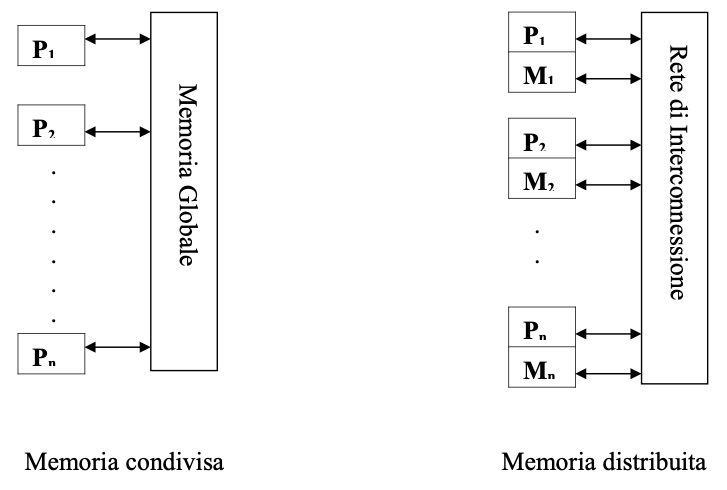
\includegraphics[scale=0.4]{images/memoria_condivisa_distribuita.png}
\end{figure}

Nel modello a memoria condivisa tutti i processori possono accedere alle stesse locazioni di memoria nella stessa unità di tempo. Il meccanismo di comunicazione tra due processori $P_k$ e $P_j$ è molto semplice:
\begin{enumerate}
    \item $P_k$ scrive il messaggio in un’area di memoria
    \item $P_j$ lo legge dalla stessa area
\end{enumerate}
Va segnalato che i processori non sono direttamente connessi e che la comunicazione avviene in tempo costante $O(1)$

Nei modelli a memoria distribuita ogni processore può accedere invece solo alla sua memoria privata (locale). La comunicazione avviene qui attraverso l’invio di messaggi su una rete di interconnessione, che può essere descritta da un grafo i cui vertici sono i processori e i lati rappresentano collegamenti diretti tra processori. \uline{Poiché in tali reti non tutti i processori sono collegati direttamente, non è possibile ipotizzare tempi di comunicazione costanti, contrariamente a quel che succedeva nel caso a memoria condivisa}

Nel parallelo il fattore rilevante è il TEMPO. Valutatiamo il tempo come il numero di clock necessari a far terminare l'algoritmo

\paragraph{Algoritmi distribuiti}
\begin{itemize}
    \item Ognuno ha un proprio clock centrale, con i propri tempi, che non combacia con quello degli altri
    \item Per comunicare tra di loro sono collegati, ma sicuramente possiamo assumere che non hanno una memoria in comune
\end{itemize}

\begin{osservazione}
La comunicazione gioca un ruolo fondamentale e i tempi di sincronizzazione assumono un ruolo principale rispetto ai tempi di esecuzione delle operazioni. La somma di due numeri richiede un semplice clock ma l'attesa di un dato potrebbe richiedere diversi cicli di clock. E' la comunicazione che assume un ruolo più rilevante rispetto al tempo di esecuzione delle operazioni
\end{osservazione}

\uline{Nel distribuito il fattore rilevante è il COORDINAMENTO}.

\paragraph{Esempi di architetture parallele}
\begin{itemize}
    \item Supercomputer: cluster di processori ad elevate prestazioni di calcolo. Questi vengono utilizzati per emulare fenomeni reali, come fenomeni fisici, economici e militari. Simulano sistemi complessi e hanno bisogno di molti processori per il calcolo
    \item GPU: quello che sanno fare molto bene è risolvere operazioni in spazi vettoriali (matrici)
    \item Multicore processor
\end{itemize}

\paragraph{Esempi di architetture distribuite}
\begin{itemize}
    \item Reti di calcolatori connessi a Internet: la rete permette di coprire alte distanze e troveremo i nostri dispositivi di calcolo molto lontani tra di loro. Per questo ci sarà bisogno di un protocollo di comunicazione condiviso che è il \textit{TCP/IP}
    \item Reti mobili: la topologia delle connessioni cambia durante l'esecuzione di un algoritmo. La connessione non è fissata e varia nel tempo
    \item Reti di sensori: piccoli elementi di calcolo che hanno delle capacità limitate e per la maggior parte del tempo stanno in \textit{stand-by} attivandosi con un messaggio di \textit{wake-up} e poi si rimettono in stand-by. Servono per monitorare delle realtà come la temperatura. Hanno bisogno di meccanismi di \textit{wake-up}, \textit{aknowledge}, \textit{recovery}
\end{itemize}

\newpage
\section{Tempo}
\begin{osservazione}
In entrambi i casi, algoritmi paralleli e algoritmi distribuiti, la risorsa tempo è cruciale
\end{osservazione}

\paragraph{Come si misura il tempo?} Il tempo è misurato come la quantità di operazioni elementari richieste per risolvere il problema. 

\paragraph{Tempo nel caso sequenziale} 
$$t(n) = max\;\{T(x)\;|\;x \in \Sigma^n\}$$
In questo caso entra in gioco la definizione formale $T(x)$, è il numero di operazioni elementari che servono per risolvere il problema su un'istanza $x$, dove $x$ è l'input 

Si definisce $t(n)$ il $max$ tra tutti i $T(x)$ dove $x$ è un'istanza di lunghezza $n$. E' la valutazione $T(x)$ nel caso peggiore. E' una funzione in $n$, dove $n$ è la lunghezza dell'input

\begin{osservazione}
    Spesso non saremo interessati ad una valutazione precisa di $t(n)$, ma al suo tasso di crescita, ci basta valutare l'ordine di grandezza, il tasso di crescita della funzione. Per questo useremo le funzioni asintotiche  O,$\;\Omega, \;\Theta$
\end{osservazione}

\begin{figure}[h]
    \centering
    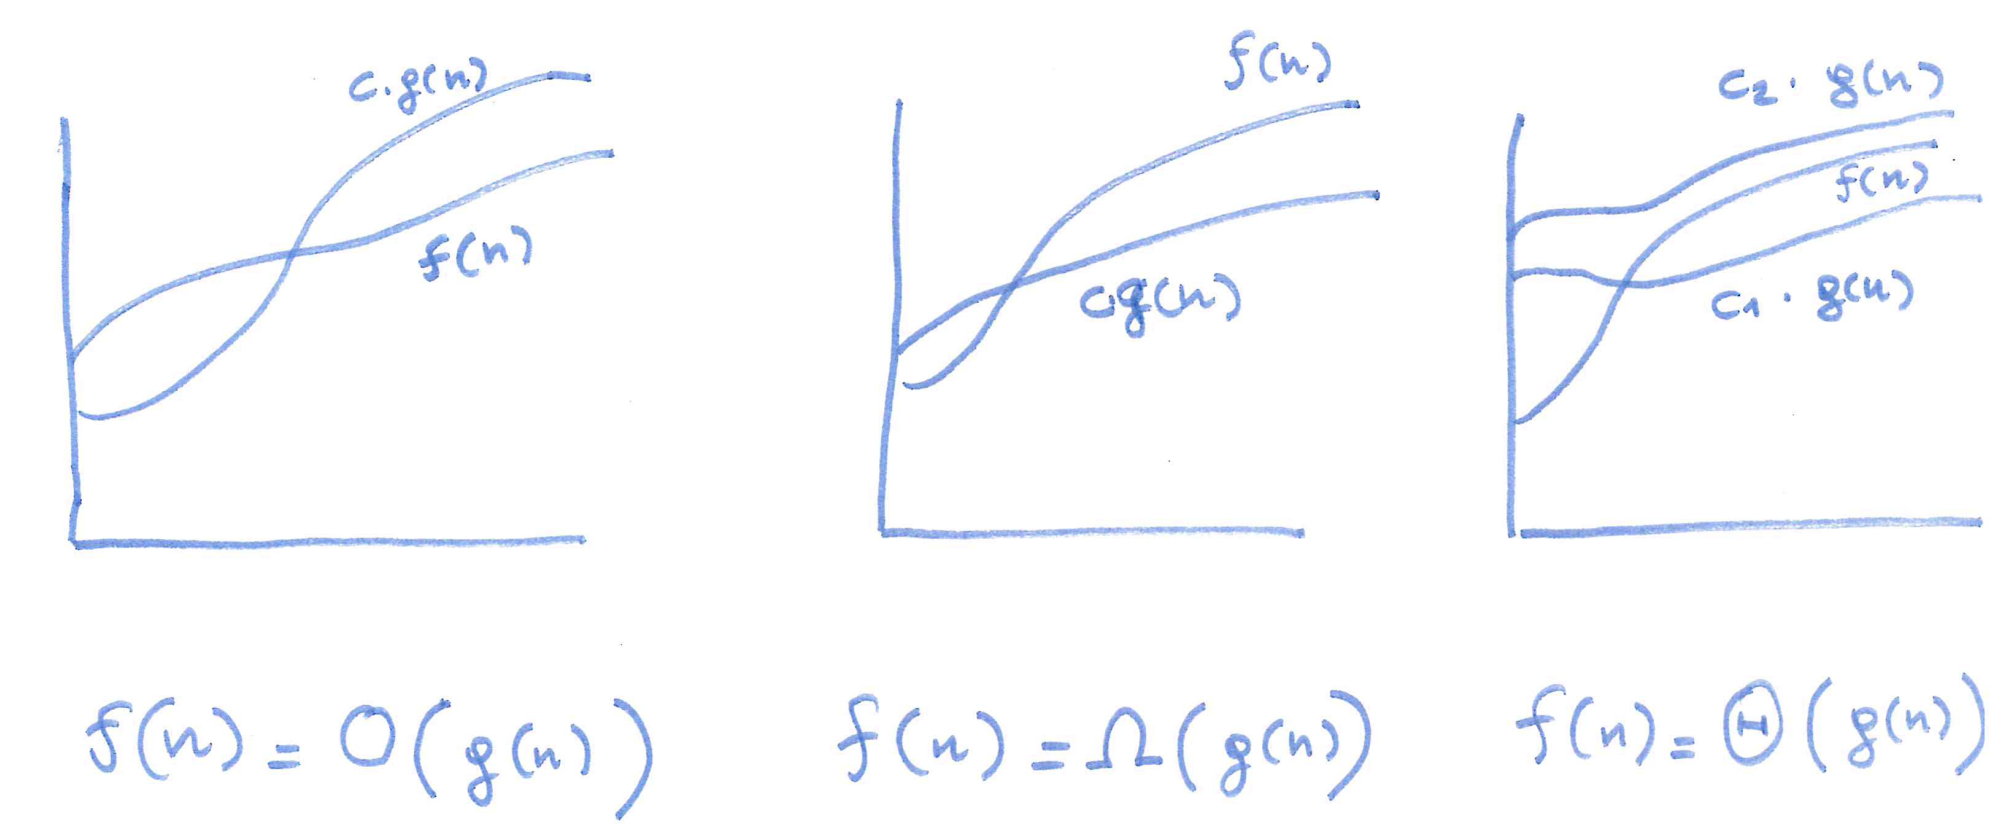
\includegraphics[scale=0.4]{images/funzioni_asintotiche.png}
    \caption{Funzioni asintotiche}
\end{figure}

Quindi O di $log_n$ vuol dire che non cresce più di $log_n$, è limitata superiormente dalla funzione $g(n)$. $\Omega(g(n))$ vuol dire che è limitato inferiormente, quindi può essere più grande di $g(n)$

\paragraph{Avvertenze sulla valutazione di t(n)}
\begin{itemize}
    \item $t(n)$ viene valutata su un particolare modello di calcolo. Quello che contiamo sono le operazioni elementari che il modello di calcolo ci offre
    \item Va scelto il \uline{criterio di costo: \textit{uniforme} o \textit{logaritmico}}. Se utilizzo il criterio di costo uniforme le operazioni elementari richiedono un'unità di tempo, se utilizzo il criterio di costo logaritmico considero le operazioni elementari ma ogni operazione ha un peso che è diverso a seconda della dimensione dei numeri che sono in gioco. Noi useremo il costo uniforme. Il costo logaritmico prende in considerazione anche la dimensione dei dati.
\end{itemize}

\paragraph{Teoria della complessità}
Possibili tassi di crescita di $t(n)$
\begin{itemize}
    \item logaritmico quando è $O(\log n)$
    \item polilogaritmico quando è $O(\log^k n)$ per una costante $k > 0$
    \item lineare quando è $O(n)$
    \item polinomiale quando è $O^k$ per una costante $k > 0$
    \item esponenziale quando NON è $O^k$ per ogni costante $k > 0$
\end{itemize}

\subsection{Concetto di efficienza}
Questa funzione tempo dovrà dirci se i nostri algoritmi sono efficienti.

\paragraph{Caso sequenziale}
Cosa era efficiente nel caso sequenziale? 

Un problema è risolto efficacemente in tempo sse è risolto da una Macchina di Turing deterministica in tempo polinomiale.

Tempo polinomiale $=$ efficienza, perchè? Perchè la classe di problemi risolta in tempo polinomiale (P, FP) risulta essere robusta rispetto a svariati modelli di calcolo. Finchè la funzione tempo è polinomiale i tempi sono ragionevoli, quando diventa esponenziale non vanno bene più.

\paragraph{Classi di problemi}
Quindi \textit{P} ed \textit{FP} hanno una definizione robusta che non cambia con il modello di calcolo. Purtroppo altri problemi interessanti non hanno ancora soluzioni efficienti e stanno in \textit{NP}: problemi di decisione risolti in tempo polinomiale su una Macchina di Turing non deterministica. Esempio la fattorizzazione di interi, utile per algoritmi di crittografia. 

I problemi in \textit{NP} sono quei problemi di cui non si sa se esiste un algoritmo polinomiale per essi.

L'efficienza nel caso parallelo è \textit{NC}. Ciò che si sa è che $NC \in FP$. Cioè se ho un algoritmo parallelo efficiente per un certo problema ho anche un algoritmo sequenziale efficiente e la cosa è vera perchè prendo l'algoritmo parallelo lo do ad un processore che esegue in sequenza le istruzioni del mio algoritmo parallelo. Siccome risulta essere efficiente nel caso parallelo, risulta essere efficiente anche nel caso sequenziale. Sono quei problemi risolti con algoritmi paralleli veloci, cioè tempo poli-logaritmico, ad esempio $log_4(n)$ o $log_3(n)$ e hardware polinomiale, anche l'hardware ha un limite superiore. Non possiamo dire che un problema viene risolto in modo efficiente nel mondo parallelo se utilizziamo ad esempio un hardware esponenziale, perchè risulta impraticabile per istanze anche molto piccole dell'input. I problemi che stanno in NC sono quelli altamente parallelizzabili che stanno in FP

$NC = FP$? Problema aperto, si pensa di no! Rispondere a questa domanda è come rispondere alla domanda: ogni algoritmo efficiente è parallelizabile (rimanendo chiaramente efficiente)?

Le classi di problemi P, FP, NP e NC sono classificazioni utilizzate per descrivere la complessità temporale degli algoritmi utilizzati per risolvere i problemi
\begin{itemize}
    \item La classe P (Polynomial) include tutti i problemi per i quali esiste un algoritmo di soluzione efficiente, ovvero che ha una complessità temporale polinomiale
    \item La classe FP (Functional Polynomial) include tutti i problemi per i quali esiste un algoritmo di verifica efficiente, ovvero che ha una complessità temporale polinomiale, ma per i quali non esiste un algoritmo di soluzione efficiente
    \item Per la classe NP non esiste un algoritmo di soluzione efficiente per questi problemi, ovvero con complessità temporale polinomiale  
    \item La classe NC (Non-deterministic Polylogarithmic) include tutti i problemi per i quali esiste un algoritmo di soluzione con complessità temporale poli-logaritmica
\end{itemize}



\newpage
\section{Caso parallelo PRAM - Parallel RAM}
Consiste di un set di processori che hanno una memoria in comune. Questa memoria condivisa fa si che la comunicazione tra i processori sia immediata.

C'è una memoria centrale su cui si affacciano i processori. Questi processori avranno anche la memoria privata perchè per lavorare hanno bisogno anche di registri personali.

La memoria globale è usata dai processori per scambiarsi dati in tempo $O(1)$: perché il processore $k$ e il processore $j$ si scambino un valore, basta che il processore $k$ scriva tale valore in una variabile condivisa e il processore $j$ vi acceda in lettura. Il calcolo procede per passi.

Questo modello di macchine è detto di tipo SIMD (Single Instruction Multiple Data).

\paragraph{Risorse di calcolo} Sono il tempo parallelo richiesto dal nostro algoritmo e il numero di processori, cioè la quantità di hardware messa a disposizione per risolvere il problema
\begin{itemize}
    \item sequenziale: $t(n), s(n)$
    \item parallelo: $p(n), T(n,p(n))$. Dove $n$ è la lunghezza dell'input, $p(n)$ il numero di processori su input di lunghezza $n$ (caso peggiore). E' ovvio che il tempo dipenda non solo dalla lunghezza dell'input ma anche dal numero di processori presi in considerazione.

    $T(n)$ era vero anche nel caso sequenziale, in questo caso diventa anche funzione di $p(n)$, perciò $T(n, p(n))$. Il tempo parallelo dipende anche dal numero di processori utilizzati per l'esecuzione dell'algoritmo

    Quando leggeremo $T(n,1)$ è un caso particolare del tempo parallelo che coincide con il tempo sequenziale. Come caso particolare degli algoritmi paralleli ci sono gli algoritmi sequenziali
\end{itemize}

\paragraph{Valutazione precisa del tempo T(n, p(n))}
Mettiamo la nostra batteria di processori in fila $P_1, P_2, \dots, P(n)$ e metto in colonna le istruzioni eseguite dal processore. \uline{Ogni riga di questa tabella mi dà un passo parallelo}. \uline{Il numero di passi paralleli solitamente dipende dal numero di $n$, l'ultimo passo è $k(n)$}.

\uline{Per ogni passo parallelo prendo il tempo massimo e sommo}. Così ottengo il tempo totale dell'algoritmo. Il tempo del passo i-esimo lo indichiamo così
$$t_i(n) = max\{t_i^j(n)\;|\;1 \leq j \leq p(n)\}$$
E' il massimo tra tutti i tempi dell'i-esimo passo tra tutti i processori $j$.\\
Pertanto il tempo massimo di questo algoritmo non è altro che la somma del tempo richiesto all'i-esimo passo per i che va da 1 a $k(n)$
$$T(n,\;p(n)) = \sum_{i=1}^{k(n)}\;t_i(n)$$
\begin{itemize}
    \item $T$ dipende da $k(n)$
    \item $T$ dipende anche dalla dimensione dell'input $n$
    \item $T$ dipende da $p(n)$
\end{itemize}

Se al posto di $p(n)$ processori ne abbiamo $p(n/2)$, quindi li riduciamo, allora $p1$ esegue le sue istruzioni del primo passo parallelo più le istruzioni che seguono del processore $p(n/2) + 1$. $p2$ eseguirà le sue istruzioni del primo passo parallelo e successivamente le istruzioni di $p(n/2) + 2$ e così via.

\paragraph{Proprietà sulla comunicazione} La comunicazione avviene in tempo costante, infatti se un processore $P_j$ vuole comunicare un dato $x$ a $P_z$ prende dal suo registro personale il dato $x$ e lo scrive in un registro della memoria centrale. $P_z$ sa che è avvenuta questa operazione e va a leggere il dato nella memoria centrale. Questa è la situazione dei multi-core attuali

Con questa struttura siamo in grado di attuare una \uline{forte parallelizzazione, il motivo è dato proprio dalla comunicazione in tempo costante}. Non abbiamo problemi a far comunicare processori anche di indici molto distanti. Non si spreca tempo per la comunicazione, il tempo viene utilizzato tutto per far funzionare i processori sulle istruzioni dell'algoritmo.

\paragraph{Memoria condivisa} La memoria condivisa la chiamiamo \textit{M}, questa memoria condivisa è fatta da una sequenza di registri (per semplicità) che chiamiamo $M[0], M[1], \dots, M[n]$.

Ogni $P_i$ è una RAM sequenziale costituita da una ALU e i suoi registri personali che costituiscono la memoria privata del processore li indicheremo con $R[0], R[1]$. 

\begin{osservazione}
  Quando un'unità di calcolo deve compiere un'operazione (ad esempio una somma) deve avere i dati nella sua memoria privata su particolari registri, dove vengono presi le sequenze di bit e sommati. Anche se parleremo di somma di elementi presi dalla memoria centrale c'è questo passaggio di prendere i dati dai registri $M$ e portarli nei registri privati $R$. Siccome però questa operazione è costante\footnote{Perchè facciamo riferimento al costo uniforme, non logaritmico}, e sempre uguale qualunque sia il dato, faremo somme di numeri in $M$ ma in realtà i dati vengono trasportati da $M$ a $R$  
\end{osservazione}

\paragraph{Istruzioni dei Pi}
Ogni singolo processore nella PRAM, essendo a sua volta una RAM, può effettuare le seguenti operazioni:
\begin{itemize}
    \item Operazioni aritmetico/logiche
    \item Istruzioni da/per la memoria centrale:
    \begin{itemize}
        \item $STORE\;R[K]\;M[h]$, prendi il dato dalla mia memoria privata che sta nel mio registro k-esimo e mettilo nella memoria centrale
        \item $LOAD\;R[K\prime]\;M[h\prime]$, operazione opposta. Prendi il dato che c'è nella memoria centrale nella cella $h\prime$ e portalo nella memoria privata.
    \end{itemize}
\end{itemize}

%Come si programma una PRAM
\begin{comment}
 \paragraph{Come si programma una PRAM?}
L'idea è che c'è un unico programma per tutti i nostri processori, tutti hanno accesso al programma e si caricano le istruzioni una dopo l'altra.   
\end{comment}

\paragraph{Architetture in base alla capacità di accedere alla memoria condivisa}
\begin{enumerate}
    \item \textbf{\textit{EREW}}: no scrittura/lettura stessa cella di $M$. \uline{Non è possibile l'accesso simultaneo alle celle della memoria centrale}. Ad un instante di tempo una cella di memoria può essere letta o scritta da soltanto un processore.
    \item \textbf{\textit{CREW}}: lettura simultanea si, scrittura simultanea no. La scrittura rimane esclusiva
    \item \textbf{\textit{CRCW}}: scrittura/lettura simultanea si. Per la scrittura simultanea abbiamo diverse politiche:
    \begin{itemize}
        \item common, i processori possono scrivere in memoria centrale contemporaneamente solo se vogliono scrivere lo stesso dato pena l'arresto del sistema. Se un processore non è sincronizzato, ha un dato diverso e io faccio l'arresto del sistema.
        \item random, un processore a caso scrive. E' una politica difficile
        \item max/min, si permette al processore $P_i$ solo se ha il dato max o min
        \item priority, scrive il processore $P_i$ con priorità max. I processori non sono tutti uguali ma c'è un certo ordine di importanza. 
    \end{itemize} 
\end{enumerate}

\begin{osservazione}
$\text{EREW} \implies \text{CREW} \implies \text{CRCW}$\\
Non è vero il viceversa, perchè architettura di tipo $2$ e $3$ offrono dei vantaggi rispetto all'architettura di tipo $1$. La \textit{CREW} ha la scrittura simultanea e questo velocizza il nostro algoritmo. L'architettura più ragionevole e semplice a livello hardware è EREW, in questo caso è compito del programmatore disegnare l’algoritmo in modo che non accadano conflitti in lettura o scrittura
\end{osservazione} 

\paragraph{Forma dell'istruzione}
Chiamato anche passo parallelo:
$$for\;all\; i \in I\;par\;do: istruzione_i$$
\textit{par do} cioè fai in parallelo, esegui in parallelo. Si differenzia dal for tradizionale proprio da questo costrutto.

Che cos'è $istruzione_i$?A seconda delle architetture della nostra PRAM abbiamo diverse interpretazioni. Ci sono architetture hardware diverse:
\begin{itemize}
    \item \textit{SIMD}: single instruction multiple data.\\
    L'istruzione è uguale per tutti i processori però avviene su dati diversi, su diversi registri.
    \item \textit{MIMD}: multiple instruction multiple data\\
    Abbiamo la possibilità per processori diversi di eseguire istruzioni differenti
\end{itemize}

%Sintesi

\paragraph{Valutazione}
Cos'è efficiente nel caso parallelo? Nel caso sequenziale è \textit{P}, problemi risolti in tempo polinomiale, nel caso parallelo deve essere meglio del tempo polinomiale.

Definiremo un parametro \textbf{\textit{E}: efficienza}, che tiene conto sia del tempo impiegato dal nostro algoritmo che del numero di processori. Se devo avere un'esplosione esponenziale dei processori non conviene. Quindi il tempo deve essere migliore e i processori devono essere contenuti, altrimenti non conviene. Il parametro efficienza ci deve dire se la nostra soluzione parallela è preferibile ad una efficiente soluzione sequenziale

Valuteremo la nostra funzione di tempo $T(n, p(n))$ con il tempo richiesto dall'algoritmo sequenziale $T(n, 1)$. \uline{Se la nostra funzione ha un tasso di crescita inferiore rispetto a quella sequenziale vuol dire che abbiamo migliorato la nostra soluzione}. 
Abbiamo due casi
\begin{itemize}
    \item $T(n,p(n)) = \Theta (T(n,1))$, uguale al tempo sequenziale. Vuol dire che è limitato superiormente e inferiormente dalla funzione sequenziale $T(n,1)$. Il tasso di crescita del tempo parallelo è circa uguale, asintotica alla funzione $T(n,1)$ di tipo sequenziale. E' il caso che noi vogliamo evitare
    \item $T(n,p(n)) = o(T(n,1))$. Vuol dire che cresce più lentamente rispetto al tempo sequenziale. Se faccio il rapporto tra tempo sequenziale e tempo parallelo ho qualcosa che tende ad infinito. E' il caso che vogliamo
\end{itemize}

\paragraph{Speed-up} 
$$S(n, p(n)) = \frac{T(n, 1)}{T(n, p(n))}$$
Esempio: $S=4$ l'algoritmo parallelo è $4$ volte più veloce del sequenziale, ma ricadremo nel primo caso. Quello che vogliamo è che lo \textit{speed-up} sia infinito perchè così abbiamo il secondo caso.
$$S(n,p(n)) \rightarrow \infty$$
Questo non ci dice niente rispetto al valore della risorsa $p(n)$, magari abbiamo utilizzato un numero di processori esagerato. \uline{Non riusciamo a considerare il numero dei processori}. Questo parametro perciò viene utilizzato solo per definire successivamente il parametro efficienza.

\paragraph{Efficienza}
$$E(n,p(n)) = \frac{S(n,p(n))}{p(n)} = \frac{T(n,1)*}{p(n)T(n,p(n))}$$
* si intende il tempo del miglior algoritmo sequenziale. Andiamo a scegliere la funzione tempo più piccola possibile.

Se $E \rightarrow 0$ non va bene, infatti dato che $T(n,p(n)) = o(T,(n,1))$ deve essere che $p(n)$ cresce troppo velocemente. 

Perchè se tende a $0$ stiamo usando troppi processori? Quando lo \textit{speed-up} tende ad infinito vuol dire che i tempi vanno bene, cioè il parallelo è un o piccolo del sequenziale. Se il tempo parallelo non abbatte il tempo sequenziale devono essere i processori che abbattono il tempo sequenziale e quindi stiamo utilizzando troppi processori.

$$0 \leq E(n, p(n)) \leq 1$$

Che sia positivo si vede dalla formula. Che invece il parametro \textit{E} non supera il valore $1$ è da dimostrare.

%Se E->0 stiamo usando troppo hw
\begin{comment}
Esempio: soddisficibilità di formule
$$E(n,p(n)) = \frac{2^n}{2^n\;n} = \frac{1}{n} \rightarrow 0$$
Quando $E \rightarrow 0$ il nostro algoritmo non è così buono perchè ha un costo hardware toppo alto. Stiamo utilizzando troppi processori.
\end{comment}

\begin{dimostrazione}
\textbf{Attraverso algoritmo parallelo $\rightarrow$ algoritmo sequenziale}

Come possiamo ottenere un algoritmo sequenziale se noi abbiamo un algoritmo parallelo? Sostituiamo a $p(n)$ processori un processore solo e mandiamo in esecuzione tutte le istruzioni del primo passo, poi del secondo, etc. Ora vogliamo valutare il tempo di esecuzione dell'algoritmo sequenziale che otteniamo. 

Chiamo $\Tilde{T}(n,1)$ il tempo richiesto dall'algoritmo sequenziale che ho appena descritto, ottenuto direttamente dall'algoritmo parallelo.
Otteniamo un particolare algoritmo sequenziale e il tempo è sicuramente peggiore del miglior algoritmo sequenziale $T(n,1) \leq \Tilde{T}(n,1)$

Il tempo massimo del primo passo parallelo è $t_1(n)\;\text{,}\;p(n) * t_1(n)$ perchè devo fare $p(n)$ mini-programmi, perciò
$$T(n,1) \leq \Tilde{T(n,1)} \leq pn\;t_1(n) + pn\;t_2(n) \dots p(n)\;t_{k(n)}(n)$$

Ora posso raccogliere a fattor comune $p(n)$ e ottengo $p(n)\;\sum_{i=1}^{k(n)}\;t_i(n)$ dove $t_i(n)$ è il tempo di ogni singolo passo parallelo. Ma quest'ultima parte non è nient altro che il tempo parallelo $p(n)T(n,p(n))$

Quindi abbiamo che il miglior tempo sequenziale $T(n,1)$ è limitato superiormente da $p(n)T(n,p(n))$ cioè $p(n)$ per il tempo parallelo. Si ottiene 
$$T(n,1) \leq p(n)\;T(n,p(n))$$
Cosa succede se dividiamo entrambo i lati di questa disuguaglianza per $p(n)$?

$$\frac{T(n,1)}{p(n)} \leq T(n,p(n))$$

Otteniamo che \uline{il nostro tempo parallelo ha un lower bound}, ha un limite inferiore, e questo limite è dato dal rapporto tra il miglior tempo sequenziale diviso il numero di processori. Cioè la cosa migliore che io posso fare è prendere il miglior algoritmo sequenziale ed equi-distribuire le istruzioni tra tutti i processori che lavorano per parallelizzare l'algoritmo.

Ora dividiamo anche per il tempo parallelo $T(n,p(n))$, significa portarlo a sinistra della disuguaglianza, otteniamo a sinistra il parametro efficienza e a destra otteniamo $1$

$$\frac{T(n,1)}{p(n)T(n,p(n))} \leq 1 \equiv E(n,p(n)) = 1$$

Abbiamo dimostrato che l'efficienza non può essere più grande di $1$.
Il meglio che posso avere è $E \rightarrow K \leq 1$ dove $K$ è una costante limitata da $1$ superiormente
\end{dimostrazione}

\begin{dimostrazione} Principio di Wyllie

    \textit{"Se $E \rightarrow 0$ allora per migliorare l'algoritmo provo a ridurre $p(n)$ senza degradare il tempo"}

    Studiare il parametro efficienza facendo crescere/diminuire il numero di processori, cambiando il numero di processori nella formula.

    In particolare è stata data la ricetta di J.Wyllie nella sua tesi del PhD che dice la seguente cosa:
    Se noi diamo un algoritmo parallelo, calcoliamo il parametro efficienza e questo tende a $0$ allora non necessariamente va buttato l'intero algoritmo ma forse si può fare qualcosa per migliorare il parametro efficienza e quindi ottenere un algoritmo buono. Si può migliorare provando a ridurre il numero di processori senza però degradare troppo il tempo (non devo avere un tempo che cambia il tasso di crescita).

    Vediamo la validità di questo principio cambiando il numero di processori da $p\; \text{a}\; \frac{p}{k}$. Raggruppo $p$ lavori a $k$, quindi \uline{un processore anzichè trovarsi $1$ programma se ne trova $k$ e li deve eseguire in sequenza}. Quanto tempo richiede per eseguire $k$ lavori? Il tempo di ogni programmino è limitato superiormente da $k\;t_i(n)$ perchè $t_i(n)$ è il massimo tempo richiesto tra tutti i programmini all'i-esimo passo e non può essere superiore a $k\;t_i(n)$ perchè ne esegue $k$ che vengono eseguiti in sequenza.

    Il tempo parallelo richiesto dal nostro algoritmo fatto in questo modo è limitato superiormente dalla somma dell'i-esimo passo parallelo. Ma l'i-esimo passo parallelo è limitato da $kt_i(n)$. Otteniamo
    $$T(n, \frac{p}{k}) \leq \sum_{i=1}^{k(n)} k\;t_i(n) = k T(n,p)$$

    Questo $k$ è in comune ad ogni elemento della sommatoria perciò posso raccogliere $k$ fuori dalla sommatoria e ottengo

    $$T(n,\frac{p}{k}) \leq k\;T(n, p)$$
    
    Il tempo dell'algoritmo che utilizza $\frac{p}{k}$ processori anzichè $p$ processori è limitato superiormente da $k$ volte il tempo richiesto dall'algoritmo che utilizza $p$ processori.

    Partendo da questa disuguaglianza quello che si ottiene è che \uline{il parametro E cresce col diminuire dei processori}. Questo è vero tenendo la funzione tempo parallelo fissata, cioè senza far degradare troppo il tempo. Quanto vale $E(n, \frac{p}{k})$?
    $$E(n,\frac{p}{k}) = \frac{T(n,1)}{\frac{p}{k}\;T(n,\frac{p}{k})} \geq \frac{T(n,1)}{\frac{p}{k}\;kT(n,p)} = E(n,p)$$

    La formula mostra che diminuendo i processori migliora il parametro efficienza (ciò rende vera la ricetta di Wyllie). \uline{In sostanza ottengo il rapporto tra tempo sequenziale e tempo parallelo su $p$ processori (dopo le semplificazioni), questo per definizione non è nient'altro che l'efficienza su $p$ processori}. \uline{Quindi diminuendo il numero di processori da $p$ a $\frac{p}{k}$ l'efficienza migliora}.

    Vediamo se $k$, nella formula di prima, lo facciamo tendere a $p$ in modo da voler verificare cosa succede se diminuisco il numero di processori aumentando $k$. Sempre meno processori arrivando all'estremo fino ad arrivare ad avere $\frac{p}{p}$

    $$1=E(n,1)=E(n,\frac{p}{p}) \geq E(n,\frac{p}{k}) \geq E(n,p)$$

    (A destra) se confronto l'algoritmo con $\frac{p}{k}$ e quello con $p$ il primo mi da un efficienza migliore. (A sinistra) ho diminuito i processori ($\frac{p}{p}$) e quindi l'efficienza migliora, ecco perchè ho un $\geq$. Però questa non è altro che l'efficienza calcolata con un processore $E(n,1)$ che è sostanzialmente il tempo sequenziale (perchè avrò tempo sequenziale su tempo sequenziale, cioè $1$).

    In questo modo abbiamo ottenuto che l'efficienza di un algoritmo parallelo che usa $p$ processori è limitata superiormente da $1$.
\end{dimostrazione}

\newpage


\subsection{Sommatoria}
Utilizziamo più processori, ogni processore si prende una somma e poi una volta ottenuti gli esiti parziali dobbiamo fonderli per ottenere il risultato della sommatoria

Input: $M[1], M[2], \dots , M[n]$\\
Output: $M[n] = \sum_{i=1}^n M[i]$

Supponiamo che i valori $n$ siano nella memoria centrale, quindi nelle celle $M[1], M[2], \dots , M[n]$. Il risultato lo scriveremo nell'ultima cella $M[n]$.

\paragraph{Algoritmo sequenziale}
Il migliore algoritmo sequenziale è dato da questo codice
\begin{lstlisting}
    for i=1 to n-1 do
        M[n] = M[n] + M[i]
\end{lstlisting}
Siccome vogliamo il risultato in $M[n]$ questo algoritmo somma tutto in $M[n]$ utilizzandolo come un accumulatore, escludendo chiaramente $n$ perchè viene sommato alla prima iterazione. Quante istruzioni sono? $n-1$ per cui il tempo di questo algoritmo sequenziale è proprio $T(n,1) = n-1$ e non posso scendere al di sotto di questo valore perchè le somme devo farle tutte.

\paragraph{Idea per parallelizzare} "Una somma a processore", ma in questo modo non stiamo dicendo quale somma

\begin{figure}[h]
    \centering
    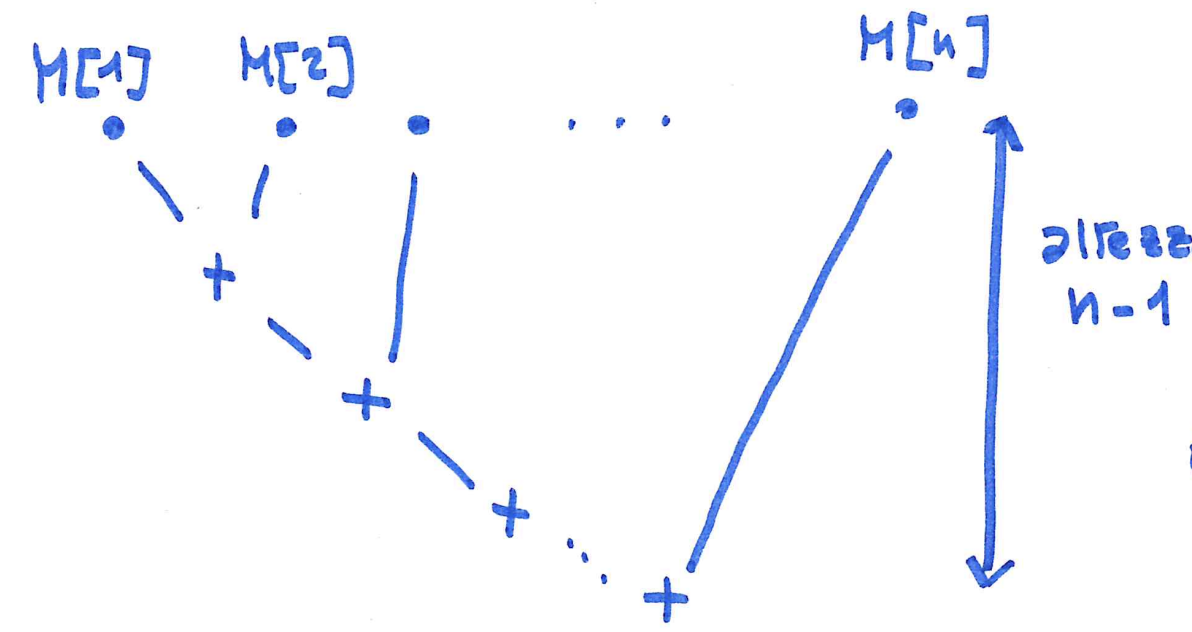
\includegraphics[scale=0.4]{images/idea_sommatoria.png}
\end{figure}

Rappresentiamo il nostro algoritmo come un albero (sbilanciato) che ha come foglie i dati di input, le celle $M[1], M[2], M[n]$, e i livelli dell'albero rappresentano i passi paralleli del nostro algoritmo. Ogni livello di quest'albero è un passo parallelo e mi vengono fuori $n-1$ passi. Qual'è l'efficienza di questo algoritmo?

$$E=\frac{n-1}{(n-1)(n-1)} \rightarrow 0$$

Il tempo sequenziale sopra che abbiamo calcolato dall'algoritmo sequenziale. Ogni processore fa una somma perciò avrò $n-1$ somme quindi $n-1$ processori per il tempo dell'algoritmo parallelo che è $n-1$. Tende a $0$ quindi non è efficiente. Se il tempo è uguale al sequenziale non ho parallelizzato niente, non ha senso calcolare il parametro efficienza. \uline{L'altezza risulta essere il tempo dell'algoritmo}.

\paragraph{Alternativa} Posso fare qualcosa di diverso perchè la somma è associativa\footnote{$((a+b)+c)+d = (a+b) + (c+d)$}, non conta l'ordine con cui facciamo le somme. In più da un albero \textit{sbilanciato} mi muovo su un albero \textit{bilanciato}

\begin{figure}[h]
    \centering
    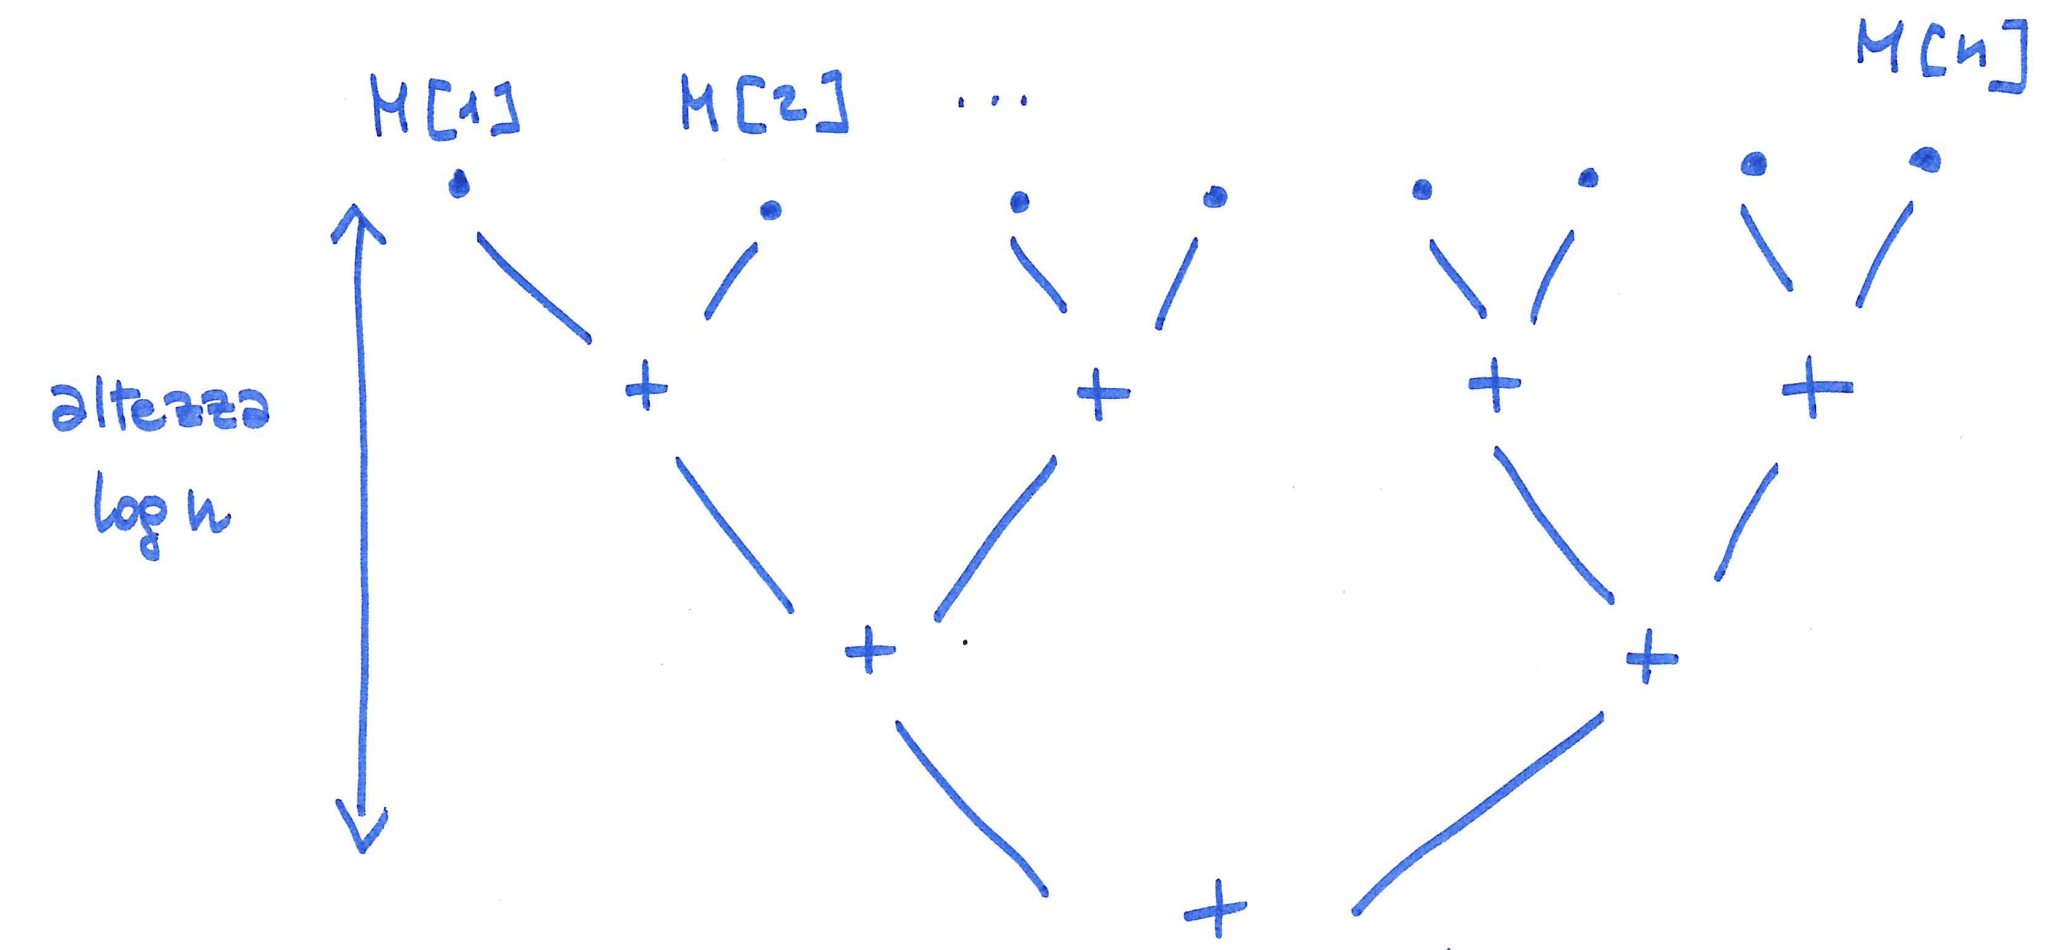
\includegraphics[scale=0.35]{images/idea2_sommatoria.png}
    \caption{Alternativa per parallelizzare}
\end{figure}

\uline{Stiamo assumendo che $n$ è potenza di $2$}. Cosa manca in questo schema? Non abbiamo detto come fanno i processori a comunicarsi gli esiti. L'idea è che li vanno a \uline{sovra-scrivere nelle celle di memoria dell'input}.

\paragraph{Algoritmo EREW}
In questo caso le celle sono lette e scritte in maniera esclusiva, non ci sono letture e scritture simultanee. In una PRAM serve sapere anche dove andiamo a memorizzare gli esiti parziali perchè tutti i processori devono essere d'accordo sulla cella condivisa che contiene il risultato.

\begin{figure}[h]
    \centering
    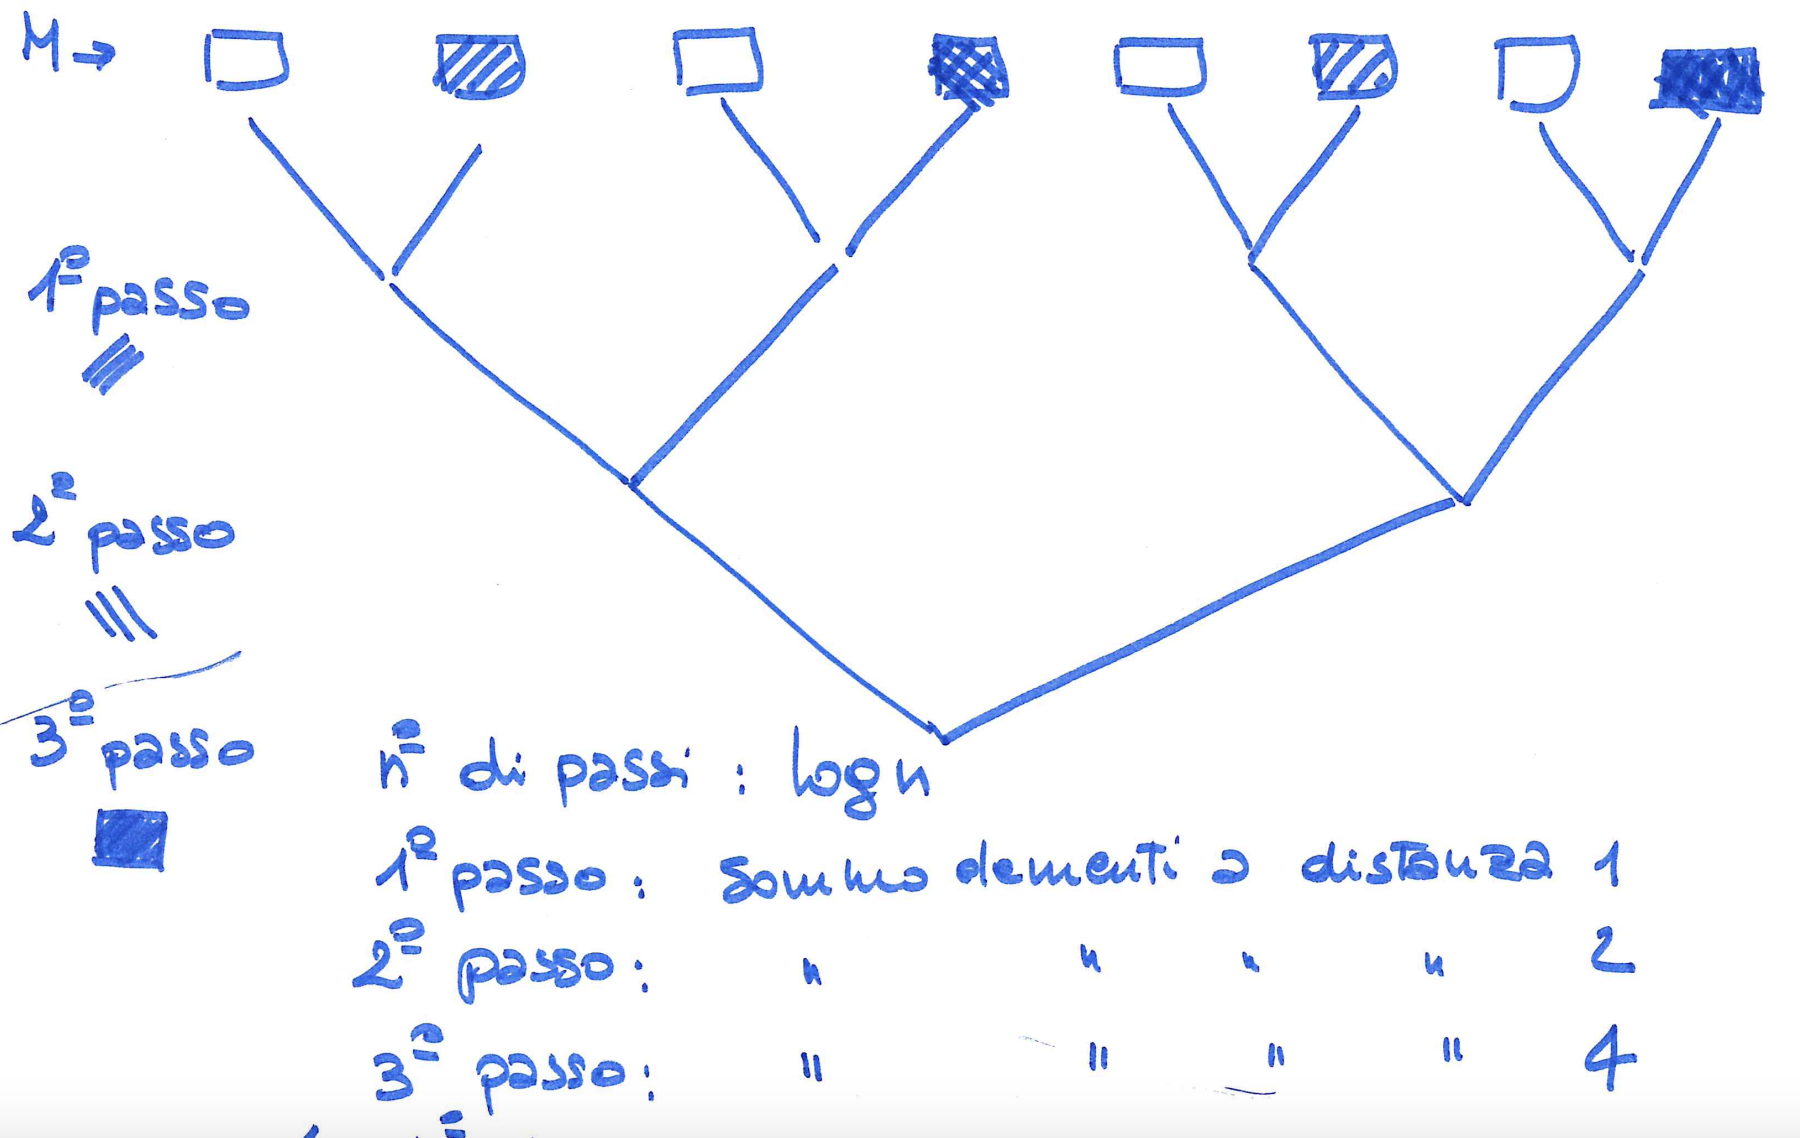
\includegraphics[scale=0.4]{images/erew_sommatoria.png}
    \caption{Algoritmo EREW sommatoria}
\end{figure}

\uline{Il risultato si pone nella cella con indice più alto}. Al primo passo si somma l'indice dispari con quello pari. Al secondo passo i processori sanno che i dati su cui calcolare la somma sono quelli di indice pari. La distanza è una potenza di $2$ e aumenta man mano che aumenta l'indice del passo parallelo. Il numero di passi di questo algoritmo risulta essere $\log n$ perchè abbiamo un albero completamente bilanciato

Istruzioni:
Consideriamo \textit{k} come gli indici dei processori e i passi sono paralleli
\begin{enumerate}
    \item passo: $M[2k] = M[2k] + M[2k-1]$ con $1 \leq k \leq \frac{n}{2}$
    \item passo: $M[4k] = M[4k] + M[4k-2]$ con $1 \leq k \leq \frac{n}{4}$
    \item passo: $M[8k] = M[8k] + M[8k-4]$ con $1 \leq k \leq \frac{n}{8}$
    \item $\dots$
    \item $\log n$ passo: $M[n] = M[n] + M[\frac{n}{2}]$ 
\end{enumerate}

\paragraph{Pseudo-codice} Dove $j$ è l'indice del passo parallelo
\begin{minted}
    [
    frame=lines,
    framesep=2mm,
    baselinestretch=1.2,
    bgcolor=white,
    fontsize=\footnotesize,
    linenos
    ]{python}
    for j in range(1, logn):
        for k in range(1, n // 2**j + 1):
            M[2**j*k] = M[2**j*k] + M[2**j*k - 2**(j-1)]
    return M[n]
\end{minted}
Il primo ciclo for scandisce i passi paralleli (l'indice dei passi paralleli è j), il secondo è un for par do quindi è un passo parallelo e fa lavorare $\frac{n}{2^j}$ processori al passo $j$ 

\paragraph{Dimostrazione EREW}
E' \textit{EREW}? Solo il processore \textit{k} può leggere e fare operazioni, gli altri utilizzano altre celle.

Come due processori $a$ e $b$ che lavorano nello stesso passo parallelo le celle che vanno a toccare risultano essere diverse tra di loro.

\begin{dimostrazione}
Dobbiamo dimostrare che al j-esimo passo vale questa proprietà
$$M[2^jk]=M[2^jk]+ \dots + M[2^j(k-1)+1]$$
Dove $j$ è un qualcosa compreso tra $[1, \log n]$, l'indice del passo parallelo. Dobbiamo dimostrare che nelle celle multiple di $2^j$ ci sono $2^j$ valori sommati di tutte le $2^j$ celle precedenti  

La dimostrazione è una dimostrazione per induzione su j. Andiamo a sostituire nella star (prima equazione) $\log n$ al posto di $j$. Inoltre siccome siamo al passo $\log n$ sappiamo che viene utilizzato un solo processore che è quello che fa la somma dei due risultati parziali che lavorano sulla metà dell'input. Allora $k=1$ perchè c'è un solo processore. In questo caso la proprietà è
$$M[n] = M[n] + \dots + M[1]$$
Mi viene che in $M[n]$ ci va la somma di tutti i precedenti valori. Se è vera questa proprietà, questo dimostra che il mio algoritmo è corretto.

CASO BASE: $j=1$ e $1 \leq k \leq \frac{n}{2}$\\
Istruzione dell'algoritmo $\rightarrow M[2K] = M[2K] + M[2K-1]$ quindi vale la proprietà star 

PASSO INDUTTIVO: Supponiamo vera la proprietà star per l'indice $j-1$ e dimostriamo che la manteniamo anche per il passo successivo, dimostriamo che vale anche per $j$
\end{dimostrazione}

\subsubsection{Valutazione dell'algoritmo sommatoria}

\paragraph{Numero di processori}
Il numero di processori $p(n) = \frac{n}{2}$. Il livello più costoso in termini di processori è il primo, quindi prendo quello. E' vero che al passo successivo la metà di questi sono inutilizzati, ciò potrebbe suggerirci che stiamo usando troppi processori

\paragraph{Tempo}
Abbiamo detto che l'altezza dell'albero è $\log n$ perciò il tempo deve essere logaritmico, andiamo a considerare le micro-istruzioni: LD, LD, ADD, ST. $4$ micro-istruzioni, perciò il tempo parallelo calcolato su $T(n, \frac{n}{2}) = 4 \log n$

\begin{osservazione}
    Un piccolo accorgimento dobbiamo farlo se $n$ non è potenza di $2$. Abbiamo detto che lavora bene su $n$ potenza di $2$ perchè ci da un albero bilanciato. Idea: allunghiamo l'input di $0$ fino alla potenza di $2$ successiva ad \textit{n}. Cioè da \textit{n} binario a $2n$. Va bene mettere lo $0$ perchè non modifica il risultato totale. 

    La potenza più vicina ad \textit{n} la posso trovare in binario. Cioè da \textit{n} in binario la successiva potenza di due ha un bit in più impostato ad $1$ e poi $0$, cioè $1 0 0 \dots 0$. Questa distanza di $2$ la troviamo tra \textit{n} e $2n$, infatti se scriviamo $2n$ in binario è \textit{n} in binario a cui abbiamo aggiunto uno $0$ finale.

    Pertanto avrò:\\
    $p(n) = \frac{2n}{2} = n$ ; 
    $T(n,n) = 4 \log 2n \leq 5 \log n$ ;\\
    $\implies p(n) = O(n)$ e $T(n,n) = O(\log n)$

    Se non vogliamo considerare le costanti possiamo dire che abbiamo un algoritmo parallelo il quale ha numero di processori lineare $O(n)$ e tempo parallelo $O(\log n)$

    \paragraph{Efficienza}
    $E(n,n) = \frac{n-1}{n\;5\log n} \approx \frac{N}{5 \log n} \rightarrow 0$ lentamente
    
    Sopra il tempo sequenziale. Sotto abbiamo il numero di processori che è $n$ per $\log n$ che è il tempo parallelo, si  semplifica $n$ rimane $\frac{1}{\log n}$ che tende a $0$, lentamente ma tende a $0$
\end{osservazione}

\paragraph{Principio di Wyllie}
Visto che i processori sono un pò sprecati applicchiamo Wyllie, vediamo se riusciamo a diminuire il numero di processori e cerchiamo di mantenere lo stesso tempo per avere $p(n) = o(n) \wedge E \rightarrow C \neq 0$

Invece di avere $\frac{n}{2}$ ci sono solo p processori e andiamo a vedere che valore ci va bene. Questi processori non dovranno prendersi solo due valori in carico ma un po di più perchè $p < \frac{n}{2}$. Supponiamo che il numero di dati che si prende in carico ogni singolo processore sia un valore $\Delta$, cioè sto raggruppando n numeri in p gruppi. $\Delta = \frac{n}{p}$

Abbiamo scoperto che un \textit{p} ragionevole c'è ed è $\frac{n}{\log n}$, allora con un numero di processori $p = \frac{n}{\log n}$ otteniamo un'efficienza costante $\neq 0$. Quindi se noi raggruppiamo i nostri $n$ lavori in gruppi di cardinalità $\log n$ raggiungiamo il nostro scopo. Il numero di processori che prima era $n$ diventa $\frac{n}{\log n}$ e il tempo rimane comunque parallelo perchè il primo passo che consiste nella sequenzializzazione dei $\log n$ lavori che sono stati raggruppati e affidati ai $p$ processori consiste di un tempo che è $\log n$.

 Il primo passo parallelo che è la sequenzializzazione di $\log n$ somme, costa $\log n$. E' un passo parallelo ma questi numeri vengono sommati in sequenza dai miei $p$ processori. Otteniamo nelle celle $> \Delta$ la somma dei $\log n$ numeri precedenti e applicando a queste celle l'algoritmo sommatoria otteniamo il nostro algoritmo efficiente.

\paragraph{Riassumendo}
Abbiamo un numero di processori che è $p(n) = \frac{n}{\log n}$ e tempo parallelo. La prima fase è la sequenzializzaione dei $\log n$ numeri e quindi costa $\log n$. La seconda fase consiste nell'applicare l'algoritmo sommatoria alle celle multiple di $\Delta$.
L'efficienza è stata calcolata
$$E \approx \frac{n-1}{2n} = \frac{1}{2}$$

\paragraph{Lower bound idea} Ogni algoritmo parallelo che si può immaginare per questo problema viene visualizzato da un albero binario perchè la somma è un'operazione binaria. Quindi può essere descritto da un albero binario ma siccome le foglie sono i dati di input il numero di foglie di quest'albero binario è $n$ e il tempo dell'algoritmo parallelo risulta essere l'altezza dell'albero

Ora c'è una relazione tra $n$ e l'altezza dell'albero che è la seguente: 
$$n = \#\;di\;foglie\; \leq 2^h \implies h \geq \log n$$
Il numero di foglie è limitato superiormente da $2^h$ dove h è l'altezza dell'albero, da cui ricavo che se ho $n$ come numero di foglie, l'altezza deve essere almeno $\log n$.

Abbiamo detto che l'altezza dell'albero è il tempo dell'algoritmo parallelo. Quindi un algoritmo parallelo che risolve il problema sommatoria deve essere almeno logaritmico, lo abbiamo trovato.


\subsection{Somme prefisse}
Data una sommatoria, individuare i risultati parziali dei prefissi delle somme della sommatoria. Esempio: la sommatoria consiste di $3$ numeri: $2+4+6$, le somme prefisse sono i prefissi della sequenza $2, 4, 6$ quindi la somma di $2$, poi $2+4$ e poi $2+4+6$.

Anche il problema delle somme prefisse contiene al suo interno il problema della sommatoria, però questa volta viene risolta in maniera completamente diversa.

Input: $M[1], M[2], \dots , M[n]$\\
Output: $\sum_{i=1}^k\;M[i] \rightarrow M[k]\;\;\; 1\leq k\leq n$

Alla cella $M[k]$ ci deve essere la somma di tutti i numeri precedenti, compreso $M[k]$. Sostanzialmente su qualunque posizione all'interno di questa sequenza io mi fermo ed individuo un prefisso. Se mi fermo su $M[2]$, avrò prefisso $M[1], M[2]$. Il problema delle somme prefisse consiste nel calcolare la somma di tutti i prefissi della sequenza e di andare  a posizionare il risultato nella cella di indice maggiore.

\paragraph{Algoritmo sequenziale}
Il vettore M di elementi da $M[1]$ ad $M[n]$.
Le operazioni vengono eseguite in sequenza, vengono risolte le frecce in sequenza. Prima operazione prendere $M[1]$ sommarlo ad $M[2]$ e lo si mette nella cella $M[2]$. Al secondo passo si prende il valore di $M[2]$ e si mette nella cella $M[3]$, a questo punto quest'ultima conterrà il valore di $M1, M2, M3$. 

\begin{lstlisting}
    for k=2 to n do
        M[k] = M[k] + M[k-1];
\end{lstlisting}

Il tempo è $n-1$, abbiamo $n-1$ frecce quindi avrò $n-1$ passi.

\paragraph{Una proposta parallela per somme prefisse} Ho un array che mi rappresenta i dati di input, quindi le celle M della memoria centrale.

Ho già osservato che l'ultimo elemento è la somma di tutti, allora io prendo il modulo sommatoria gli do in input tutti i valori da $M[1]$ ad $M[n]$ e applico il modulo sommatoria, il risultato lo metterò nella cella con indice più alto, quindi $M[n]$. \uline{Risolvo con sommatoria tutti i possibili prefissi}. Si applicano $n-1$ moduli sommatoria.

Questo non è un algoritmo EREW, perchè il dato in input viene passato a tutti i moduli sommatoria. C'è una condivisione degli input, accedono simultaneamente ad una cella.

Però è un algoritmo CREW su PRAM. I moduli che utilizziamo nell'algoritmo sono $n-1$,  ogni modulo risolve il problema sommatoria e il problema sommatoria si risolve con $\frac{n}{\log n}$ processori.

Perciò numero di processori
$$ p(n) \leq (n-1)\frac{n}{\log n} \approx \frac{n^2}{\log n} = \sum_{i=2}^n \frac{i}{\log i} \geq \frac{1}{\log n} \sum_{i=2}^n i \approx \frac{n^2}{\log n}$$

$\log n$ per il modulo che prende in input $n$, per un modulo che prende lunghezza $i$ avremo $\log i$. Il tempo di ogni modulo sommatoria è $\log n$ perchè ogni modulo è profondo $\log n$
$$T(n,p(n)) \approx \log n $$

\paragraph{Efficienza}
$$E \approx \frac{n-1}{\frac{n^2}{\log n} \log n} \rightarrow 0$$
Poco efficiente

\subsubsection{Pointer doubling di Kogge-Stone}
Un algoritmo migliore è dato da \textit{Kogge-Stone} nel $'73$ utilizzando i pointer doubling: sono dei puntatori (dei link) tra coppie di numeri, indicati con una freccia,che risolve il problema delle somme prefisse. \uline{Si stabiliscono dei legami tra i numeri}. \uline{Ogni processore si occupa di un legame e ne fa la somma}

\begin{center}
    \begin{tikzpicture}[>=latex]
      % Nodes
      \foreach \i/\label in {1/a, 2/b, 3/c, 4/d, 5/e, 6/f, 7/g, 8/h}
        \node (P\i) at (\i,0) {\label};
    
      % Arrows and Labels
      \foreach \i in {1,...,7}
        \draw[->] (P\i) -- node[below] {P\i} (P\the\numexpr\i+1\relax);
    
    \end{tikzpicture}
\end{center}

Per ogni freccia c'è un processore, ne fa la somma e lo mette nella cella con indice più alto. Vengono aggiornati i link al passo $J=1$, dopo aver fatto le somme parziali. Quando $J=1$ il link è tra un elemento e il suo successore, a distanza $1$. Inizialmente in memoria centrale/condivisa si troveranno gli $8$ elementi $M[i]$ o $M[K]$ del nostro input più si troverà anche un vettore $S$ che è il vettore dei link che dice di un elemento qual'è il suo successore. All'inizio se l'elemento è $K$ allora $S[K]=K+1$. Per ogni link/puntatore dedico un processore, e il processore prende l'elemento di indice più basso, lo somma e lo posiziona nell'elemento con indice più alto

\uline{Queste frecce vengono raddoppiate, ecco perchè \textit{pointer doubling}}. Al posto di andare dal proprio elemento al successivo viene messo un link a distanza $2$.

Gli ultimi due elementi non hanno successori, in questo caso \textit{g} e \textit{h}, perchè non ci sono abbastanza elementi per assegnargli un successore. Man mano che iteriamo il passo parallelo il numero di elementi che non ha successore aumenta, cioè raddoppia.

Al passo $J=2$ vengono raddoppiati nuovamente i link, invece che distanza $2$ si va a distanza $4$

Il numero di elementi che non hanno successori è aumentato, al passo $J=1$ ne avevamo $2$, al passo $J=2$ ne abbiamo $4$. Al passo $J=3$ i puntatori non possono essere più assegnati, questo decreta la fine dell'algoritmo.

\begin{enumerate}
    \item Quanti numeri privi di successore genera il j-esimo passo?\\
    Il passo $J=1$ ne genera $2$, il passo $J=2$ quando aggiorna ne genera $4$, quindi $2^J$. Il numero di passi dell'algoritmo è logaritmico, ad ogni passo $J$ gli elementi privi di successore sono $2^J$
    \item Quanti passi dura l'algoritmo? L'algoritmo dura fintanto che ho successori.
    \item Quali processori attivo al j-esimo passo?
    $$1 \leq K \leq n-2^{j-1}$$
    Ad ogni passo diminuisce il numero di successori, quindi di link. Partiamo dal numero di processori che è $n-1$ ed arriviamo a $\frac{n}{2}$
    \item Sia $S[K]$ la posizione del successivo di $M[K]$ come inizializzo S?
    $$S[K]=K+1\;\;,\; S[n]=0$$
    Il vettore S è il vettore dei successori.
    \item Dato $P_k$, quale istruzione su M deve eseguire? $$M[K]+M[S[K]] \rightarrow M[S[K]]$$
    Risolvere un link comporta la somma di due elementi. Dopo aver fatto la somma si fa l'aggiornamento dell'array S. Come?
    \begin{lstlisting}
        S[K] = (S[K]==0? 0 : S[S[K]])
    \end{lstlisting}
    Nullo se non aveva successori, altrimenti va raddoppiato (con $S[S[K]]$). In questo caso devo raddoppiare la freccia, cioè dovrà puntare al successore del successore di K
\end{enumerate}

\paragraph{Codice dell'algoritmo parallelo}:
\begin{minted}
    [
    frame=lines,
    framesep=2mm,
    baselinestretch=1.2,
    bgcolor=white,
    fontsize=\footnotesize,
    linenos
    ]{python}
    for j in range(1, logn):
    for k in range(1, n // 2**j + 1):
    M[S[k]] = M[k] + M[S[k]]
    S[k] = 0 if S[k] == 0 else S[S[k]]
\end{minted}

 La cosa intelligente è che in realtà benchè $K$ e $K\prime$ utilizzano la stessa cella di memoria lo fanno in tempi diversi.

\paragraph{Correttezza}
\begin{enumerate}
    \item E' \textit{ EREW P-RAM}\\
    $P_k$ lavora su $M[K]$ e $M[S[K]]$:\\
    se $i \neq j \implies S[i] \neq S[j]$, quindi hanno successori diversi

    Osserviamo infine che, durante l’esecuzione, il vettore S è tale che, se $i\neq j, S(i)\neq 0, S(j) \neq 0, \text{allora}\; S(i) \neq S(j)$: non si hanno quindi conflitti in lettura nell’esecuzione dell’algoritmo.
    
    \item Dimostro $M[K] = \sum_{i=1}^k\;M[i]\;\;,\;1 \leq k \leq n$\\
    Si lavora sulla proprietà del j-esimo passo
    \begin{equation}
    M[t] = 
        \begin{cases}
            M[t] + \dots + M[1] & \text{if $t \leq 2^J$}\\
            M[t] + \dots + M[t-2^J+1] & \text{if $t > 2^J$}
        \end{cases}
    \end{equation}

    Se arriviamo al passo $J=\log n$, la proprietà mi garantisce la correttezza dell'algoritmo, perchè se impongo $J=\log n$

\begin{equation}
    M[t] = 
        \begin{cases}
            M[t] + \dots + M[1] & \text{if $t \leq 2^J = 2^{\log n} = n$}\\
            \dots  & \text{if $t > 2^J = n$}
        \end{cases}
    \end{equation}
    
\end{enumerate}

\paragraph{Dimostrazione}
La dimostrazione che ci garantisce la correttezza di questo algoritmo è per induzione. 

\begin{figure}[h]
    \centering
    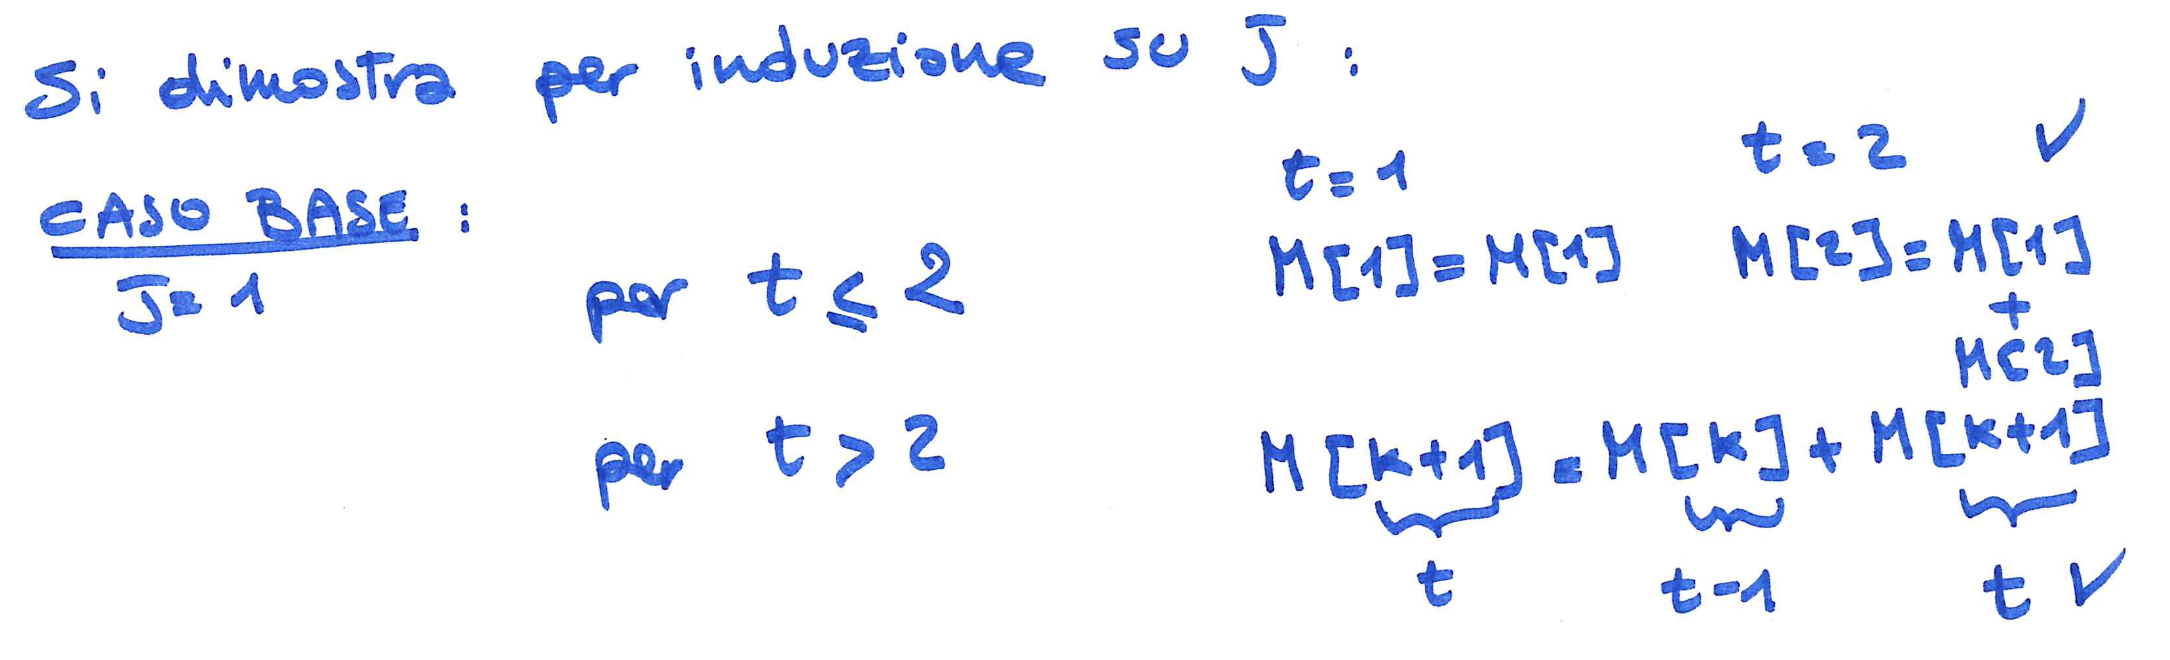
\includegraphics[scale=0.35]{images/dimostrazione_kogge_stone_caso_base.png}
    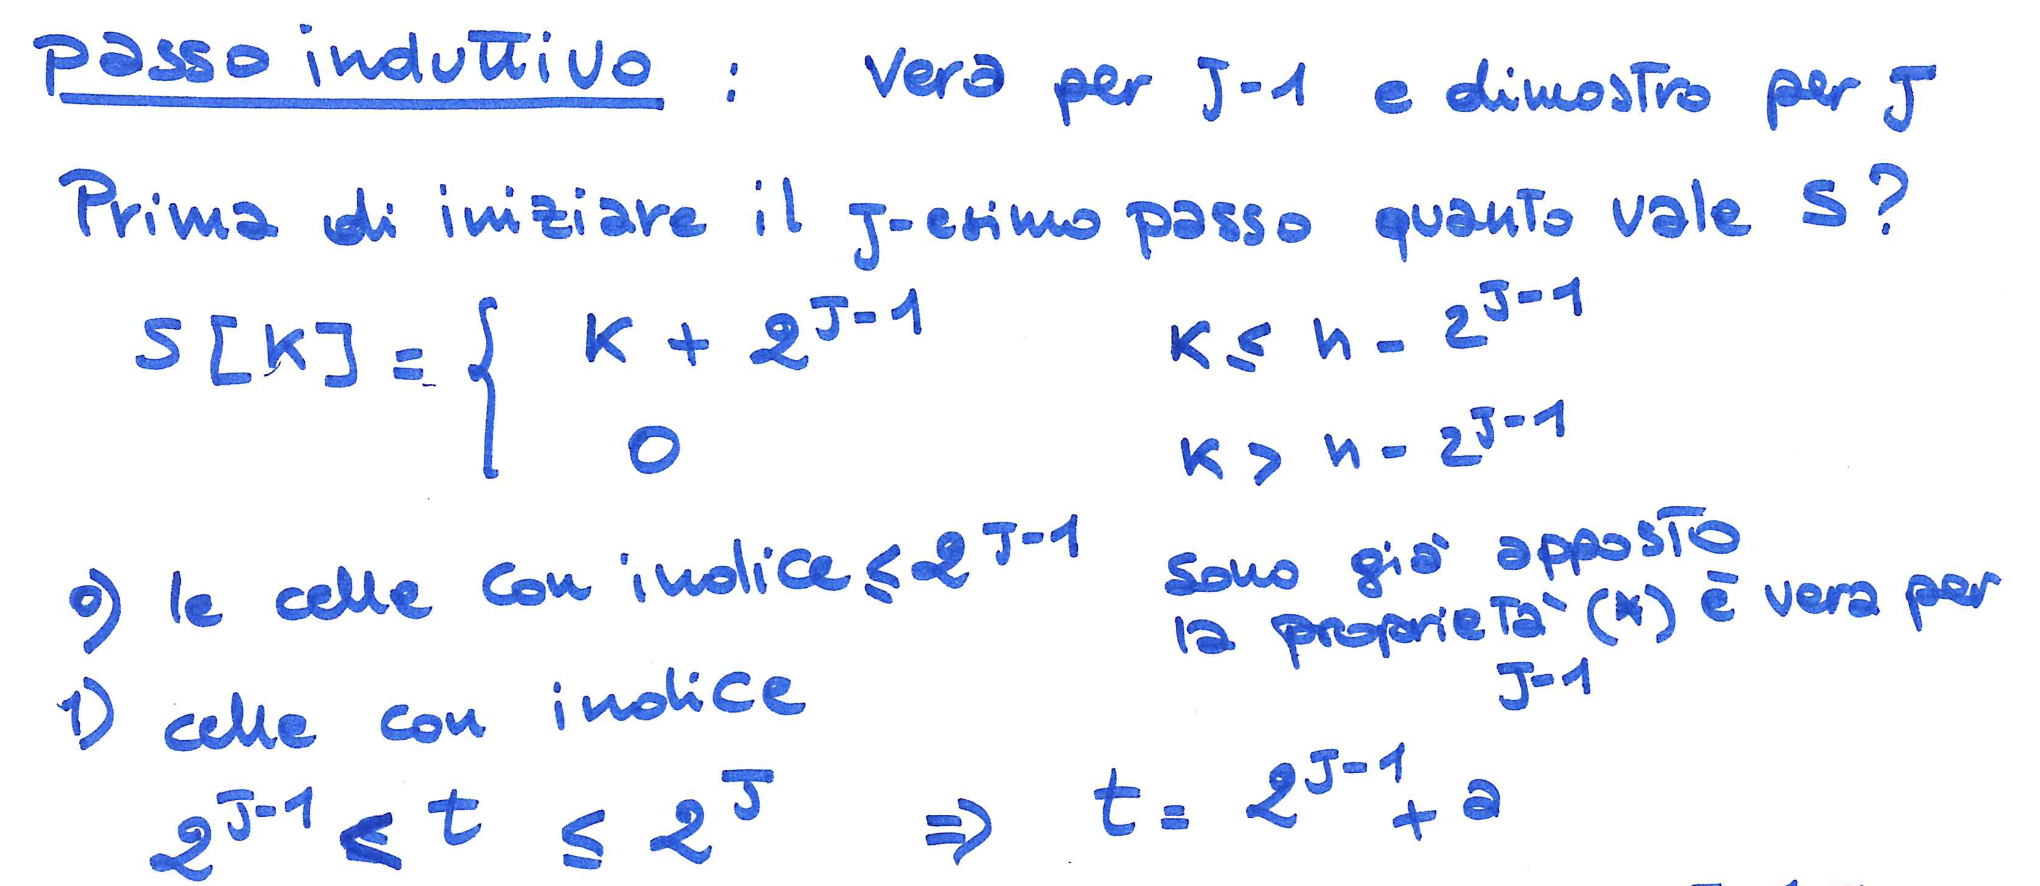
\includegraphics[scale=0.35]{images/dimostrazione_kogge_stone_caso_induttivo.png}
    \caption{Kogge Stone: dimostrazione}
\end{figure}

\begin{figure}[h]
    \centering
    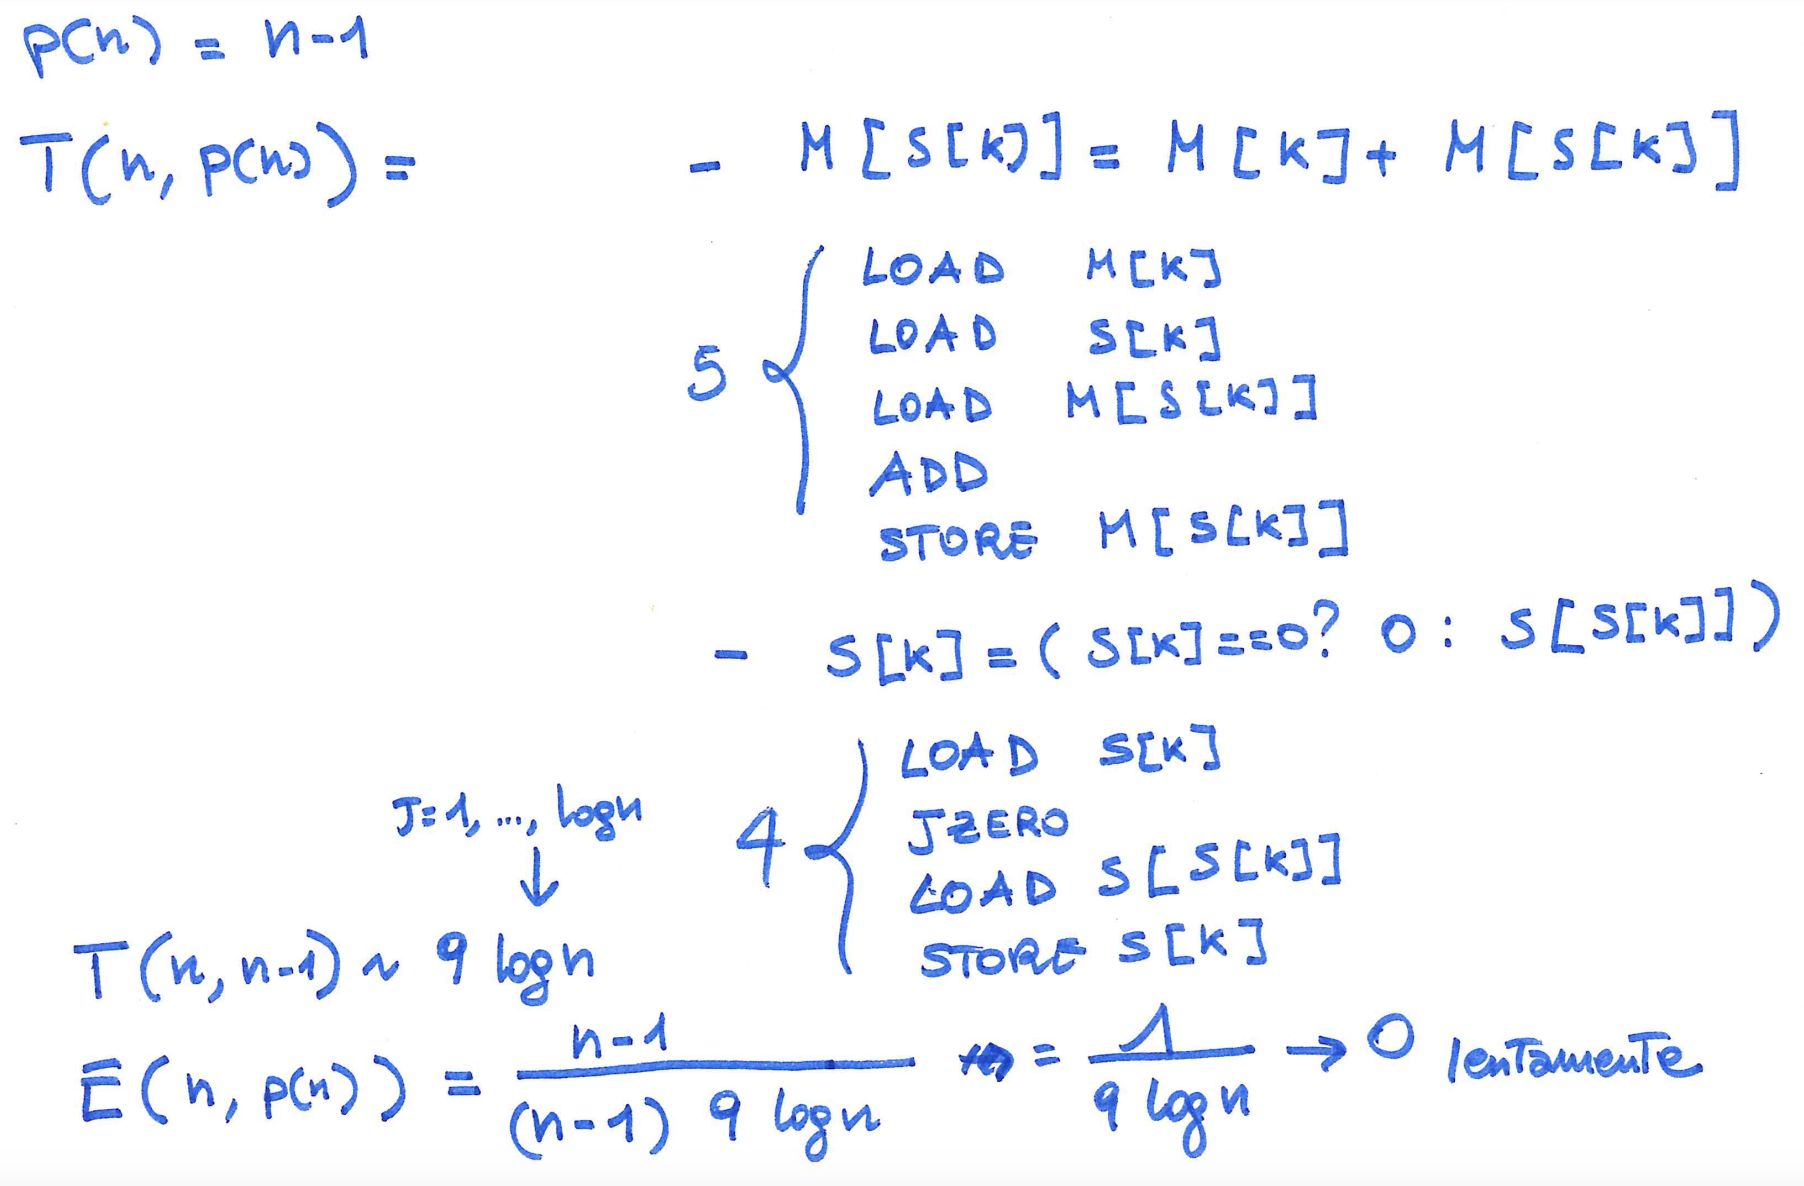
\includegraphics[scale=0.35]{images/valutazione_kogge_stone.png}
    \caption{Valutazione dell'algoritmo Pointer Doubling}
\end{figure}

\paragraph{Sfruttiamo Wyllie come per sommatoria}
Proviamo a raggruppare i processori di $\log n $ in $\log n$ in modo da far sparire la funzione $\log n$ da E
$$p(n) = o(\frac{n}{\log n})\;\;;\; T(n,p(n)) = O(\log n)\;\; ; \; E \rightarrow C \neq 0$$

\begin{comment}
\subsubsection{OP prefissa}
Come per sommatoria anche l'algoritmo dato per somme-prefisse può essere usato per OP-prefissa, dove OP \uline{deve essere associativa}. 

\paragraph{Valutazione dei polinomi}
Sfrutteremo come modulo l'operazione OP-prefissa.

Input: $p(x) = a_0 + a_1x + a_2x^2 + \dots + a_n x^n\; , \; \alpha$\\
Output: $p(\alpha)$

Alle $x$ va sostituito $\alpha$, si eseguono le operazioni sia di potenze che il prodotto con i coefficienti che la somma tra i vari monomi ottenuti.

Dati in memoria condivisa M:
\begin{itemize}
    \item il valore $\alpha$. E' un valore in una cella della memoria
    \item $a_0 + a_1x + \dots + a_n \rightarrow A[0], A[1], \dots , A[n]$. Il polinomio è specificato attraverso i coefficienti $A[i]$ in un vettore della memoria condivisa che chiamiamo $A$
\end{itemize}
Oltre al valore $\alpha$ abbiamo l'input. Le celle dove mettiamo i nostri coefficienti le chiamiamo A.

\paragraph{Algoritmo tradizionale sequenziale}
\begin{itemize}
    \item Numero di prodotti $\appprox n^2$
    \item Numero di somme $n$
\end{itemize}

In buona sostanza, un algoritmo sequenziale efficiente mi richiede $n^2$ operazioni, quindi un tempo quadratico

\paragraph{Miglioramento di Ruffini-Horner (caso sequenziale)}
\uline{Ci porta da un tempo quadratico ad uno lineare, precisamente $2n$}.
L'idea è quella di raccogliere $x$ in maniera iterata

\begin{figure}[h]
    \centering
    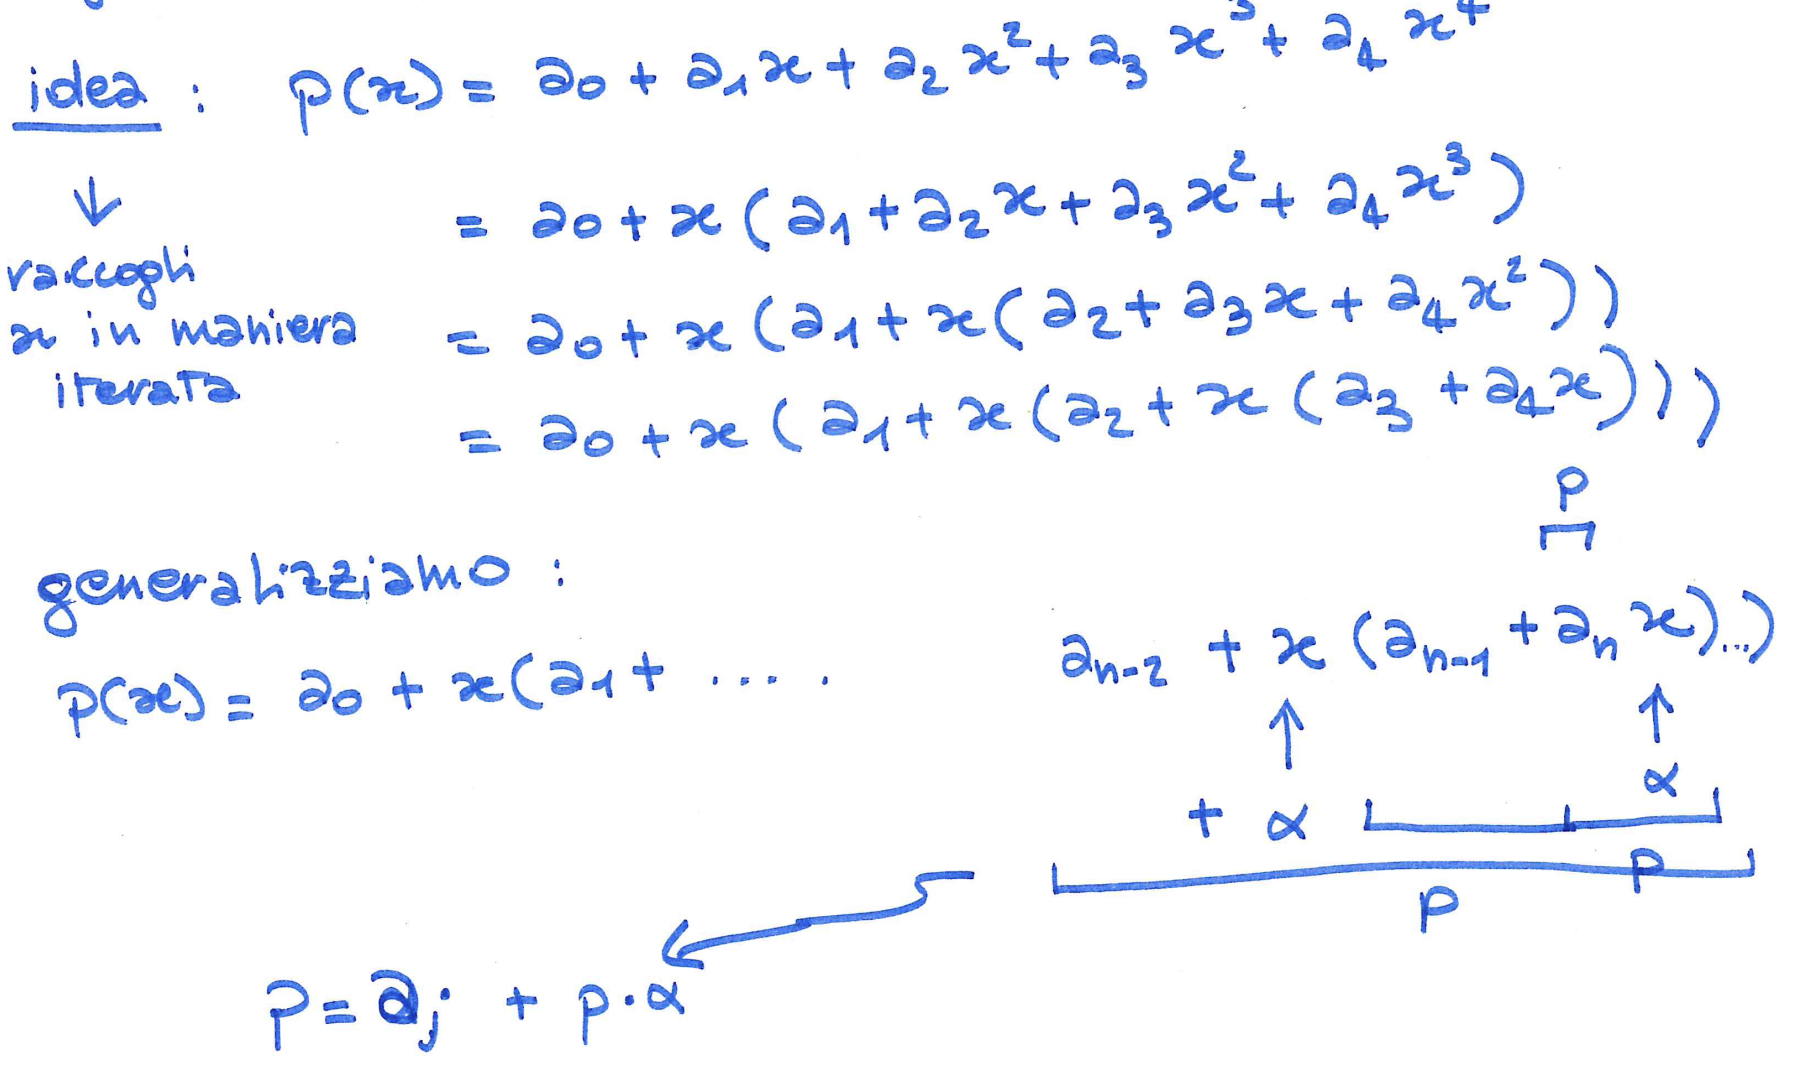
\includegraphics[scale=0.35]{images/ruffini_horner.png}
    \caption{Miglioramento di Ruffini-Horner caso sequenziale}
\end{figure}

Questa nuova forma del polinomio suggerisce un algoritmo, si può prendere una variabile $p$ che è il contenuto delle parentesi tonde. Ogni risultato viene rimesso in $p$

Inizializzo $p = an$, poi $p * \alpha + $ un coefficiente opportuno del mio polinomio e il risultato lo metto in $p$, che a sua volta sarà poi moltiplicato per $\alpha$ e sommato al coefficiente opportuno del polinomio.

L'istruzione $p = a_j + p * \alpha$ è un'istruzione che viene iterata all'interno di un ciclo for che fa variare $j$ opportunamente

\paragraph{Codice per algoritmo sequenziale Ruffini Horner}
\begin{lstlisting}
    Input(alpha)
        p = an
            for i = 1 to n
                p = an-i + p*alpha
    Output(P)
\end{lstlisting}

\paragraph{Prestazioni}
$$T(n,1) = 2n$$
Dobbiamo trovare un algoritmo parallelo che confrontato con questo tempo lineare risulta essere efficiente

\paragraph{Possibile algoritmo parallelo}
\begin{enumerate}
    \item 
    \begin{itemize}
        \item Costruisco il vettore delle potenze di $\alpha\; : \; Q$
        $$Q[K] = \alpha^K\;\;\; 0 \leq K \leq n$$
        E' un vettore nella memoria condivisa dove $$Q[0]=1, Q[1]=\alpha, Q[2]=\alpha^2, Q[n]=\alpha^n$$ 
        \item Eseguo il prodotto interno $<A,Q>$
        $$<A,Q>\;=\sum_{k=0}^n\; A[K]*Q[K]$$
        Quindi valutare i singoli monomi su $\alpha$ e poi sommarli
        \item Restituisco $<A,Q>$, il risultato del prodotto interno 
    \end{itemize}
\end{enumerate}

Per risolvere il punto $(1)$
\begin{itemize}
    \item Metto $\alpha$ in tutti gli elementi di $Q$ da $1$ a $n$
    $$Q[1] = \alpha, Q[2] = \alpha, \dots, Q[n] = \alpha$$
    Non considero la cella $Q[0]$ che deve contenere $1$, poi deve contenere $\alpha$. \uline{Porre tutto ad $\alpha$ significa risolvere un problema che si chiama REPLICA}\footnote{Replicare un valore in ogni elemento di un array}. Se riesco a risolvere il problema replica posso applicare il prodotto prefisso
    \item Applico il PRODOTTO-PREFISSO su $Q$
    $$Q[1] = \alpha, Q[2] = \alpha^2, \dots, Q[n] = \alpha^n$$
    In $Q[2]$ devo fare il prodotto prefisso ed avrò $\alpha^2$, etc. etc, alla fine in $Q[n]$ avrò $\alpha^n$
\end{itemize}

\paragraph{Come risolvere REPLICA in parallelo}

\begin{enumerate}
    \item Utilizziamo una batteria di $n$ processori, ognuno dei quali si occupa di sistemare la cella Q di indice K per K che va da $1$ ad $n$. Quindi ogni processore si occupa di una cella e va ad inserire in questa cella il valore $\alpha$
    \begin{lstlisting}
        for k = 1 to n par do
            Q[K] = alpha;
    \end{lstlisting}
    Questo algoritmo parallelo \uline{non è EREW} perchè abbiamo una lettura simultanea concorrente, se ogni processore si occupa della cella $Q[K]$ e su questo non c'è problema perchè ogni cella è dedicata ad un processore, il problema ce lo abbiamo su $\alpha$. Quando devono caricare $\alpha$ in $Q[K]$ tutti i processori si contendono $\alpha$, avviene una lettura simultanea essendo $\alpha$ in una cella di M condivisa.

    \uline{Questo codice va bene in una architettura CREW}

    Prestazioni di questo algoritmo
    $$p = n \;\; ; \;\; t = 2 \;\; ; \;\; E \approx \frac{n}{n*2} \rightarrow C \neq 0$$
    
    \item 
    \begin{lstlisting}
        for k = 1 to n/logn par do
            for i = 1 to log n do 
                Q[(k - 1) logn + i] = alpha 
    \end{lstlisting}

    Prestazioni di questo algoritmo:
    $$p = \frac{n}{\log n}\;\; ; \;\; t = c \log n \;\; ; \;\; E = \frac{n}{\frac{n}{\log n}\; c \; \log n = \frac{1}{c} \neq 0}$$ 

    Anche in questo caso abbiamo un algortimo CREW, per cui non abbiamo eliminato l'accesso simultaneo ad $\alpha$

    \item Desideriamo un EREW - PRAM, un replica EREW
    \begin{itemize}
        \item costruisci il vettore $\alpha, 0, 0, \dots , 0$ per poi fare che $\alpha$ venga copiato in ognuno di questi zeri. In questo modo avremmo risolto replica. Come è possibile mettere $\alpha$? Passo $2)$
        \item esegui SOMME-PREFISSE
    \end{itemize}

    Questo mi permette di eliminare la lettura concorrente di $\alpha$

    \begin{lstlisting}
        Input(alpha)
        Q[1] = alpha
        for k = 2 to n par do 
            Q[K] = 0
    \end{lstlisting}
    $0$ è una costante che non ha bisogno di essere letta

    
    Ho usato $n$ nel codice ma posso utilizzare \textit{Wyllie} che mi fa passare da $n$ processori a $\frac{n}{\log n}$ processori. Da un tempo costante ad un tempo logaritmico

    Prestazioni di questo algoritmo:
    $$p = \frac{n}{\log n}\;\; ; \;\; t = \log n$$
\end{enumerate}

\begin{figure}[h]
    \centering
    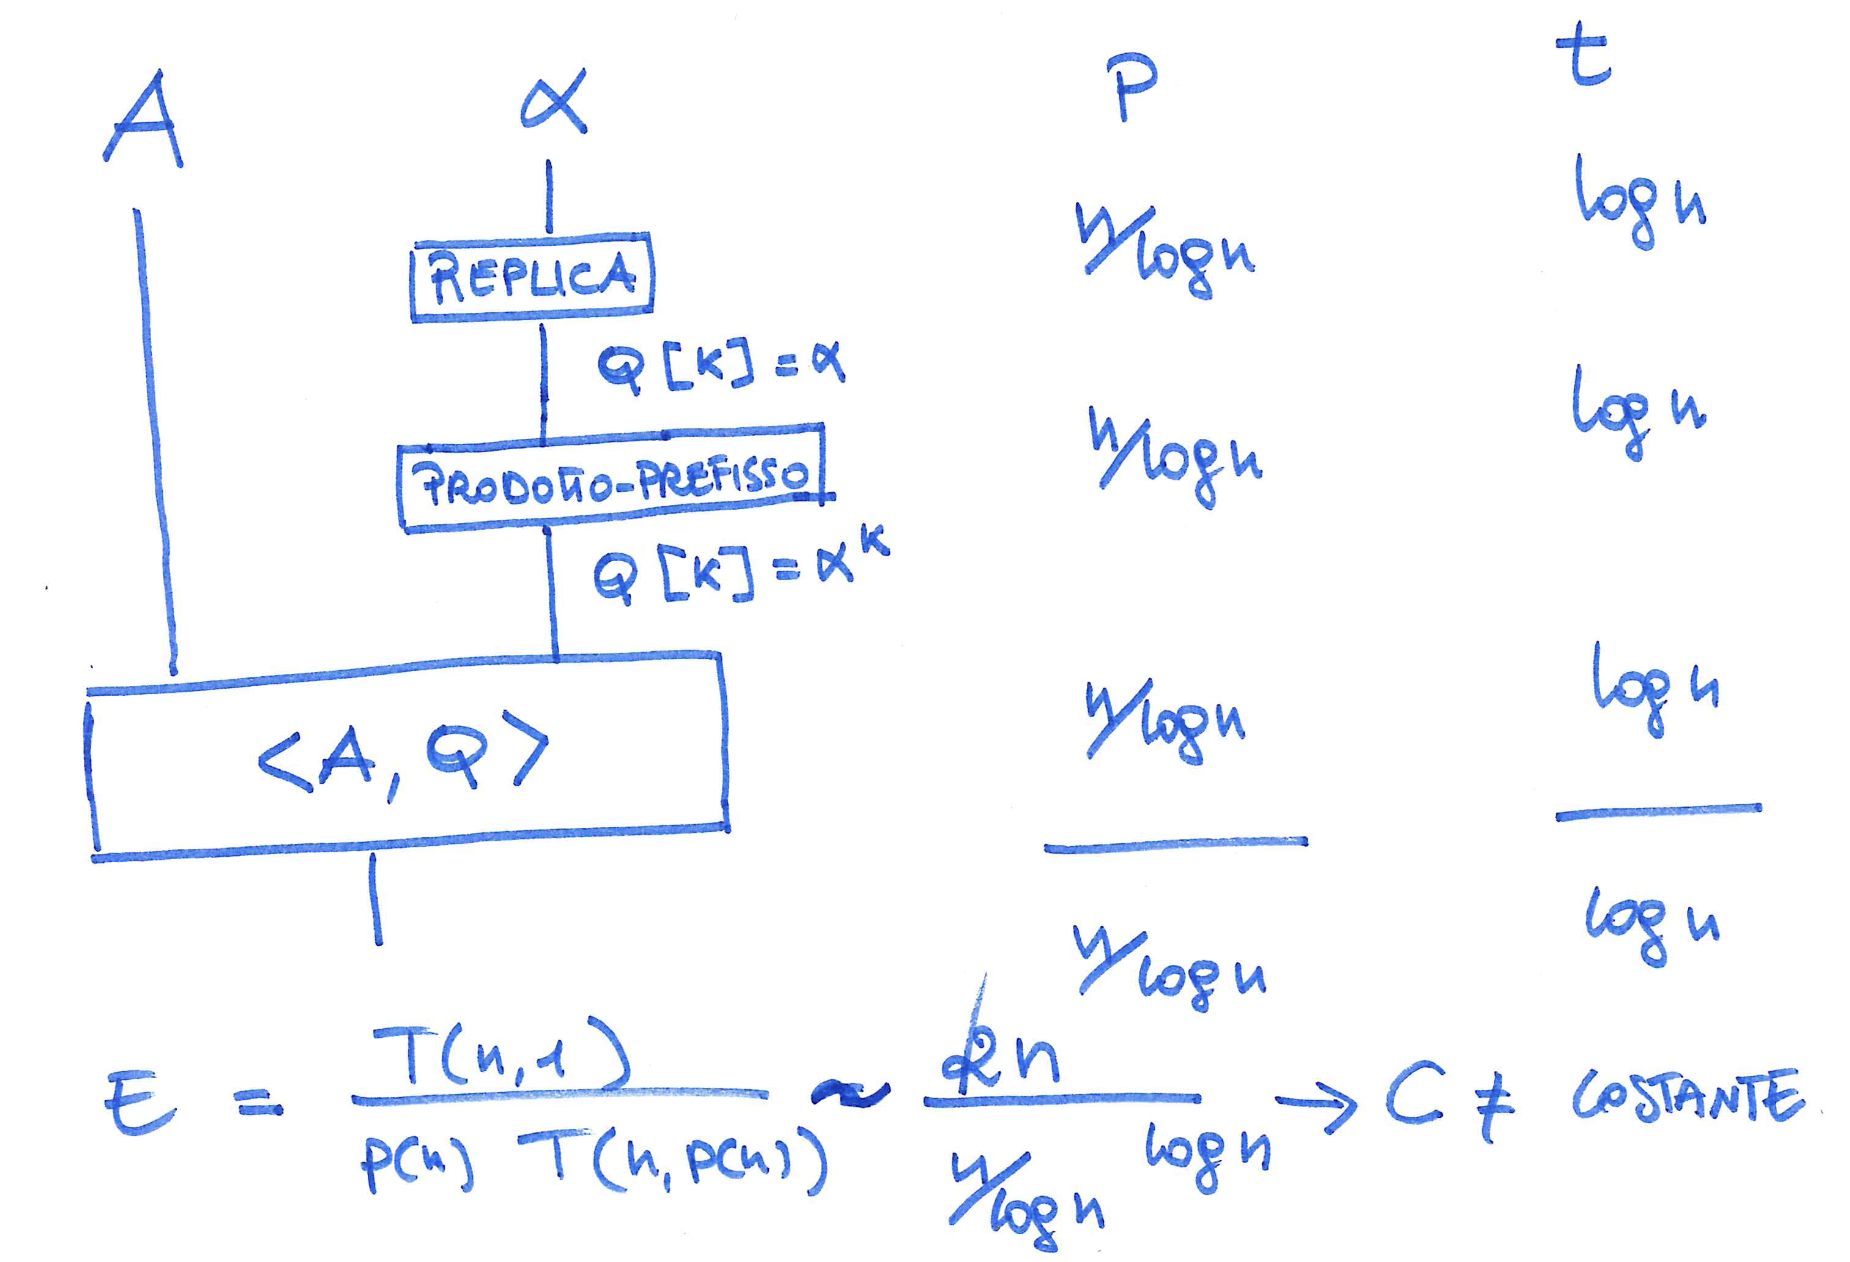
\includegraphics[scale=0.4]{images/valutazione_polinomio_erew_pram.png}
    \caption{Valutazione polinomio EREW PRAM}
    \label{fig:my_label}
\end{figure}
\end{comment}

\newpage


\subsection{Ricerca di un elemento}
Input: $M[1], M[2], \dots , M[n]$\\
Output: $M[n] = 1\; se\; \exists\; k \; t.c. \; M[k] = \alpha$ altrimenti $= 0$

Quando scopro che c'è il valore che sto ricercando vado a posizionare $1$ nella cella $M[n]$. E' una scelta di codice che potrebbe essere infelice se dopo una ricerca ne faccio un'altra.

\paragraph{Algoritmo sequenziale classico}
Richiede $n$ passi, $t = n$. Se l'input è ordinato posso migliorare ad un tempo logaritmico attraverso la ricerca dicotomica.

\paragraph{Algoritmi paralleli per ricerca}
\begin{enumerate}
    \item Proponiamo un algoritmo sull'architettura CRCW. Si utilizzano le celle della memoria M, si usa l'elemento $\alpha$ che è l'elemento da cercare che è input e sta nella memoria condivisa e si utilizza anche un \uline{flag}, anch'esso nella memoria condivisa

    \begin{minted}
    [
    frame=lines,
    framesep=2mm,
    baselinestretch=1.2,
    bgcolor=white,
    fontsize=\footnotesize,
    linenos
    ]{python}
    F = 0
    for k in range(1, n + 1):
        if M[k] == alpha:
            F = 1
    M[n] = F
    \end{minted}

    Se $M[n]$ è uguale a $1$ posso dire di avere trovato $\alpha$ nel mio vettore? Il problema è che non potendo inizializzare $M[n]$ a $0$ (perchè l'n-esimo processore deve accedervi e testare se c'è un valore uguale ad $\alpha$), non posso sapere se $1$ è la soluzione al problema o proprio il contenuto della cella

    Prestazioni di questo algoritmo: $p = n \; , \; t = \text{costante}$

    \item Su architettura CREW, cerca di eliminare la scrittura concorrente. Significa eliminare il flag.

    Trasformiamo il nosto vettore M in un vettore booleano che contiene $1, 0$. Quando una cella contiene $\alpha$ faccio scrivere valore $1$, altrimenti $0$. Dopodichè voglio spostare il risultato nella cella di indice maggiore e posso fare un \textit{MAX-ITERATO} che sposta l'$1$ (se c'è) nell'ultima cella del vettore $M[n]$

    \begin{minted}
    [
    frame=lines,
    framesep=2mm,
    baselinestretch=1.2,
    bgcolor=white,
    fontsize=\footnotesize,
    linenos
    ]{python}
    for k in range(1, n + 1):
        M[k] = 1 if M[k] == alpha else 0
    
    MAX_ITERATO(M[1], ..., M[n])
    \end{minted}

    Prestazioni di questo algoritmo: $p = n \; , \; t = \text{costante}$

    \item Su architetture EREW
    \begin{minted}
    [
    frame=lines,
    framesep=2mm,
    baselinestretch=1.2,
    bgcolor=white,
    fontsize=\footnotesize,
    linenos
    ]{python}
    REPLICA alpha -> A[1], A[2], ..., A[n]
    for k in range(1, n + 1):
        M[k] = 1 if M[k] == A[k] else 0
    
    MAX_ITERATO(M[1], ..., M[n])
    \end{minted}

    Con questo semplice accorgimento della replica abbiamo risolto il problema della concurrent read. Mi ha consentito di passare da un CRCW ad un EREW
    
    Prestazioni di questo algoritmo:\\
    $$p = \frac{n}{\log n}\;\; ; \;\; t = \log n \; \implies E = C \neq 0$$
    
\end{enumerate}

\newpage


\subsection{Ordinamento}
Abbiamo una sequenza di interi e la vogliamo ordinare. Formalmente \textit{RANKING}. 

Input: $M[1], \dots , M[n]$\\
Output: permutazione : $P:{1, \dots, n} \rightarrow {1, \dots , n}$ t.c. $M[P(1)] \leq M[P(2)] \leq \dots \leq M[P(n)]$

dove $p(i)$ è l'indice dell'elemento del vettore M che va in posizione i 

\begin{osservazione}
    In genere gli algoritmi di ordinamento sono basati sui CONFRONTI. Gli algoritmi di ordinamento che usano i confronti hanno un tempo $t = \Theta (n \log n)$. Questo è sia un \textit{upper bound} che un \textit{lower bound}. Upper bound perchè esistono algoritmi come il Merge Sort\footnote{Il Merge sort è un algoritmo di ordinamento che funziona dividendo ricorsivamente una serie di elementi in sottoserie sempre più piccole, fino a quando ogni sottoserie non contiene più di un elemento. A quel punto, le sottoserie vengono ricombinate in ordine crescente, unendo due sottoserie ordinate alla volta, fino a ottenere l'array ordinato finale} che impiega $n \log n$ passi e lower perchè si può dimostrare che se l'algoritmo è basato sui confronti meno di $n \log n$ passi non possiamo fare.
\end{osservazione}

\paragraph{Dimensione di lower bound}
Tutto si basa sull'utilizzo nella dimostrazione di un albero di decisione. \uline{Qualsiasi algoritmo che si basa su confronti durante l'esecuzione produce un albero di decisione, o meglio, un cammino all'interno dell'albero di decisione}. L'albero di decisione è l'algoritmo in sè.

E' un albero binario. \uline{Sui nodi abbiamo i confronti} e ha un figlio sinistro e uno destro. Se al confronto la risposta è positiva si scende verso sinistra, altrimenti a destra.

\uline{Le foglie dell'albero di decisione rappresentano la permutazione dell'input p}. Tale permutazione è conseguenza delle risposte e quindi dei confronti che abbiamo fatto e dimostra come l'input deve essere permutato per ottenerlo ordinato. Cioè ogni foglia individua un cammino, questo cammino sono le sequenze di passi che questo algoritmo mi ha fatto eseguire per poter ordinare il mio array.

\uline{L'altezza dell'albero rappresenta il tempo di esecuzione dell'algoritmo perchè l'altezza di un albero rappresenta il cammino più lungo all'interno del mio albero binario}. Il cammino più lungo equivale al caso peggiore, il massimo numero di passi che devo fare per permutare il mio input

\begin{osservazione}
    Il numero di foglie deve essere almeno $n!$, perchè devono prevedere tutti i possibili ordinamenti di $n$ elementi. Se $t$ è l'altezza il numero massimo di foglie è $2^t$ da cui si ricava che
    $$2^t \geq \#foglie \geq n! \implies t \geq \log n$$
\end{osservazione}

\subsubsection{Counting sort}
Un algoritmo basato sul conteggio e richiede un tempo $t = \Theta(n^2)$

Assumiamo che $n$ sia potenza di $2$ con elementi tutti diversi tra loro.

\uline{Useremo un vettore per salvare le posizioni delle celle ed ottenere l'array ordinato}. Perciò se $M[i]$ va in $k$, metterò in $V[i] = k$. 

$V[i]$ mi dice la posizione finale dell'elemento $i$ del vettore. Questa definizione di $V[i]$ mi da la permutazione inversa che io sto cercando

\paragraph{Counting sort sequenziale}.

\begin{minted}
[
frame=lines,
framesep=2mm,
baselinestretch=1.2,
bgcolor=white,
fontsize=\footnotesize,
linenos
]{python}
for i in range(1, n + 1):
    V[i] = 0

for i in range(1, n + 1):
    for j in range(1, n + 1):
        if M[j] <= M[i]:
            V[i] += 1

F = [0] * (n + 1)
for i in range(1, n + 1):
    F[V[i]] = M[i]

for i in range(1, n + 1):
    M[i] = F[i]
\end{minted}

Se vogliamo restituire il vettore V (la permutazione) l'algoritmo termina al secondo for, se vogliamo invece M ordinato continua

\paragraph{Versione parallela} 
Si cerca di rendere parallelo un algoritmo sequenziale già noto
\begin{enumerate}
    \item Possiamo pensare di prendere un numero di processori $n^2$ per ogni $i, j$ e ogni processore esegue il confronto $M[j] \leq M[i]$. Invece di eseguire la fase 2) (il secondo for) in modo sequenziale, utilizziamo un processore per ogni confronto e mettiamo la risposta in una \uline{matrice booleana} $V[i,j]$
    \begin{lstlisting}
        V[i,j] = (M[j] <= M[i] ? 1:0)
    \end{lstlisting}
    
    Cosa rappresenta la i-esima riga della matrice booleana? Individua gli elementi di $M \leq M[i]$. Contando gli $1$ della riga, so quanti elementi sono $\leq M[i]$ 

    \item \uline{Se per ogni $i$ eseguo la sommatoria parallela della i-esima riga}, ottengo nell'ultima colonna della matrice le posizioni che devono assumere i miei elementi $M[i]$. Sto sommando tutti gli $1$ della riga e li sto mettendo nell'ultimo elemento della prima riga
\end{enumerate}


\paragraph{Codice}.

\begin{minted}
[
frame=lines,
framesep=2mm,
baselinestretch=1.2,
bgcolor=white,
fontsize=\footnotesize,
linenos
]{python}
for i in range(1, n + 1):
    for j in range(1, n + 1):
        V[i,j] = 1 if M[j] <= M[i] else 0

for i in range(1, n + 1):
    SOMMATORIA = sum(V[i, j] for j in range(1, n + 1))

for i in range(1, n + 1):
    M[V[i, n]] = M[i]
\end{minted}

Abbiamo $n^2$ processori e ognuno fa confronti su $j,i$. Siccome questi processori fanno confronti in parallelo gli indici $i,j$ vengono utilizzati $n$ volte. Quindi \uline{la lettura di questi elementi non è esclusiva per processore ma è una lettura simultanea}. \uline{Non possiamo dire che il nostro algoritmo è EREW}.

Per la scrittura diciamo che ogni processore ha la sua cella dove scrive quindi sicuramente non c'è concorrenza sulla scrittura.

\paragraph{Algoritmi di ordinamento paralleli}
\begin{itemize}
    \item Counting-sort 
    $$E = \frac{\log n}{n} \rightarrow 0$$
    \item Bit-sort 
    $$E = \frac{1}{\log n} \rightarrow 0$$
    E' un buon algoritmo parallelo che però non ha ancora un'efficienza costante, ha un'efficienza che tende a zero anche se ci tende lentamente 
\end{itemize}

\subsubsection{Bitonic sort}
Prende spunto dal \textit{Merge sort} ma mette in gioco nuove idee, in particolare nuove sequenze chiamate \uline{unimodali} e \uline{bitoniche}. Il nome deriva appunto da bitoniche, perciò bit-sort (bitonic-sort)

\paragraph{Algoritmo Merge Sort sequenziale}
Utilizza la \uline{tecnica divide et impera}, prende cioè un array di lunghezza $n$ e lo divide richiamando se stesso in due metà. \textit{Merge} fonderà due array già ordinati

\begin{minted}
[
frame=lines,
framesep=2mm,
baselinestretch=1.2,
bgcolor=white,
fontsize=\footnotesize,
linenos
]{python}
if len(A) > 1:
    As = Mergesort(A[0:n//2])
    Ad = Mergesort(A[n//2:])
    A = Merge(As, Ad)
return A
\end{minted} 

Questo \textit{MergeSort} viene chiamato ricorsivamente fino ad ottenere un unico elemento. Nel caso peggiore ogni elemento viene confrontato con due elementi dell'altro array. Perciò $t = n$ nel caso peggiore

Tempo di Merge-sort:\\
\begin{equation}
    t(n) = 
        \begin{cases}
            0 & \text{n=1, ritorna A}\\
            2t(\frac{n}{2})+n  & \text{altrimenti}
        \end{cases}
\end{equation}

\begin{figure}[h]
    \centering
    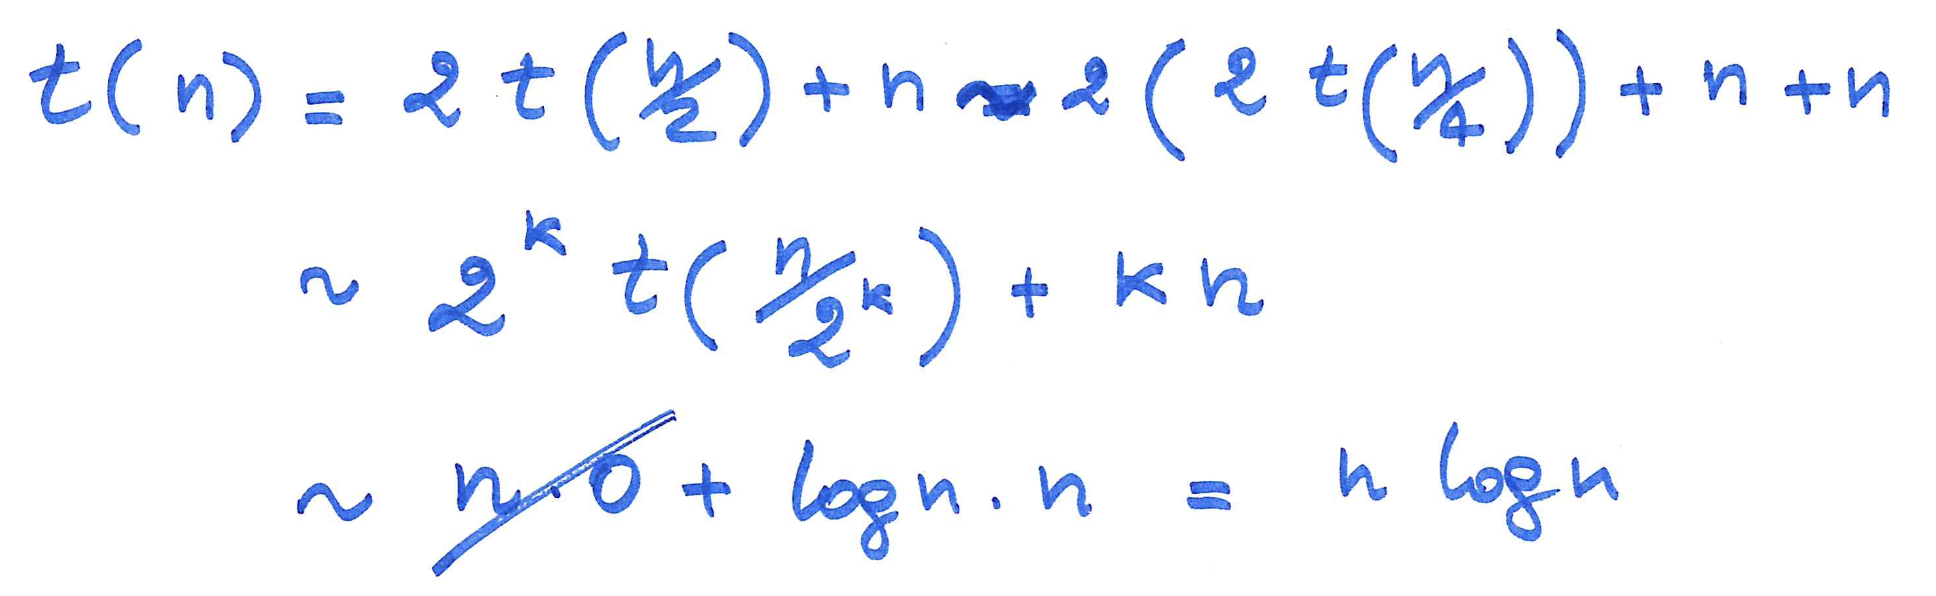
\includegraphics[scale=0.35]{images/merge_sort_tempo.png}
\end{figure}

Se usassi un parallelo quello che mi costa è l'operazione di merge, la divisione dell'input non mi costa niente. Purtroppo il \textit{Merge} non è parallelizzabile, lo devo tenere così com'è e ottengo ancora $T \approx n \log n$

Al posto di chiedersi qual'è il caso peggiore. Quando \textit{Merge} è facile?  

E' facile quando gli elementi di $A_s$ sono tutti minori di $A_d$, in questo caso basta concatenare i due array.
\uline{Dobbiamo cercare di trasformare il nostro input in modo che il Merge faccia questa semplice operazione}

Da qui nasce l'idea per un buon algoritmo parallelo che fa uso di particolari sequenze numeriche che si chiamano \textbf{UNIMODALI} e \textbf{BITONICHE}. Oltre a queste abbiamo bisogno anche di ulteriori routine \uline{REV} e \uline{MIN MAX}. Queste sono funzioni richiamate dal \textit{bit-sort} per cui saranno effettuate in parallelo

\paragraph{Funzione REV}
Fa il reverse di un array. Si leggono i valori $A[1]$ e $A[n]$ e si scambiano di posizione. Si swappano coppie di elementi, che inizialmente sono il primo e l'ultimo e poi si passa al secondo e al penultimo.

Algoritmo parallelo:
\begin{minted}
[
frame=lines,
framesep=2mm,
baselinestretch=1.2,
bgcolor=white,
fontsize=\footnotesize,
linenos
]{python}
for k in range(1, n//2 + 1):
    A[k], A[n - k + 1] = A[n - k + 1], A[k]
\end{minted}

Fa lo swap degli elementi a pari distanza rispetto al centro.

Siccome le coppie sono $\frac{n}{2}$, avrò processori $p = \frac{n}{2}$. Tempo costante

\paragraph{Funzione MIN-MAX}
Permette di costruire gli array $A_{min}$ e $A_{max}$.\\
Considera sempre l'array in due metà, confronta gli elementi a coppie prendendo un elemento della prima metà e uno della seconda metà. In particolare gli elementi devono essere a distanza $\frac{n}{2}$. Da questi confronti vengono fuori il minimo e il massimo. Gli elementi della prima metà $A_{min}$ contengono i minimi, gli elementi della seconda metà $A_{max}$ contengono i massimi

Algoritmo parallelo:
\begin{minted}
[
frame=lines,
framesep=2mm,
baselinestretch=1.2,
bgcolor=white,
fontsize=\footnotesize,
linenos
]{python}
for k in range(1, n//2 + 1):
    if A[k] > A[k + n//2]:
        A[k], A[k + n//2] = A[k + n//2], A[k]
\end{minted}

Anche in questo caso impiego $p = \frac{n}{2}$ processori. Lo SWAP costa $4$, qui c'è un confronto (quindi una micro-istruzione in più). Il tempo è dato da $5$ micro-istruzioni. \uline{Tempo costante}

\paragraph{Particolari sequenze numeriche}
\begin{itemize}
    \item UNIMODALE\\
    Una sequenza è detta unimodale sse $\exists\; k$ che fa da elemento minimo della sequenza per cui da $1$ fino a $k$ i miei elementi decrescono, da $k$ fino ad $A[n]$ i miei elementi crescono. Quindi ho un minimo che è l'elemento $A[K]$.

    Esiste una posizione tale per cui la mia sequenza cresce e poi decresce 
    $$A[1] > A[2] > \dots > A[K] < A[K+1] < \dots$$
    Oppure è vero il viceversa
    $$A[1] < A[2] < \dots > A[K] > A[K+1] > \dots$$
    $A[K]$ invece di essere un minimo è un massimo. Gli elementi decrescono fino ad arrivare a $k$ e poi crescono. \uline{Parzialmente ordinata}
    \item BITONICA\\
    Una sequenza è detta bitonica quando \uline{può essere trasformata in una sequenza unimodale mediante una permutazione ciclica di se stessa}.

    Cioè esiste un $j$ tale per cui prendendo gli elementi da $A[j]$ fino ad $A[n]$ concatenato ad $A[1]$ fino ad $A[j-1]$ ho una sequenza unimodale.

    Ho preso un suffisso della sequenza, l'ho reso un prefisso della sequenza ed ho trasformato in una unimodale, ora esisterà un $k$ che sarà valore minimo o massimo
\end{itemize}

\begin{figure}[h]
    \centering
    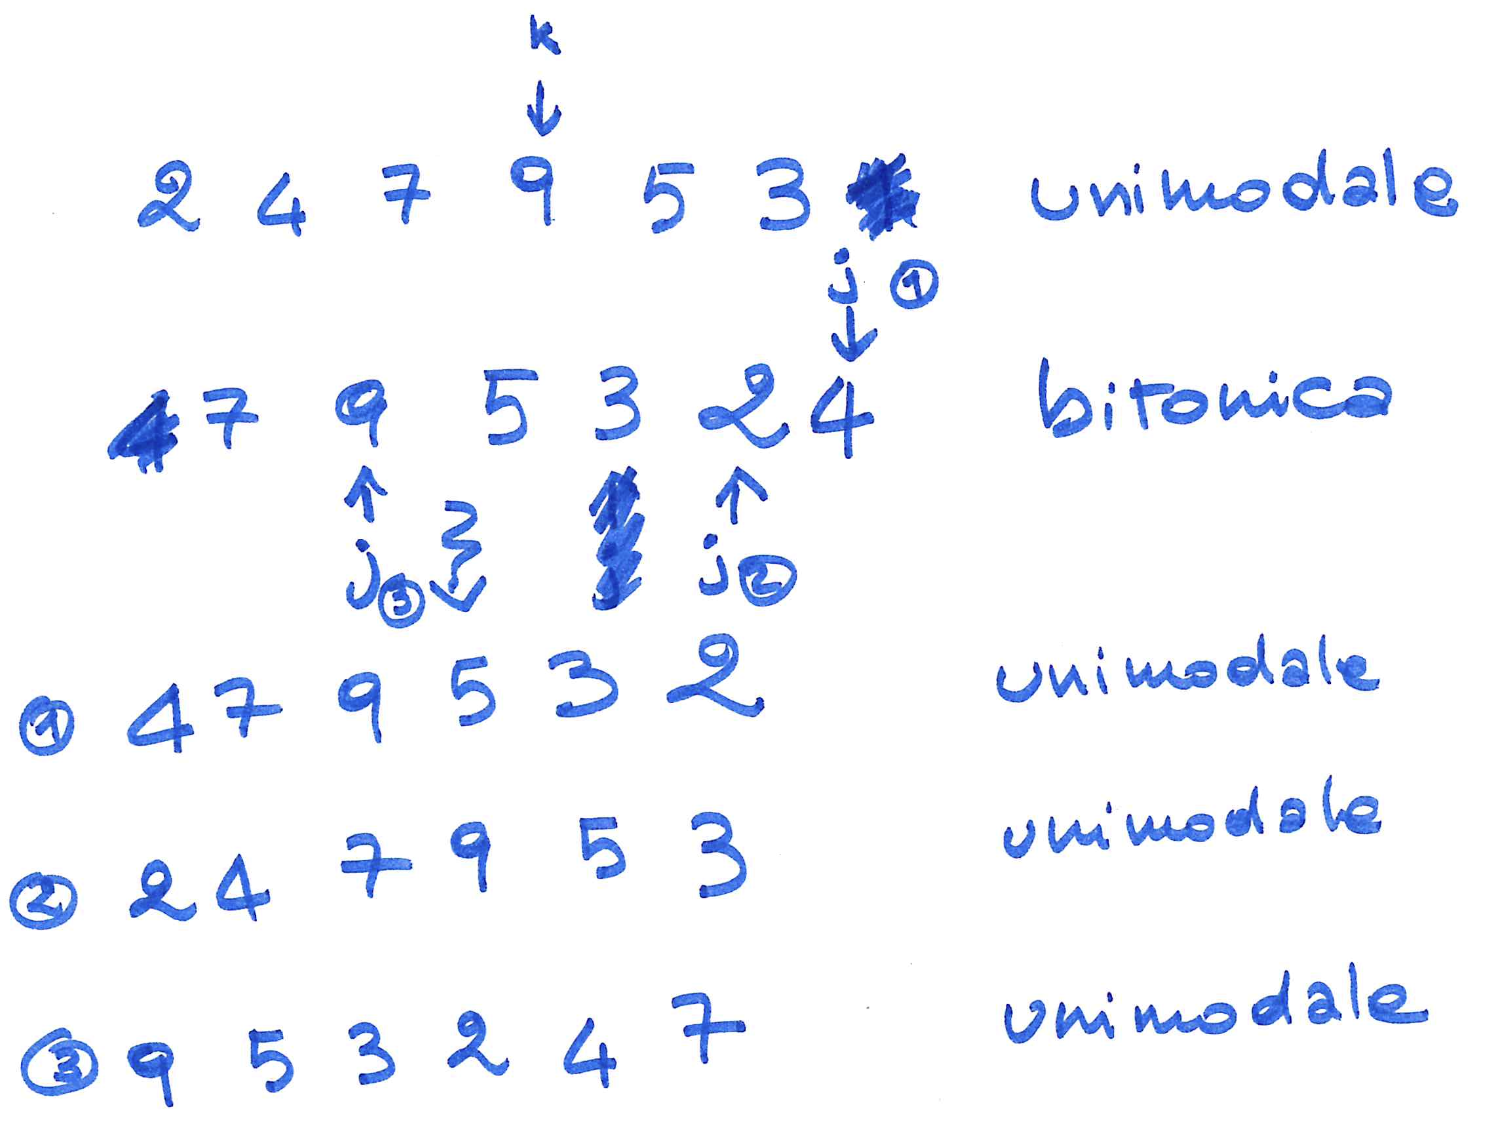
\includegraphics[scale=0.4]{images/bitonica1.png}
\end{figure}

\begin{figure}[h]
    \centering
    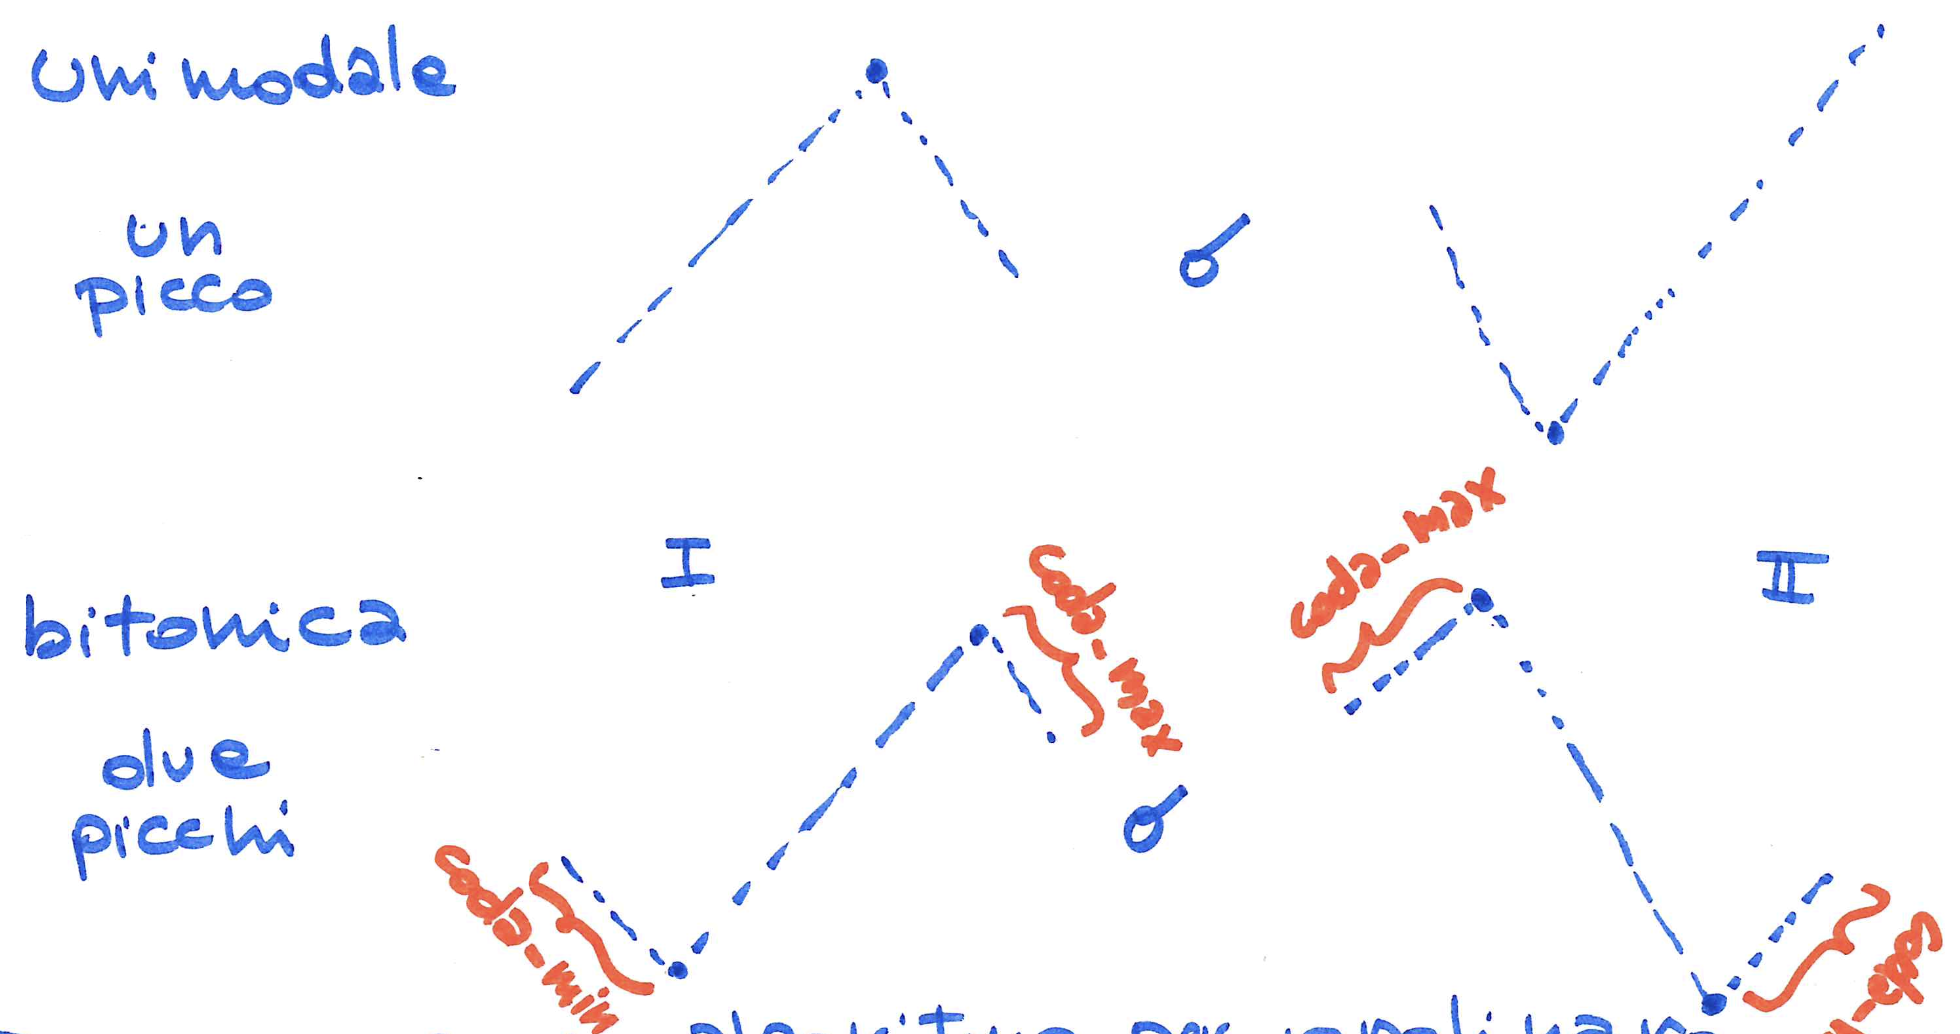
\includegraphics[scale=0.35]{images/bitonica2.png}
\end{figure}


I grafici sono ottenuti plottando gli elementi della sequenza sul piano. Posso spostare \textit{coda-min} e \textit{coda-max} in modo da traformare i due picchi in un picco, traformando così la bitonica in unimodale.

%Bit merge
\subsubsection{Bit merge}
\begin{osservazione}
    Se una sequenza è unimodale è anche bitonica
\end{osservazione}

\begin{osservazione}
    Siano $A, B$ due sequenze ordinate crescenti la sequenza $A * REV(B)$ è unimodale
\end{osservazione}

\paragraph{Proprietà} Se effettuo \textit{MIN-MAX} su una sequenza A
\begin{enumerate}
    \item $A_{min}$ e $A_{max}$ sono ancora bitoniche
    \item $A_{min}$ è fatto di elementi minori degli elementi di $A_{max}$
\end{enumerate}

Tali proprietà suggeriscono un approccio divide-et-impera:
\begin{enumerate}
    \item MIN-MAX suddivide il problema su $n$ elementi in istanze più piccole ($\frac{n}{2}$): $A_{min}$, $A_{max}$  grazie alla proprietà $1$
    \item Ordinando $A_{min}$ e $A_{max}$ la fusione (merge) avviene per concatenazione grazie alla proprietà $2$. Se sono ordinati l'array ordinato si ottiene banalmente concatenando
\end{enumerate}

\paragraph{Algoritmo sequenziale}:
\begin{minted}
[
frame=lines,
framesep=2mm,
baselinestretch=1.2,
bgcolor=white,
fontsize=\footnotesize,
linenos
]{python}
MIN_MAX(A)
if len(A) > 2:
    bit_merge(Amin)
    bit_merge(Amax)
return A
\end{minted}
\textit{bit-merge} ordina le sequenze bitoniche. Restituendo A ritorno due liste ordinate crescenti e concatenandole ottengo il risultato. Correttezza di bit-merge: Si utilizza l'induzione
\begin{itemize}
    \item Caso base: $n=2$\\
    Entro con un input di due elementi, \uline{dopo il MIN-MAX il vettore è ordinato}. Il minimo in prima posizione, il massimo in seconda. Una sequenza di lunghezza $2$ è banalmente ordinata da \textit{MIN-MAX}
    \item Passo induttivo\\
    Supponiamo che per $n = 2^k$ l'algoritmo sia corretto\\
    Dimostriamo che è valido per $A = 2^k + 1$\\
    $A_{min}$ e $A_{max}$ restituiti sono lunghi la metà, quindi $2^k$, vengono passati a \textit{bit-merge}. Abbiamo assunto (ipotesi induttiva) che per quell'ordine di lunghezza l'algoritmo è corretto quindi vengono fuori ordinati e la concatenazione lavora perchè gli elementi di $A_{min} < A_{max}$
\end{itemize}

\paragraph{Implementazione parallela}

%Image lesson 12 parte 2 26.35''

All'inizio c'è un unico \textit{MIN-MAX}, poi viene richiamato da \textit{bit-merge}. All'i-esimo passo mi aspetto i chiamate a \textit{MIN-MAX} su dimensione dell'input $\frac{n}{2^{i-1}}$ fino ad arrivare a \textit{MIN-MAX} effettuato a $2$ elementi, a quel punto si ferma la chiamata ricorsiva

\paragraph{Valutazione}
Lavora su dati diversi di input, perchè ogni volta divide l'input. Ogni \textit{MIN-MAX} lavora su input diversi perciò è EREW P-RAM.

\paragraph{Tempo}
Mi fermo quando $\frac{n}{2^{i-1}} = 2$ da cui ottengo che $i = \log n$. L'albero che disegnamo dove si esegue l'algoritmo parallelo ha profondità logaritmica.

\paragraph{Processori}
Il primo passo parallelo richiede $\frac{n}{2}$ processori. Il secondo passo ne richiede la metà per due $\frac{n}{4} + \frac{n}{4} = \frac{n}{2}$ etc. Quindi ogni passo sostanzialmente richiede $\frac{n}{2}$ processori. 

\paragraph{Efficienza}
$$E = \frac{n \log n}{\frac{n}{2} \; 5 \log n} \rightarrow C \neq 0$$
Sopra il tempo sequenziale di qualsiasi algoritmo che ordina una sequenza numerica. Sotto tempo parallelo. Abbiamo una costante diversa da zero perciò un algoritmo efficiente.


\paragraph{Bit-sort}
Batcher $1968$. Ordina non solo sequenze \textit{unimodali} e \textit{bitonica} e prende spunto dal \textit{bit-merge}

\begin{minted}
[
frame=lines,
framesep=2mm,
baselinestretch=1.2,
bgcolor=white,
fontsize=\footnotesize,
linenos
]{python}
MINMAX(A)
if len(A) > 2:
    bit_sort(Amin)
    bit_sort(Amax)
    bit_merge(Amin * REV(Amax))
return A
\end{minted}

Se entrambi sono ordinati, la fusione la faccio con \textit{bit-merge}, la trasformo in una sequenza unimodale che è anche bitonica. Il bit-merge non faceva la fusione

\paragraph{Correttezza di bit-sort}
Si utilizza l'induzione
\begin{itemize}
    \item Caso base $n=2$\\
    \textit{MIN-MAX} su due elementi li ordina
    \item Passo induttivo\\
    Suppongo che sia corretto per $2^k$ e dimostro che vale per $2^{k+1}$, quindi $|A| = 2^{k+1}$

    \begin{itemize}
        \item \textit{MIN-MAX} divide A in $A_{min}$ e $A_{max}$ di lunghezza $2^k$
        \item bit-sort($A_{min}$) e bit-sort($A_{max}$) li ordinano per ipotesi induttiva
        \item bit-merge($A_{min}\;REV(A_{max})$) ordina A
    \end{itemize}
\end{itemize}

\begin{figure}[h]
    \centering
    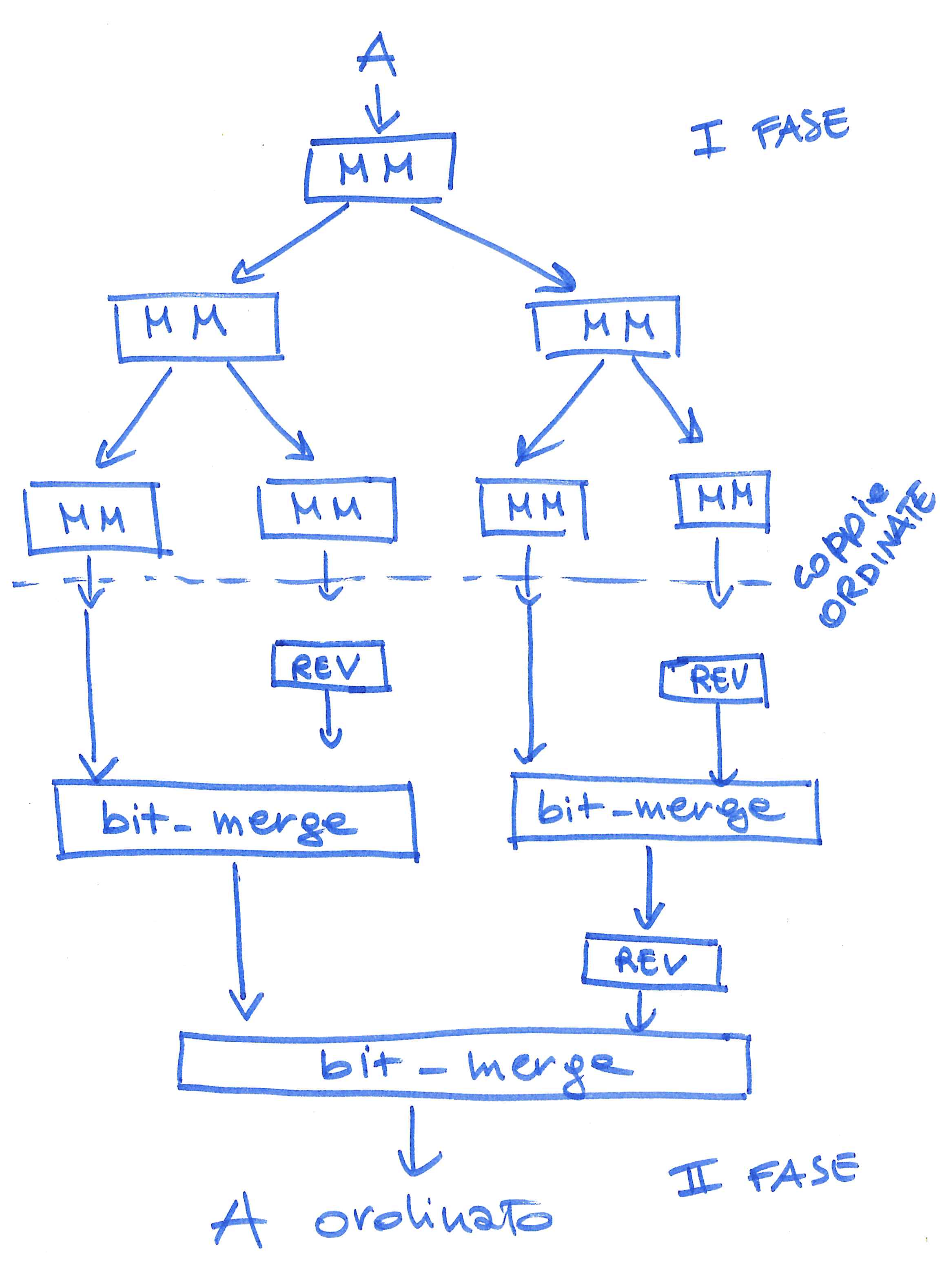
\includegraphics[scale=0.4]{images/bitsort_parallelo.png}
    \caption{Implementazione parallela di bit-sort}
\end{figure}

\paragraph{Valutazione dell'algoritmo}
Questo algoritmo come \textit{bit-merge} è EREW perchè dividiamo ogni volta l'input, non c'è intersezione sui dati su cui lavorano. 

\paragraph{Tempo}
\begin{itemize}
    \item I fase\\
    \textit{i} è l'ultimo passo. (come bit-merge) $i = \log n$. Si esegue MIN-MAX che richiede tempo costante $T(n) = O (\log n)$
    \item II fase\\
    \textit{i} è l'ultimo passo $i = \log n-1$. Si esegue REV costante e bit-merge che richiede $O (\log n) \text{, perciò} \; T(n) = O(\log^2 n)$
\end{itemize}

\paragraph{Processori}
MIN-MAX nella prima fase mi richiede $\frac{n}{2}$ processori, nella seconda fase ho REV e bit-merge, anche loro richiedono $\frac{n}{2}$ processori. Perciò $P = \frac{n}{2}$

%Image lesson 13 parte 1 37.00''

\paragraph{Efficienza}
$$E = \frac{n \log n}{\frac{n}{2}\;5\;\log^2n} \rightarrow \frac{\alpha}{\log n} \rightarrow 0 \;\text{lentamente}$$

\newpage


%Ciclo Euleriano
\subsection{Ciclo Euleriano}
Tecnica applicata in diversi contesti, serve per gestire strutture dati dinamiche. Gestire operazioni su alberi

\paragraph{Definizioni base di Teoria dei Grafi}
\begin{itemize}
    \item Un grafo diretto D è una coppia $(V,E)$ dove $E \in V^2$. Un grafo diretto ha un orientamento. Con la notazione $(\upsilon, \omega)$ denotiamo un arco uscente da $\upsilon$ ed entrante in $\omega$
    \item Cammino: è una sequenza di archi $e_1, e_2, \dots , e_i, e_{i+1}, \dots , e_k$ c'è una proprietà tra due nodi consecutivi tale che il nodo finale (pozzo) di $e_i$ coincide con il nodo iniziale (sorgente) di $e_{i+1} \; \forall i$ 
    \item Ciclo: è un cammino tale che il nodo finale (pozzo) di $e_k$ coincide con il nodo iniziale (sorgente) di $e_1$. Quando un nodo ci fa fare una passeggiata sul grafo ma ci riporta a sè stesso
    \item Ciclo euleriano: abbiamo un ciclo in cui ogni arco del grafo compare una ed una sola volta
    \item Cammino euleriano: cammino in cui (come sopra)
    \item Grafo euleriano: si chiama così se è possibile ottenere un ciclo euleriano, cioè un ciclo che mi fa attraversare ogni suo arco
\end{itemize}

C'è una funzione matematica che mi da la risposta a questo problema $\forall \upsilon \in V$ definiamo: 
$$\rho^-(\upsilon) = | {(\omega, \upsilon) \in E} |$$
grado di entrata di $\upsilon$, tutti gli archi che vedono $\upsilon$ come pozzo e
$$\rho^+(\upsilon) = | {(\upsilon, \omega) \in E} |$$
grado di uscita di $\upsilon$, tutti gli archi che vedono $\upsilon$ come sorgente 

\paragraph{Teorema Eulero 1736}
Un grafo D è Euleriano sse $\forall \upsilon \in V\; : \rho^-(\upsilon) = \rho^+(\upsilon)$

E' sufficiente che il numero di archi in entrata di $\upsilon$ sia uguale al numero di archi in uscita. Basta contarli e se sono diversi non sarà Euleriano

\paragraph{Tecnica del ciclo Euleriano}
Viene usata per costruire algoritmi paralleli efficienti che gestiscono stutture dinamiche come alberi binari. Siccome voglio costruire algoritmi paralleli nella mia memoria condivisa PRAM deve esserci la codifica di un albero binario in termini di tabella

\begin{figure}[h]
    \centering
    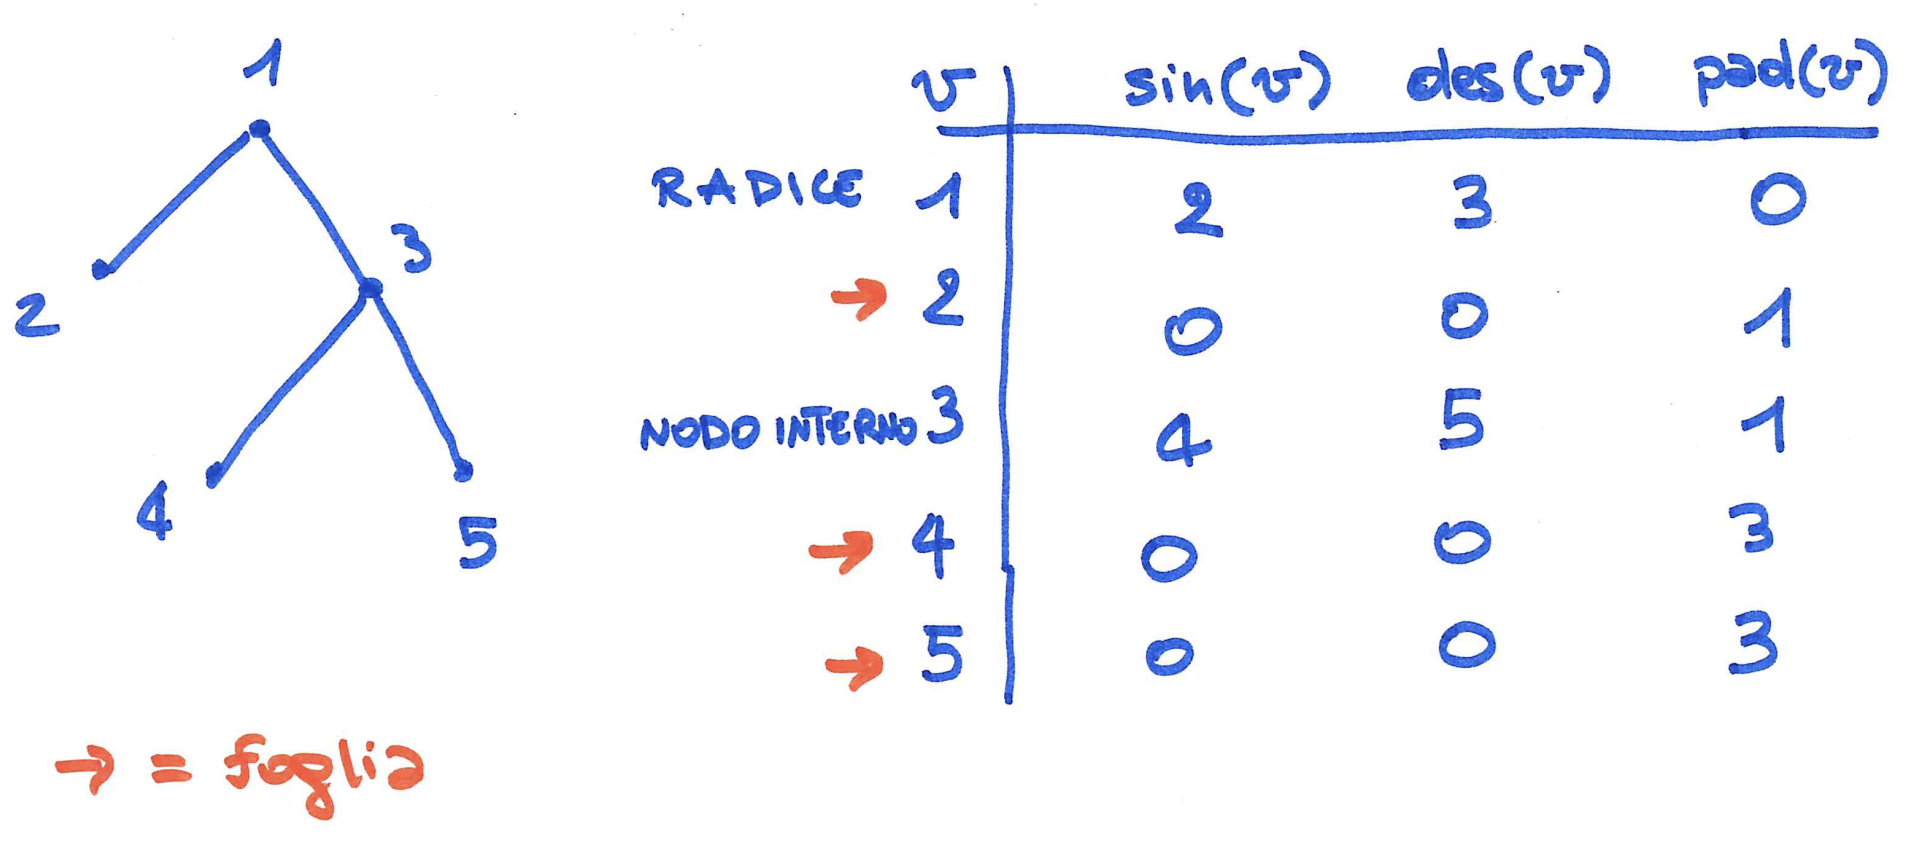
\includegraphics[scale=0.35]{images/ciclo_eureliano.png}
\end{figure}

Come posso rappresentare un albero in una tabella?
\begin{itemize}
    \item Etichetto ogni nodo dell'albero con un numero
    \item Utilizzo una tabella in cui ogni riga è dedicata ad un nodo
    \item Le informazioni che io vado a scrivere su questo nodo (nella colonna) sono: il figlio sinistro ($sin(\upsilon)$), il figlio destro ($des(\upsilon)$) e il padre ($pad(\upsilon)$)
\end{itemize}

Ci dobbiamo immaginare questa tabella in memoria. Molti problemi ben noti usano la struttura dati ad albero: ricerca, dizionari, query. L'operazione fondamentale in questi problemi è la navigazione dell'albero, anche per la manutenzione (inserimento, modifica e cancellazione) di elementi.

Come farlo con algoritmi paralleli efficienti? Usiamo le liste che si gestiscono bene in parallelo (vedi Kogge-Stone). Le liste che non sono altro che dei puntatori ai nodi dell'albero. Dobbiamo sostanzialmente definire un vettore $\vec{s}$ dei successori dell'albero. E' un vettore che lega gli elementi in un array e indica chi è il successore per ogni elemento.

\begin{enumerate}
    \item Dall'albero binario al ciclo Euleriano.\\
    Associo all'albero binario un ciclo Eureliano. Sostituisco ogni ramo dell'albero con due archi, uno che scende e uno che sale.

    \begin{figure}[h]
        \centering
        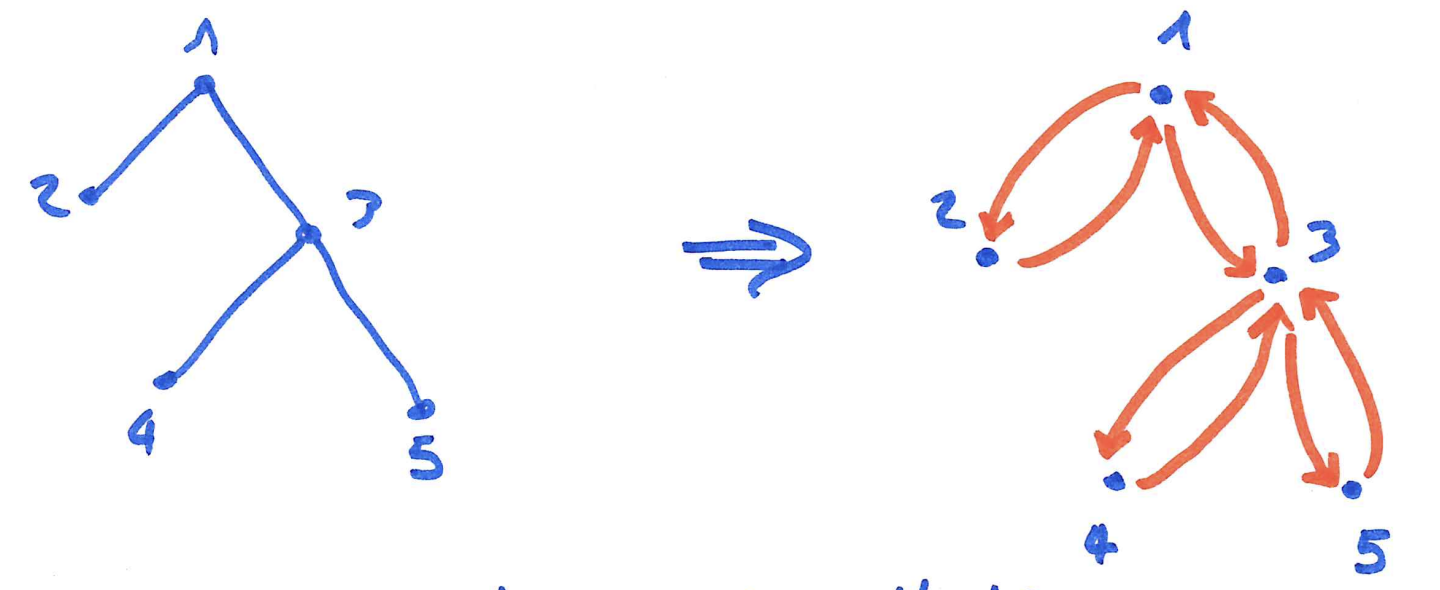
\includegraphics[scale=0.35]{images/ciclo_euleriano1.png}
        \caption{Ciclo euleriano: primo passo}
        \label{fig:my_label}
    \end{figure}

    \item Dal ciclo Eureliano al cammino Eureliano.\\
    Siccome in qualche nodo ci potrebbe essere ambiguità (potrei scendere o anche risalire), trasformo questo grafo in un altro grafo in modo da definire un cammino Eureliano, seguendo questa regola: ogni nodo $\upsilon$ viene espanso in $3$ nodi $(\upsilon, s), (\upsilon, c), (\upsilon, d)$. Rispettivamente sinistra, centro, destra.\footnote{Nonostante sia definita un'etichetta questi non sono da considerarsi degli archi ma sono da considerare come nodi}

    \begin{figure}[h]
        \centering
        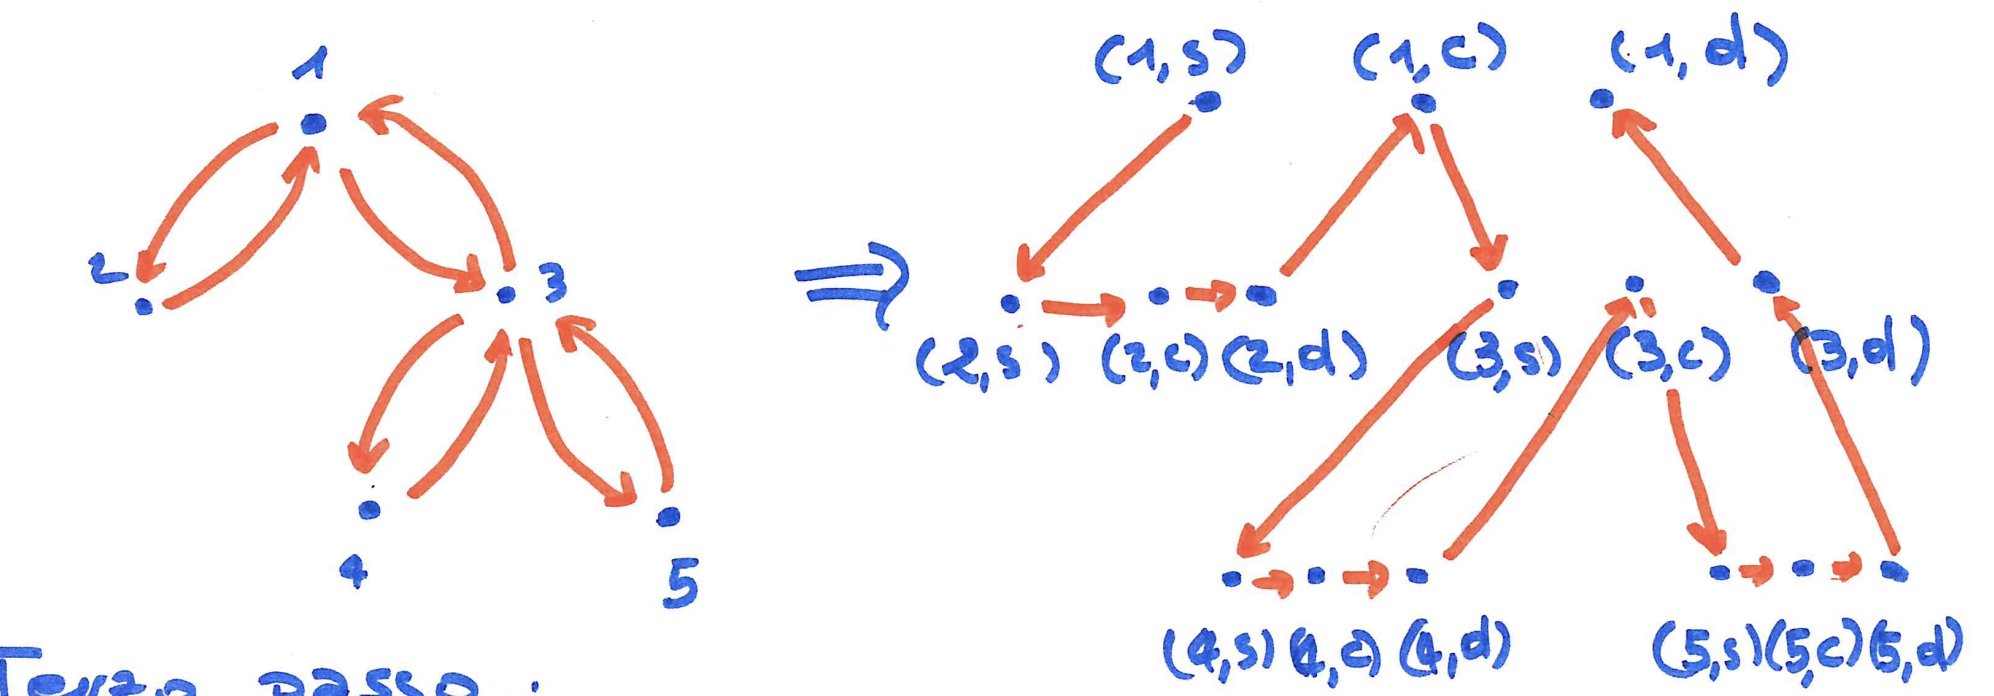
\includegraphics[scale=0.35]{images/cliclo_eureliano2.png}
        \caption{Dal ciclo al cammino Eureliano}
        \label{fig:my_label}
    \end{figure}

    Inserisco delle freccie che collegano tutti i nodi (anche quelli espansi), il cammino che esce fuori è un cammino Eureliano. Questo perchè percorro gli archi una ed una sola volta.

    \item Dal cammino Eureliano alla costruzione della lista.\\
    \uline{Sarà un vettore indicizzato dai nodi del grafo}

    $$S( (\upsilon, x) )\; dove\; 1\leq \upsilon \leq n \; , x \in \{s,c,d\} $$

    \item Costruzione dell'array\\
    Abbiamo delle regole diverse in base a se il nodo è un nodo foglia o un nodo interno 

    Se il nodo foglia è figlio sinistro punta al centro, se figlio di destra punta al nodo padre con etichetta destra

    Se il nodo è interno, se ha un'etichetta sinistra scende al figlio di sinistra con etichetta $s$, se centro scende al figlio di destra con etichetta $s$. Quando è destro vale la stessa regola per il nodo foglia destro

    Diamo un algoritmo parallelo per costruire S. \uline{Trasforma il grafo in una lista dicendo per ogni nodo chi è il successore}. Si può pensare che la tabella è in memoria ed ogni processore prende in carico una riga della tabella (quindi di un vertice) e per ogni riga della tabella costruisce il successore

    Si può eliminare la concorrenza delle letture.
\end{enumerate}

\paragraph{Valutazione}
    Questo algoritmo (con alcuni accorgimenti per eliminare la concorrenza delle letture) risulta essere un EREW 

\paragraph{Processori}  Prima $P = n$; Dopo Willye $P = \frac{n}{\log n}$

\paragraph{Tempo} $T(n, p(n)) = O(1)$\\
Numero di processori $n$, tempo costante è uno di quei casi che ci ricorda che se raggruppiamo con $\log n$ i nostri nodi $\upsilon$ possiamo passare da $n$ a $\log n$ processori e il tempo da costante diventa logaritmico $T = \log n$

\newpage

\section{Caso parallelo a memoria distribuita}
Queste architetture possono essere visualizzate come un grafo in cui i nodi sono processori e gli archi del grafo rappresentano le connessioni dirette.

\uline{Sono processori che non condividono una memoria ma una rete di inter-connessione}, collegati da dei \uline{link full-duplex}\footnote{La comunicazione è simmetrica, può avvenire da entrambi i lati} e possono comunicare tra di loro attraverso questi. 

\paragraph{Proprietà}
In questa architettura i processori sono sincroni ma non hanno una memoria condivisa, c'è una rete di inter-connessione che li lega. In genere, una rete di inter-connessione non mi da un grafo completo. Un grafo dove i nodi sono i processori e gli archi sono i collegamenti diretti tra i processori. I processori hanno una memoria privata per poter lavorare ma manca la memoria centrale condivisa. \uline{Questi processori però condividono un unico clock centrale}. E' un modello di calcolo che da un'astrazione di com'è fatto un super-computer. \uline{Da non confondere con le architetture distribuite, dove non c'è un unico clock centrale e la rete di inter-connessione è Internet}.

Si chiamano distribuiti proprio perchè manca la memoria condivisa.

\paragraph{Caratteristiche dei processori}
Sono sempre delle RAM sequenziali. Sono elementi di calcolo e anche router perchè possono spedire e ricevere informazioni all'interno della rete, \uline{eseguono istruzioni per il calcolo con la loro memoria privata ma devono anche spedire informazioni}. Questo avviene tramite due istruzioni per la comunicazione: \textit{send, receive}.

\paragraph{Proprietà sulla comunicazione} La comunicazione avviene attraverso la spedizione in questa rete, tramite dei messaggi. Rispetto al caso delle P-RAM la comunicazione non è più costante ma dipende dalla distanza tra i processori. La comunicazione è diretta nel momento in cui tra i due processori c'è un link. Tra due processori collegati direttamente il tempo è costante e costa $2$ passi

\paragraph{Cambia Input/Output} 
Manca la memoria condivisa perciò:
\begin{itemize}
    \item Input distribuita tra i processi. Ogni processore avrà qualche dato dell'input
    \item Output o abbiamo un processore dedicato\footnote{Ad esempio il processore con indice più alto ha il risultato} o si legge in un certo ordine tra i vari processori rispettando l'indice dei processori.
\end{itemize}

\paragraph{Risorse di calcolo} Sono sempre tempo e hardware, ma il tempo oltre a contare le operazioni elementari aritmetiche e logiche, conta anche le operazioni di scambio di informazioni (è legato alla rete di connesione e può essere rilevante).

\paragraph{Parametri di rete}
Data un architettura $G=(V,E)$ si definiscono i parametri
\begin{itemize}
    \item GRADO\\
    $$\gamma = max\;\{\;\rho(\upsilon) \;|\; \upsilon \in V \}$$
    \uline{Massimo numero di archi incidenti su un nodo}. Più il grado è alto più ci sono archi, più la connessione può essere buona. Ma se alziamo troppo $\gamma$ per avere migliore comunicazione più difficile diventa la realizzazione fisica
    \item DIAMETRO\\
    $$\delta = max\;\{\;d(\upsilon, \omega)\;|\;\upsilon \neq \omega \in V\;\}$$
    Per ogni coppia di vertici viene definita la distanza tra questi come la minima distanza per raggiungere il nodo destinazione partendo dal nodo iniziale. Questa è rappresentata da $d(\upsilon, \omega)$. \uline{Il diametro è la massima distanza tra due nodi nel grafo}. Valori bassi di $\delta$ sono da preferire nei nostri algoritmi, valori di $\delta$ troppo bassi aumentano il valore di $\gamma$, quindi aumentano la difficoltà della realizzazione fisica 
    \item AMPIEZZA DI BISEZIONE\\
    Si definisce come $\beta$ \uline{il minimo numero di archi in G che tolti mi dividono i nodi in circa due metà}.
    \uline{Rappresenta la capacità di trasferire le informazioni in G} da una parte all'altra del grafo, ancora una volta $\beta$ alto preferibile ma incrementa $\gamma$
\end{itemize}

\subsection{Sorting network}
In questo caso è semplice descrivere gli algoritmi come circuiti, la cui componente elementare è l’elemento \textit{confronto-scambio}, che riceve in ingresso la coppia di interi $(x,y)$ e dà in uscita la coppia, ordinata in modo crescente, $(min(x,y), max(x,y))$

Una \textit{rete di ordinamento} di $n$ interi può essere graficamente rappresentata da $n$ linee orizzontali, aventi in ingresso gli $n$ interi; ogni operazione di confronto-scambio è rappresentata da una connessione verticale tra due di queste linee

\begin{figure}[h]
    \centering
    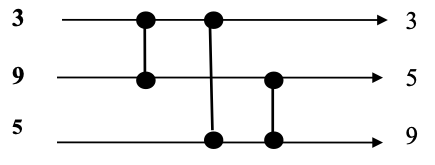
\includegraphics[scale=0.4]{images/sorting_network.png}
    \caption{Rete per l’ordinamento di $3$ interi}
\end{figure}

\begin{definizione}
    Le istruzioni di confronto per i confrontatori o comparatori
    $$\text{if}\;A[i]<A[j]\;\text{then SWAP}\;(A[i], A[j])$$
    $$\text{if}\;A[i]>A[j]\;\text{then SWAP}\;(A[i], A[j])$$
\end{definizione}

Insieme di confrontatori tali per cui passandogli un input mi torna un output ordinato. Formalmente definiamo una rete di confrontatori con
$$R(x_1, \dots , x_n) = (y_1, \dots , y_n)$$
Si dice che R è una sorting network sse 
$$\forall (x_1, \dots , x_n) \in N^2 \; vale\; R \; con\; y_1 < y_2 < \dots < y_n$$

Queste reti si chiamano anche reti di ordinamento \textit{TEST/SWAP OBLIVIOUS}, deriva dal fatto che i confronti che vengono eseguiti non dipendono dall'input, sono state fissate a priori, vengono effettuati qualunque sia l'input. Come faccio a sapere se R è una sorting network?

\paragraph{Principio 0-1 (Knut 1972)}
Uno strumento che grandemente semplifica le dimostrazioni di correttezza delle procedure di ordinamento su reti. Valuto la sorting network solo su valori binari

\begin{definizione}
    Se una rete di ordinamento R lavora correttamente su vettori con componenti in ${0,1}$, allora lavora correttamente per qualsiasi vettore di interi
\end{definizione}

\paragraph{Asserzione di Knut}
$$\exists \; x \in N^n \;t.c\; R(x)\;non\;e'\;ordinato$$
Esiste un $x$ che non viene ordinato da $R$.
$$\exists \; x \in \{0,1\}^n \;t.c\; R(x)\;non\;e'\;ordinato$$
Cioè non funziona bene nemmeno in binario

\paragraph{Dimostrazione Knut}
All'input prima viene applicata la funzione \textit{f}, in uscita viene applicata \textit{R} che è la mia rete di confrontatori. Il risultato non cambia se shiftiamo f su R, cioè se invertiamo (prima R poi f). \uline{Affinchè questo sia vero bisogna assumere che la funzione \textit{f} sia monotona crescente}. \uline{f-shift su R vale per ogni f monotona crescente}

Se esiste un $x$ tale che $R(x)$ non lo ordina deve valere che $R(x)$ restituisce un vettore $y$ dato dalle componenti $y_1, \dots, y_n$ tale che due elementi non sono ordinati. Deve esistere un $y_k$ che precede un $y_s$ che è più grande.

$$\exists\; x \in N^n \;t.c.\; R(x) = (y_1, \dots, y_k, y_s, \dots, y_n )\; con\; y_k > y_s$$

Definiamo una funzione G monotona crescente $N \rightarrow {0,1}$
\begin{equation}
    g(x) = 
        \begin{cases}
            1 & \text{se $x \geq y_k$}\\
            0 & \text{altrimenti}
        \end{cases}
\end{equation}

Calcolo R su un vettore binario 
$$R(g(x_1), \dots , g(x_n))$$
Posso applicare la regola dello shift (g-shift), prima applico R poi g, otteniamo in ouput un vettore binario e dobbiamo vedere se è stato ordinato oppure no
$$= (g(x_1), \dots , g(y_k), \dots, g(y_s), \dots , g(y_n))$$

Non è ordinato perchè $y_k > y_s$. La rete sbagliava su $x$, sbaglia anche sul binario.

\begin{osservazione}
Come faccio a sapere se R è una sorting network? Se voglio scoprire se una rete è una sorting network mi basta valutare R solo su input binari.
\end{osservazione}

\subsection{Array lineare}
Sono un'architettura a memoria distribuita. I processori sono connessi uno in fila all'altro su una riga. Ogni processore è collegato al processore precedente e al suo successivo

\paragraph{Parametri di rete}
$\gamma = 2\;, \;\delta = n-1\; ,\; \beta = 1$. Un $\gamma$ così è il più basso che possiamo avere, altrimenti non ci sarebbero i collegamenti. $\delta$ rappresenta la distanza tra i processori più ”lontani” $P_1$ e $P_n$

Nelle P-RAM il tempo è esattamente il tempo dei conti, mentre in questo caso c'è anche il tempo di comunicazione, che non è costante, perciò non sarà possibile ottenere tempi logaritmici.

\subsubsection{Shuffle}
Prende un array lo divide a metà e intercala la prima metà con la seconda metà facendo in prima posizione il primo elemento della prima metà, in seconda posizione il primo elemento della seconda metà poi di nuovo il primo elemento etc$\dots$.   \uline{Mischia intercalando uno della prima metà con uno della seconda metà}

\paragraph{Primitiva shuffle}
Servirà anche sull'ordinamento per altre architetture parallele come Mesh, \uline{swap contiguo}

$$SWAP (k, k+1)$$

Abbiamo due processori consecutivi $P_k$ e $P_{k+1}$ collegati direttamente perchè consecutivi. Il primo ha il dato $A[k]$, il secondo $A[k+1]$. Si richiede di swappare i contenuti. Si utilizzano le istruzioni \uline{send} e \uline{receive}.

In un passo (un giro di clock) fanno le send, all'istante dopo fanno due receive per leggere il dato che gli è stato spedito. \uline{Il numero di passi per questa primitiva è costante ($3$ passi)}. E' costante perchè i processori sono collegati tra di loro

\paragraph{Shuffle}.\\
Input: $A[1]\;A[2]\dots A[s]\;A[s+1]\dots A[2s]$\\
Output: $A[1]\;A[s+1]\;A[2]\;A[s+2]\dots A[s]\;A[2s]$

\uline{In input abbiamo un vettore di lunghezza pari}, in output desideriamo una prima metà dell'input innestata dalla seconda metà. Ossia, vogliamo in output che le due metà siano mischiate.

Sostanzialmente alterniamo i nostri elementi in questo modo: un elemento della prima metà, un elemento della seconda metà.

Su un array lineare di n elementi, lo SHUFFLE di $(a[1], a[2], a[3], \dots, a[2s])$ può essere ottenuto in tempo $O(s)$ da un procedura SHUFFLE con scambi a “triangolo”

\begin{figure}[h]
    \centering
    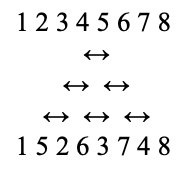
\includegraphics[scale=0.40]{images/shuffle.png}
\end{figure}

\paragraph{Numero di processori}
processori = $2(s-1)$ perchè il primo e l'ultimo elemento non vengono mai scambiati, perciò si può evitare di assegnare un processore

\paragraph{Tempo}
Numero di passi $3$. Tempo parallelo $3(s-1)$, si conta la diagonale sul grafico e risultano essere la metà del nostro input

\paragraph{Efficienza}
Sopra c'è il costo dello shuffle sequenziale senza supporre di avere una memoria aggiuntiva. Sotto numero di processori per tempo parallelo. Il risultato è un algoritmo ottimale.
$$E \approx \frac{s^2}{s\;*\;s} = C$$

\subsubsection{Max}
Visto che i dati sono distribuiti nelle memorie private dei nostri processori ci sarà la richiesta di spedizione del dato. $P_i$ deve spedire il proprio dato $A[i]$ al processore $j$.

\paragraph{Primitiva Max}
$SEND(i,j)$ dove $i$ è il sender, $j$ il receiver. Entra in gioco la distanza tra i due processori


\paragraph{Max}.\\
Input: $A[1]\;A[2]\dots A[n]$\\
Ouput: $contenuto(P_n) = max\{\;A[i]\;|\;1 \leq i \leq n\;\}$

\uline{Mettiamo il risultato nel processore che ha indice più alto}. Il tempo per MAX su array lineari è limitato inferiormente da \textit{n}. Anche qui possiamo applicare l'idea di Wyllie

\begin{enumerate}
    \item Si considera l'algoritmo per SOMMATORIA delle P-RAM
    \item Riduzione dei processori per abbassare $\Omega(n)$ su array ad $n$ processori, che può essere confrontato con il tempo degli algoritmi sequenziali per risolvere lo stesso problema
\end{enumerate}

Stesso ragionamento che si fa per sommatoria, al j-esimo passo si confrontano i numeri a distanza $2^{j-1}$

\begin{itemize}
    \item Confronto con numeri a distanza $2^j-1$
    \item Selezione del max
    \item Memorizzo nel processore di indice $2^j\;*\;t$
\end{itemize}

\paragraph{Codice}
\begin{minted}
[
frame=lines,
framesep=2mm,
baselinestretch=1.2,
bgcolor=white,
fontsize=\footnotesize,
linenos
]{python}
for j in range(1, logn + 1):
    for t in range(1, n // (2**j) + 1):
        k = 2**j * t - 2**(j-1)
        SEND(k, k + 2**(j-1))

    for t in range(1, n // (n // (2**j)) + 1):
        k = 2**j * t
        if A[k] < A[k - 2**(j-1)]:
            A[k] = A[k - 2**(j-1)]
\end{minted}

\paragraph{Tempo}
Calcoliamo il tempo per la \textit{send} e il tempo per il \textit{compare} poi moltiplichiamo per $\log n$. La prima è $2$ volte la distanza tra i processori quindi $2*2^{j-1}$. La seconda fase richiede un confronto ed un eventuale assegnamento, quindi costa $2$

$$Totale = \sum_{j=1}^{\log n} 2\; 2^{j-1} + \sum_{j=1}^{\log n} 2 = \sum_{j=1}^{\log n} 2^j + 2\log n = 2^{\log n+1}-1-1 + 2 \log n = 2n - 2 + 2 \log n = O(n)$$

\paragraph{Processori} Il numero dei processori è tanto quanto la lunghezza dell'input $n$

\paragraph{Efficienza} $E \rightarrow 0$, non va bene

\paragraph{Nuovo algoritmo}
\begin{osservazione}
    Se riduciamo i processori da $n$ a $p$, ogni processore deve prendersi $\frac{n}{p}$ elementi. In questo modo operiamo sul parametro $\delta$ cioè la distanza massima tra i processori, perchè da $n$ sono passato ad un array di $p$ elementi e questo valore viene ridotto
\end{osservazione}
\begin{itemize}
    \item Un processore seleziona il max sequenzialmente tra i suoi $\frac{n}{p}$ processori
    \item Si esegue il codice per MAX su $p$ processori (fase di spedizione dei massimi)
\end{itemize}

\paragraph{Prestazioni} Processori: P; Tempo parallelo: $O(\frac{n}{p}) + O(p)$

\paragraph{Efficienza}
Al numeratore abbiamo $n$ (calcolo del massimo sequenzialmente, tempo lineare) al denominatore abbiamo $P\;*\;tempo\;parallelo$ $P(O\frac{n}{p} + O(p)) = O(n) + O(p^2)$

Per avere $E \rightarrow C \neq 0$ scelgo $p^2 = n$. Scelgo $p$ in modo tale che il quadrato mi da n, cioè $p = \sqrt{n}$

Di conseguenza MAX è risolto efficientemente su array lineari con $P=\sqrt{n}$ e 
$$T=O(\frac{n}{\sqrt{n}} + O(\sqrt{n})) = O(\sqrt{n})$$


\subsubsection{Ordinamento}
In questo caso lo SWAP può essere anche su processori non contigui, \uline{generalizziamo l'operazione di SWAP}.

\paragraph{Primitiva}
MINMAX $(K, K+1)$. Abbiamo due processori $P_k$ e $P_{k+1}$, il primo deve contenere il minimo valore, il secondo deve contenere il massimo. \uline{Questo problema è del tutto simile allo SWAP, ma non sempre avviene lo scambio di dati}. \uline{Al posto di esserci l'assegnamento sicuro, c'è un assegnamento condizionato}. C'è un if e poi un eventuale assegnamento, il numero di passi paralleli per risolverlo è un passo in più, quindi $4$

\uline{Minmax è la primitiva che realizza il confrontatore nelle sorting network}

\paragraph{Ordinamento}
Abbiamo $n$ dati, ognuno viene lasciato ad un processore. Come output desideriamo leggere il risultato sui nostri processori seguendo l'indice dei processori.

\paragraph{ODD/EVEN sorting network} Un algoritmo \textit{test/swap oblivious} descritto da una sorting network

L'ordinamento odd-even è un algoritmo di ordinamento parallelo che viene utilizzato per ordinare una serie di elementi in modo efficiente su più processori o su una rete di calcolatori. \uline{L'algoritmo funziona confrontando elementi in posizioni dispari con elementi in posizioni pari e scambiandoli se sono in ordine sbagliato}. Ciò viene ripetuto per ogni coppia di elementi consecutivi nella serie, fino a quando l'intera serie non è stata ordinata

\begin{figure}[h]
    \centering
    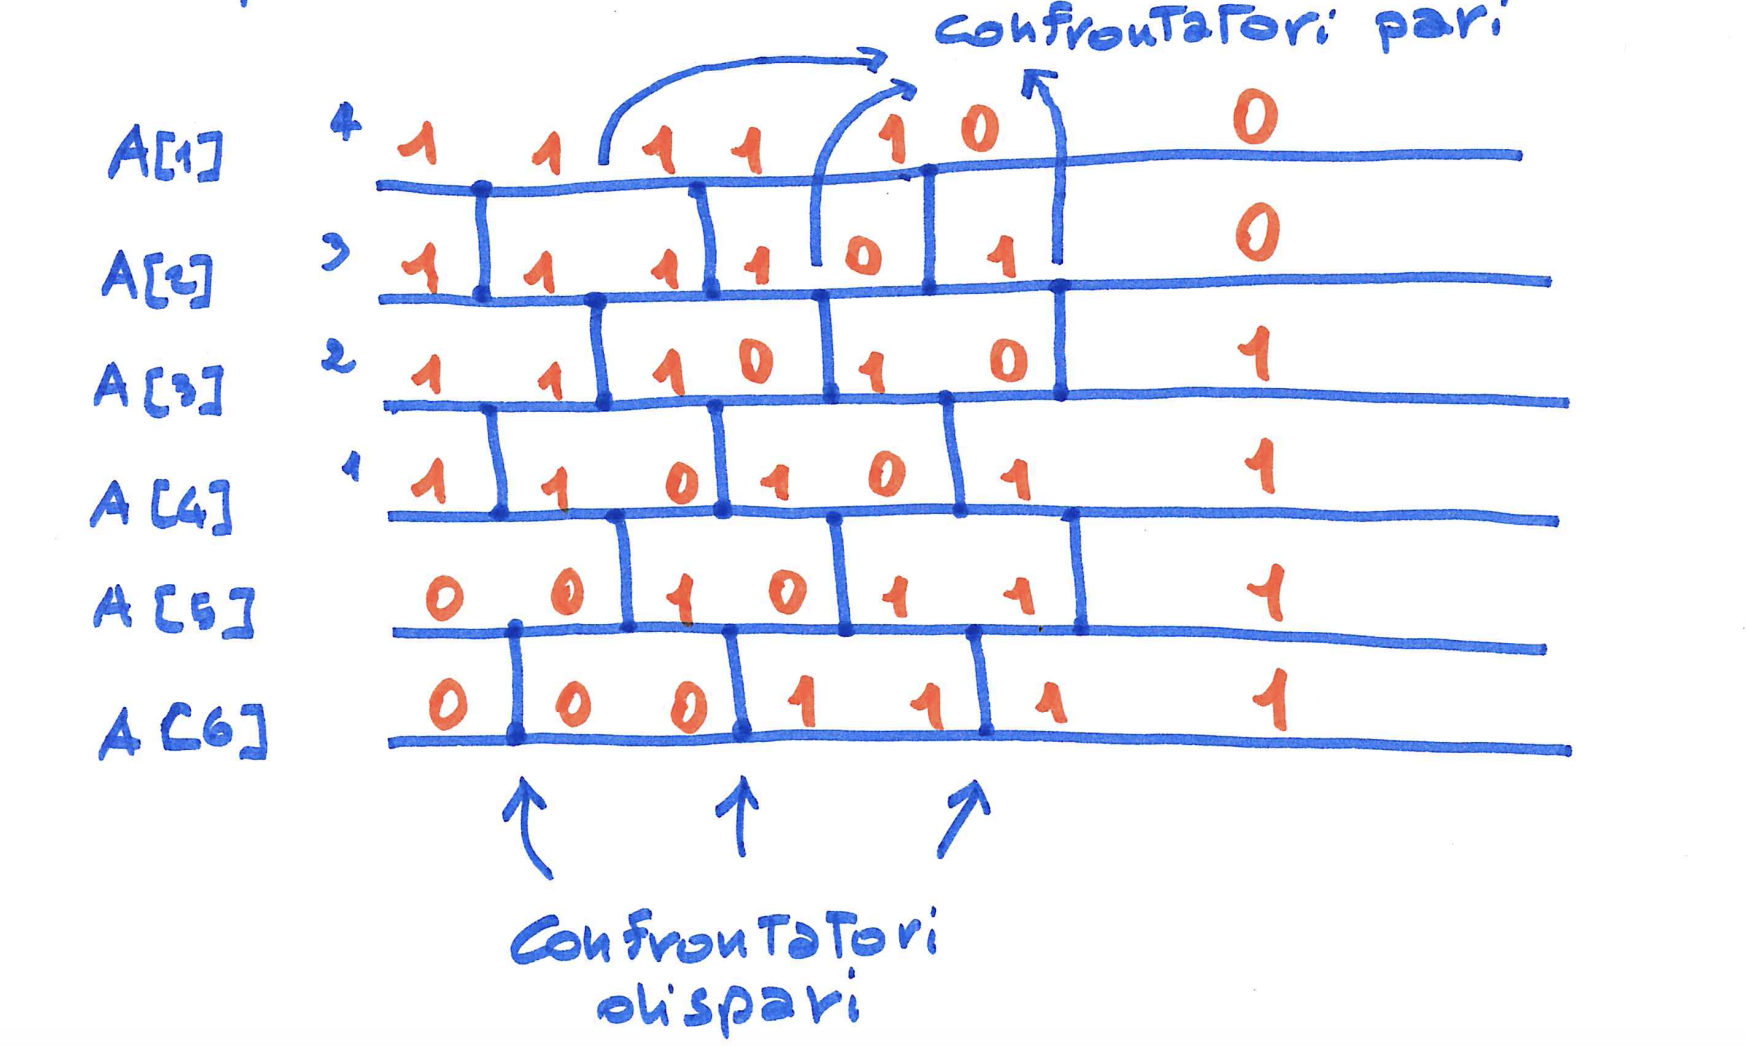
\includegraphics[scale=0.4]{images/odd_even.png}
    \caption{Esempio con 6 elementi da ordinare}
\end{figure}

Al primo passo non viene mai confrontato un $1$ con uno $0$. Il primo passo non scambia nessun elemento dell'input. Esempio: il secondo $0$ inizia a muoversi dal terzo passo

\uline{Per la correttezza di ODD/EVEN usiamo il principio $0-1$ (Knuth)}. Se questa rete mi ordina tutti i numeri binari, allora è una rete che è corretta anche sui numeri naturali. 

$$\{0,1\}^n \rightarrow\;odd/even\; \rightarrow 0^j1^e\;con\;j+e=n$$

\paragraph{Dimostrazione}
Ci vogliono $n$ round, che sono necessari si vede dall'esempio, ma che sono sufficienti lo dobbiamo dimostrare

Partiamo dall'esempio, abbiamo $4$ volte $1$ e $2$ volte $0$, quindi $e=4\;;\;j=2$

\begin{osservazione}
    Nel nostro caso ogni $1$ deve scendere di $n - e = j = \# 0$ posizioni. Cioè ogni $1$ deve scendere di almeno $2$ posizioni.
\end{osservazione}

Si possono studiare gli $1$ dal basso più il ritardo. Il massimo ritardo che si può avere è il numero di $1$ dell'input
\begin{itemize}
    \item La regola è che l'i-esimo dal basso impiega $n - e + i$ passi
    \item In generale è un \textit{al più} $n - e + i$ passi
    \item Dato che $i \leq e$ si ottiene $n - e + e = n$ passi, al più $n$ passi $\implies n$ passi di ODD/EVEN sono necessari e sufficienti
\end{itemize}

\paragraph{Implementazione con codice}
\begin{itemize}
    \item Sequenziale $T(n) = O(n^2)$
    \item Parallelo Haberman $'72$\\
    $n$ passi paralleli o round di comparatori implementati con MINMAX
    \begin{lstlisting}
        for i = 1 to n
            for k in {2t - (i%2) | 1 <= t <= n/2} par do
                MINMAX(k, k+1)
    \end{lstlisting}

    Il primo round fa lavorare con MINMAX quelli con indice dispari
\end{itemize}

\paragraph{Tempo}
For esterno mi dice quanti round ci sono, n colonne di comparatori. Il MINMAX che viene eseguito in parallelo dal for par do richiede $4$ istruzioni (come lo SWAP ma con il confronto), perciò

$$n * 4 = O(n)$$

dove $n$ è il numero di round e $4$ è il min-max in parallelo

\paragraph{Efficienza}
$$\frac{n\;\log n}{n\;n} \rightarrow 0 $$

%Riduzione dei processori
\begin{comment}
    \paragraph{Riduzione dei processori}
Primo step: ogni processore si prende $\frac{n}{p}$ dati e li ordina
\end{comment}

\paragraph{Primitiva MERGE-SPLIT}
La primitiva MERGE-SPLIT avviene tra due processori contigui
\begin{itemize}
    \item Il processore di sinistra spedisce $\frac{n}{p}$ dati ordinati al processore di destra. Questo ha tempo $O(\frac{n}{p})$
    \item (MERGE) Il processore di destra riceve e fonde i nuovi $\frac{n}{p}$ con i suoi $\frac{n}{p}$ dati (ordinati). Questo ha tempo $O(\frac{n}{p})$
    \item (SPLIT) Il processore di destra invia i dati più piccoli $\frac{n}{p}$ al processore di sinistra
\end{itemize}

Come il codice precedente ma al posto di MINMAX c'è il MERGESPLIT. \uline{E' ODD-EVEN dove minmax è sostituito con la primitiva merge-split}. \uline{Ogni singola primitiva merge-split viene ripetuta per P round}

\paragraph{Tempo}
$$\frac{n}{p} \log \frac{n}{p} + p * \frac{n}{p} = O(n)$$
Primo passo che è sequenziale e lo fanno tutti i processori, più p round per merge-split che richiede $\frac{n}{p}$, le $p$ si semplificano

\paragraph{Denominatore di E}
TODO $\dots$

\paragraph{Efficienza}
$$\frac{n \log n}{n \log n} \rightarrow C \neq 0$$

\begin{osservazione}
    Il tempo è rimasto $O(n)$, ciò si spiega in quanto la riduzione dei processori agisce sul diametro e non sull'ampiezza di bisezione, $\beta = 1$
\end{osservazione}


%Mesh
\subsection{Architetture Mesh}
Processori strutturati a forma di quadrato, con delle connessioni sia per riga che per colonna. Un quadrato di processori connessi sia per riga che per colonna. \uline{Array bi-dimensionale, ovvero una griglia di processori}. I processori sono messi in un quadrato di lato $\sqrt{n}$

\begin{figure}[h]
    \centering
    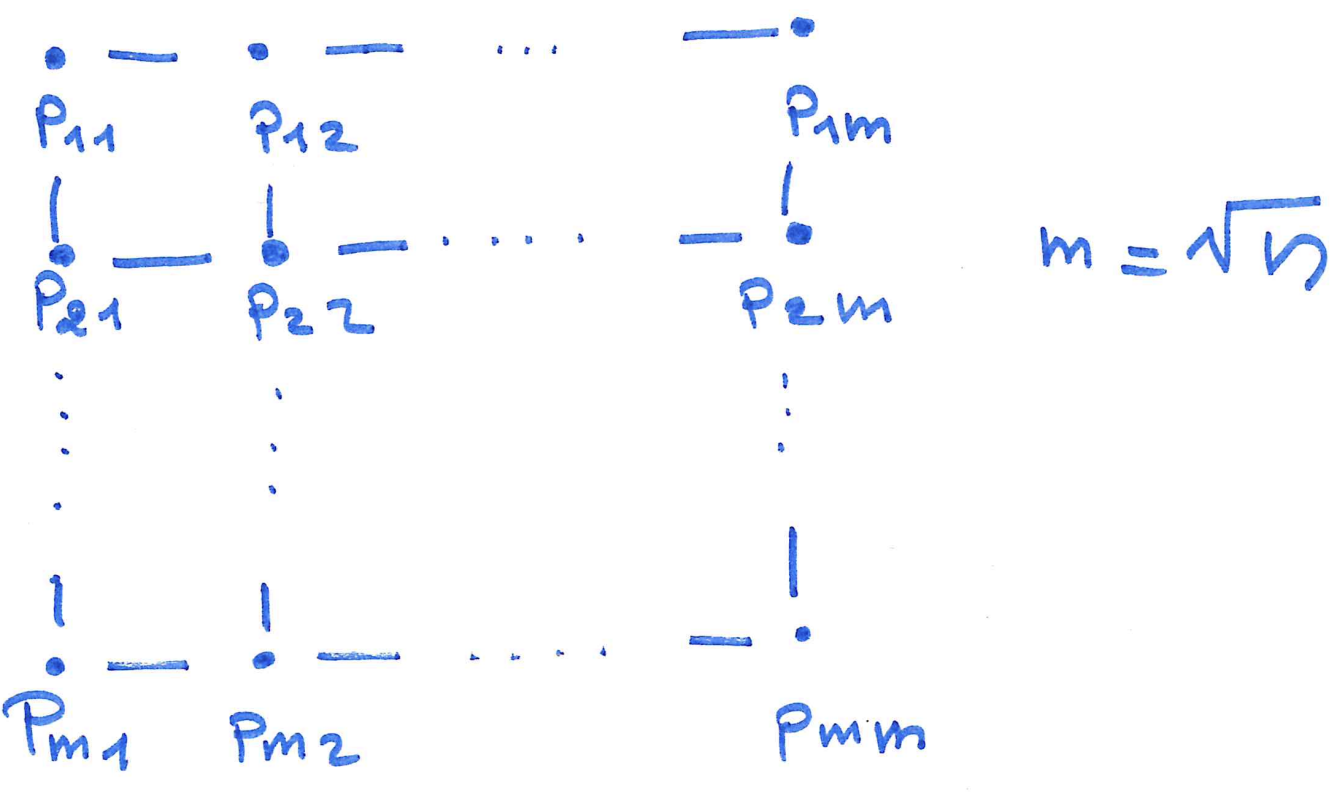
\includegraphics[scale=0.4]{images/architetture_mesh.png}
\end{figure}

\paragraph{Parametri di rete}
\begin{itemize}
    \item $\gamma = 4$ (grado). Il massimo numero di archi incidenti su un nodo, due rivolti sulla riga, due sulle colonne
    \item $\delta = 2\sqrt{n-1}$ (diametro), perchè ci sono i link verticali ed orizzontali quindi percorro la diagonale. I processori più “lontani” sono $P_{11}$ e $P_{mm}$ : essi sono collegati da un cammino di $2(m-1)$ passi.
    \item $\beta \approx \sqrt{n} $, posso tagliare a metà della prima colonna con una riga orizzontale oppure in verticale
\end{itemize}

\begin{figure}[h]
    \centering
    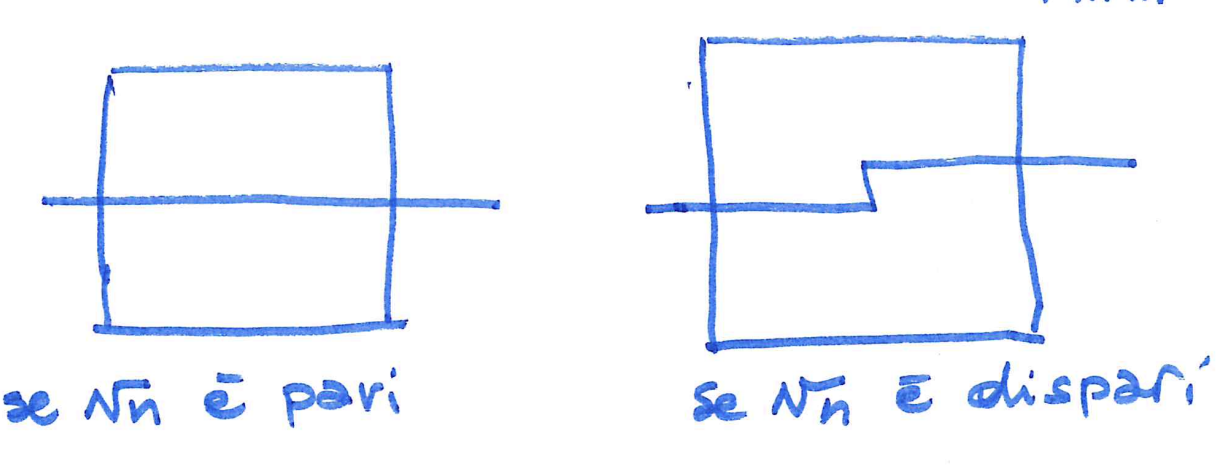
\includegraphics[scale=0.4]{images/architettura_mesh2.png}
\end{figure}

\paragraph{Lower bound}
Visto che il diametro e il $\beta$ sono nell'ordine $\sqrt{n}$ abbiamo questi lower bound
\begin{itemize}
    \item MAX $\Omega(\sqrt{n})$
    \item ORDINAMENTO $\Omega(\sqrt{n})$
\end{itemize}

\subsubsection{Max}
\paragraph{Serpente}
Potremmo vedere nella nostra architettura mesh un "serpente" di processori. Posso costruire un percorso a serpente fino ad arrivare all'ultima riga, ottenendo così un array lineare. A questo punto prendo l'algoritmo del massimo su array lineare e lo eseguo

\uline{Usiamo la Mesh come array lineare}. In questo serpente ci sono $n$ processori e la distanza tra due processori più lontani risulta essere $n$ e quindi la soluzione sul serpente non può richiedere meno di $n$ passi paralleli, e non va bene visto il lower bound.

Definisce un ordine con cui leggere i dati nella mesh, i primi $m$ valori vengono dati sulla prima riga, nella seconda riga si va da destra verso sinistra. Anche l'output dovrà essere letto in questo modo

Se vogliamo sfruttare questo come un array lineare non otteniamo dei risultati migliori dell'array lineare 

\paragraph{Algoritmo RIGHE-COLONNA per MAX}
\uline{Ogni riga dell'array e l'ultima colonna sono viste come array lineare di $\sqrt{n}$ processori separati}. Posso calcolare il massimo su ogni riga, sposto l'elemento massimo di ogni riga nell'ultima posizione della riga. Dopodichè nell'ultima colonna ho tutti gli elementi massimi e posso calcolare il massimo degli elementi massimi vedendo questa colonna come un array lineare che verrà posizionato in $P_{mm}$.

\paragraph{Codice}
\begin{minted}
[
frame=lines,
framesep=2mm,
baselinestretch=1.2,
bgcolor=white,
fontsize=\footnotesize,
linenos
]{python}
for i in range(1, int(sqrt(n)) + 1):
    MAX(pi, pi2, ..., pim)
    +
    MAX(p1m, p2m, ..., pmm)
\end{minted}
Il primo MAX fa il massimo di un'array lineare di ogni riga $i$ che va da $1$ a $\sqrt{n}$. Richiede come tempo/numero di passi pari alla dimensione dell'array lineare ($\sqrt{n}$)

Il secondo MAX è il massimo dell'ultima colonna. Entrambi i max hanno tempo $\sqrt{n}$, quindi $O(\sqrt{n})$, come il lower bound. I processori coinvolti sono quelli con indice pari ad $m$, anche questi formano un array lineare, l'ultima colonna.

\paragraph{Efficienza}
$$E = \frac{n}{n\;\sqrt{n}} \rightarrow 0$$
La cosa non funziona bene, l'idea è quella di operare una \uline{riduzione dei processori} per ottenere un'efficienza migliore

\paragraph{Operiamo una riduzione dei processori}
Il numero dei processori va da $n$ a $p$. Ogni processore si prenderà un gruppetto $\frac{n}{p}$ elementi su cui calcolare il massimo

\begin{itemize}
    \item Ogni processore calcola il MAX tra $\frac{n}{p}$ dati che richiede un tempo sequenziale di $O(\frac{n}{p})$
    \item Si attiva l'algoritmo RIGHE-COLONNE però su una griglia che non è più $\sqrt{n}\;*\;\sqrt{n}$ ma è diventata $\sqrt{p}\;*\;\sqrt{p}$. La nostra gliglia ha lato $\sqrt{p}$, quindi il tempo è $O(\sqrt{p})$, sommando la prima fase $O(\sqrt{p}) + \frac{n}{p} + \sqrt{p}$
\end{itemize}

Voglio un'efficienza che sia $\frac{n}{n}$, perciò scelgio $p^{\frac{3}{2}} = n \implies p = \sqrt[3]{n^2} = n^{\frac{2}{3}}$

\paragraph{Tempo}
Prima fase costa $\sqrt[3]{n}$, seconda fase $\sqrt[3]{n}$, in totale avrò $O(\sqrt[3]{n})$

\subsubsection{Ordinamento}
\textbf{Input}: $n$ numeri distribuiti uno per processore. Se l'indice della riga è dispari vengono distribuiti da sinistra verso destra, se pari da destra verso sinistra (a serpente)\\
\textbf{Output}: $n$ numeri ordinati secondo il percorso a \textit{serpente}. Ci aspettiamo un output ordinato crescente

Presentiamo qui un algoritmo che risolve su mesh il problema ORDINAMENTO in tempo ottimo $O(n)$; \uline{per semplicità, prenderemo in considerazione mesh $mxm$ dove m è potenza di $2$}

\paragraph{Ordinamento LS3}
Il nome deriva dai cognomi degli inventori degli anni $'80$. L'algoritmo è \uline{ricorsivo}, cioè richiama se stesso su istanze più piccole, applicando la tecnica \uline{dividi-et-impera}.

Chiamiamo $M$ l'intero quadrato dei processori

Esattamente come il \textit{Merge-sort}, ma quest'ultimo non prendeva i dati dalla struttura di un quadrato ma da una riga.

\paragraph{Dividi}
Abbiamo una struttura quadrata, va rispettata questa forma e si divide il quadrato in $4$ sotto-quadrati di lato la metà. Se il lato è $n$, dividiamo l'input in quadrati di dimensione $\frac{n}{2}$


\paragraph{Ordina}
Con le chiamate ricorsive si riesce ad ordinare ogni metà. Leggiamo l'input ordinato a \textit{serpente}


\paragraph{Fondi}
Una volta che arrivano quattro matrici ordinate $M_1, M_2, M_3, M_4$ l'algoritmo fonde restituendo la matrice M totalmente ordinata. Gli elementi si leggono a \textit{serpente}

\paragraph{Codice parallelo}.
\begin{minted}
[
frame=lines,
framesep=2mm,
baselinestretch=1.2,
bgcolor=white,
fontsize=\footnotesize,
linenos
]{python}
procedure LS3sort(M):
    if len(M) == 1:
        return M
    else:
        M1 = LS3sort(M1)
        M2 = LS3sort(M2)
        M3 = LS3sort(M3)
        M4 = LS3sort(M4)
        return LS3merge(M1, M2, M3, M4)
\end{minted}

Le chiamate \textit{LS3sort} sono in parallelo

\paragraph{LS3merge}
Si fanno due operazioni
\begin{itemize}
    \item SHUFFLE\\
    In LS3merge si fa shuffle di ogni riga. \uline{Prende tutte le matrici e la considera un'unica matrice}, facendo shuffle sulle sue righe. Alternando un elemento della prima metà con un elemento della seconda metà. Si costruisce M in questo modo. \uline{Inframezzare ed alternare un elemento della prima metà con un elemento della seconda metà}
    
    \item ODD/EVEN\\
    Ordinamento odd/even su due colonne adiacenti. Vuole vedere queste due colonne come un array lineare, anche questa volta le connessioni sono fatte a serpente. 
\end{itemize}

\paragraph{LS3merge: codice}.
\begin{minted}
[
frame=lines,
framesep=2mm,
baselinestretch=1.2,
bgcolor=white,
fontsize=\footnotesize,
linenos
]{python}
procedure LS3merge(M1, M2, M3, M4):
    for i in range(1, int(sqrt(n)) + 1):
        SHUFFLE(i)

    for i in range(1, int(sqrt(n/2)) + 1):
        ODD_EVEN(2*i - 1, 2*i)

    execute the first 2 * sqrt(n) steps of ODD_EVEN
    on the entire mesh (in a snake pattern)
\end{minted}

\paragraph{LS3merge: tempo parallelo}

Tutti e $3$ i passaggi del codice hanno tempo $O(\sqrt{n})$ perciò
$T_{merge}(n) = h\sqrt{n}$

\paragraph{Tempo}
Equazione di ricorrenza
\begin{equation}
    T(n) = 
        \begin{cases}
            1 & \text{se $n=1$}\\
            $T(N/4) + h\sqrt{n} & \text{altrimenti}$
        \end{cases}
\end{equation}

\newpage




\section{Ambiente di calcolo distribuito}
Abbiamo un'architettura distribuita e vogliamo risolvere i problemi legati alla comunicazione sulla nostra architettura. In particolare vedremo problemi che vogliono \uline{sincronizzare i nostri processori perchè non hanno un clock globale}

\paragraph{Rappresentazione come grafo}
Un sistema distribuito è rappresentato come un grafo dove i vertici sono le entità (processori) e tra queste entità ci sono dei link (connessioni) che permettono la comunicazione tra loro. Non è detto che le connessioni siano full-duplex ma può essere anche unidirezionale.

\paragraph{Entità}
Ogni entità possiede 
\begin{itemize}
    \item Memoria locale, all'interno di questa
    \begin{itemize}
        \item Registri di input: \textbf{valore($x$)}, intendiamo l'input dell'entità $x$
        \item Registro di stato: \textbf{stato($x$)}, quello che fa capire all'entità la situazione in cui si trova. In base al proprio stato esegue certe operazioni piuttosto che altre. \uline{E' un registro che viene modificato localmente dalla stessa entità $x$}
    \end{itemize}
    \item Capacità di calcolo
    \item Capacità di comunicazione
    \item Clock locale che scandisce il tempo, non c'è una sincronizzazione tra le entità.\uline{ E' questo l'elemento che differenzia un'architettura distribuita da una parallela}.
\end{itemize}

Esempi di entità: processori, processi, sensori, switch

\paragraph{Proprietà delle entità}
\begin{enumerate}
    \item Le entità sono reattive
    
    Solo quando accade un certo \textit{evento} compiono un \textit{azione}.\\
    Un \uline{evento} può essere \uline{interno} al sistema (ricezione di messaggi, sveglia) o \uline{esterno} al sistema (impulso spontaneo/start), è l'entità che da lo start all'algoritmo distribuito
    
    Un'azione è una sequenza finita di operazioni. Cioè come rispondono i processori agli eventi. Non è possibile bloccare l'esecuzione dell'azione
    \item Le entità seguono delle regole
    \begin{definizione}
        Una regola è un oggetto della forma $stato\;x\;evento\rightarrow\;azione$
    \end{definizione}
    \begin{definizione}
        Sia $x$ un'entità, indichiamo con $B(x)$ l'insieme delle regole a cui è soggetta $x$. $B(x)$ deve essere completo e non ambiguo, cioè ad ogni evento deve essere associata un'azione e non dobbiamo associare azioni diverse allo stesso stato-evento. $B(x)$ è anche chiamato il codice di $x$, in genere vogliamo un codice che vada bene per tutte le entità

        Se $E$ è l'insieme delle entità che cooperano tra loro, $B(E) = \cup B(x)$, questo mi da l'intero comportamento del sistema. Ed è importante che sia omogeneo:
        $$\forall x,y \in E \;si\;ha\; B(x)=B(y)$$
    \end{definizione}
    \item Registro ruolo\\
    L'idea è quella di utilizzare un registro locale aggiuntivo che differenzia quelle entità che alla stessa coppia (stato, evento) hanno azioni diverse.\\
    La regola viene modificata in $\text{stato x evento} \rightarrow \text{If ruolo(x) = a then } A_a \text{ else } A_b$
\end{enumerate}

\paragraph{Proprietà della rete}
Parliamo di come le entità vedono i link. Hanno una funzione chiamata \textit{etichettatura}, la comunicazione avviene osservando le etichette
\begin{itemize}
    \item La comunicazione avviene usando una etichettatura sui link\\
    Per l'entità $x$, l'etichettatura è denotata con $\lambda x$, dato che si trova in $\vec{G}$ si indicano con
    \begin{itemize}
        \item Nin(x): vicini di ingresso di $x$
        \item Nout(x): vicini di uscita di $x$
    \end{itemize}
    \uline{Ogni entità conosce tramite la funzione $lambda$ i nomi delle porte dei link}
\end{itemize}

\paragraph{Assiomi della rete}
\begin{itemize}
        \item Ritardo finito di comunicazione. In assenza di errori, il messaggio spedito prima o poi arriverà a destinazione
        \item Orientamento locale. Ogni entità riesce a distinguere tra i suoi vicini Nin(x) e Nout(x) grazie alla conoscenza della funzione $\lambda x$
\end{itemize}

\paragraph{Parametri di rete}.\\
Numero di entità = $n$\\
Numero di link = $m$\\
Diametro della rete = $d$, è esattamente il $\delta$ delle architetture parallele 

\paragraph{Risorse di calcolo} C'è ancora il tempo, al posto dell'hardware ci sarà il costo della comunicazione quindi il numero di messaggi che definisce la congestione del sistema nel momento in cui mandiamo in esecuzione il nostro algoritmo.

Quello che è importante è sincronizzare le risorse di calcolo, non è importante che sia veloce nel computare quanto il problema venga effettivamente risolto. \uline{C'è un'atteggiamento rivolto verso la correttezza dell'algoritmo piuttosto che sul migliorare le prestazioni}. 

\paragraph{Restrizioni sulla rete}
\begin{enumerate}
    \item Restrizioni sulla comunicazione
    \begin{itemize}
        \item Link bidirezionali, assumiamo sempre che i collegamenti tra le entità siano full-duplex
        \item Ordinamento dei messaggi\\
        I messaggi sullo stesso link vengono prelevati con la politica FIFO
    \end{itemize}
    \item Restrizioni sull'affidabilità\\
    Sono in generale delle proprietà positive della rete su cui noi facciamo affidamento, quando scriviamo il codice ad esempio dichiariamo che la rete è affidabile e non ci sono errori al momento dell'esecuzione del nostro codice. 
    \begin{itemize}
        \item Affidabilità parziale, non ci saranno errori in futuro ma ci possono essere stati in passato. Può influire sulla struttura iniziale del sistema.
        \item Affidabilità totale, non ci sono stati errori in passato e non ci saranno in futuro
    \end{itemize}
    \item Restizioni sulla topologia della rete
    \begin{itemize}
        \item Connettività del grafo\\
        Ogni entità nell'ambiente distribuito possa essere raggiunta da qualsiasi altra entità. $\vec{G}$ è fortemente connesso: per ogni coppia di entità esiste un cammino che ci faccia collegare le due entità. Cammino diretto in entrambe le direzioni                                                                                                                                                                                                                                                                                                                                                                    G è connesso, comunicazione bidirezionale
    \end{itemize}
\end{enumerate}

\begin{osservazione}
Tali restrizioni a volte vengono considerate per il calcolo delle prestazioni IDEALI del codice distribuito
\end{osservazione}

\paragraph{Misure di complessità}
\begin{enumerate}
    \item Tempo distribuito\\
    L'intervallo tra la prima entità che si attiva e l'ultima che termina. \uline{Esecuzioni diverse dello stesso codice distribuito può portare a tempi diversi}. E' un problema che si risolve osservando il TEMPO IDEALE.
    \item Numero di messaggi/quantità di comunicazione
    \begin{itemize}
        \item Numero di messaggi spediti se i messaggi sono omogenei
        \item Numero di bit spediti altrimenti
    \end{itemize}
\end{enumerate}

\paragraph{Tempo ideale} 
Tempo considerando comunicazioni unitarie (un solo giro di clock), clock sincroni.

\paragraph{Tempo causale (caso peggiore)}
Tempo misurato considerando la catena più lunga di comunicazione richiesta dal codice. E' molto più difficile calcolare questo tempo perchè bisognerebbe prendere in considerazione tutte le possibili esecuzioni, perciò il più delle volte ci si rifa al tempo ideale.

\paragraph{Definizione di un problema}
Solitamente viene definito da una tripla
$$P \;=\; <P_{init},\;P_{final},\; R>$$
Dove $P_{init}$ e $P_{final}$ sono dei predicati logici che descrivono le configurazioni del sistema all'inizio e alla fine; $R$ le restrizioni del sistema

\begin{definizione}
    Definizione di configurazione: una configurazione non è altro che una fotografia (snapshot) di un sistema in un dato tempo ed è formata da
    \begin{itemize}
        \item $E(t)$ i registri delle entità al tempo $t$ per ogni $x$ del nostro ambiente
        \item Futuro(t) gli eventi già generati al tempo $t$ ma non ancora processati
    \end{itemize}
    La coppia di questi due elementi mi da la configurazione del sistema al tempo $t$
    $$C(t) = ( E(t),\;\text{Futuro}(t) )$$
\end{definizione}

\paragraph{Algoritmo distribuito: PROTOCOLLO}
Non è proprio un algoritmo inteso come sequenza di istruzioni ma abbiamo un protocollo che è considerato un \uline{insieme di regole}, in cui il programma eseguito da un'entità risulta essere un'azione causata da un certo evento. 

stato x evento $\rightarrow$ azione\footnote{Mini-programma indivisibile, cioè operazione atomica, non si può bloccare}

Il cambiamento dello stato avviene durante l'esecuzione dell'azione. Gli eventi che azionano un'entità sono: impulso spontaneo (esterno al sistema e che starta un protocollo), sveglia o ricezione di un messaggio (interni al sistema ed eseguiti durante l'esecuzione)

Un protocollo quando viene eseguito fa cambiare configurazione al sistema. \uline{L'esecuzione di un protocollo è vista come una sequenza di configurazioni successive del sistema}

\subsection{Problemi sincronizzazione/comunicazione}
\subsubsection{Broadcasting}
Risolvere il problema del broadcast significa far si che alla fine tutte le entità abbiamo la stessa
informazione
\begin{itemize}
    \item $P_{init}$: un'entità detiene I(info). Abbiamo una entità $x$ che ha l'informazione, le altre no, hanno registro valore impostato a vuoto
    \item $P_{final}$: tutte le entità posseggono I
    $$\forall x \in E \;\text{valore}(x) = I$$
    Dove $E$ è l'ambiente distribuito, vogliamo che tutte le entità abbiano la stessa informazione
    \item $R$: link bidirezionali (BL), affidabilità totale(TR, total reliability), connettività (CN), unico inziatore (UI, unique initiator)\footnote{L'impulso spontaneo che da avvio al protocollo viene fatto su una sola entità che è quella che detiene l'informazione}
\end{itemize}

\paragraph{Stati}
Utilizzeremo due stati
$$S = \{\text{iniziatore}, \text{inattivo}\}$$
$S_{init}$ stati delle entità in $C(0)$ configurazione iniziale;\\$S_{term}$ stati delle entità in $C(f)$ configurazione finale

\paragraph{Prima versione protocollo BCAST}
.\\$S_{init} = \{\text{iniziatore}, \text{inattivo}\} = S_{start}$\\
$S_{term} = \{\text{inattivo}\}$

\begin{lstlisting}
Iniziatore:
    impulso spontaneo
    {
        send (M) to N(x)
        become inattivo;
    }

Inattivo:
    ricezione(M)
    {
        processo(M);
        send(M) to N(x);
    }
\end{lstlisting}
La forma in questo caso è stato (iniziatore/inattivo) x evento (impulso spontaneo/ricezione) esegui questa azione. $N(x)$ indica i vicini.

Il messaggio M ha la seguente forma $M = (t, o, d, I)$ dove t è la tipologia del messaggio, o e d sono origine (mittente) e destinatario, I è il campo dove c'è l'informazione che deve essere prelevata e messa nei registri valore(x).

Qual'è il problema? Il protocollo è corretto ma non termina. Viene re-inviato anche il messaggio all'iniziatore (sender) che non ne ha bisogno

La risposta al problema è stabilire più stati per le nostre entità, \uline{un raffinamento degli stati $S_{term}$}. Definiamo $S_{final} \subseteq S_{term}$ come quelli stati per cui la sola azione possibile è quella nulla. \uline{Utilizziamo un nuovo stato \textit{finito} che differisce dallo stato inattivo in cui l'unica azione possibile è quella nulla}. Grazie all'uso di questo stato il protocollo riesce a terminare.

\paragraph{Seconda versione protocollo BCAST - Flooding}
.\\$S = \{\text{iniziatore}, \text{inattivo}, \text{finito}\}$\\
$S_{init} = \text{iniziatore, inattivo} = S_{start}$\\
$S_{final} = \text{finito}$

\begin{lstlisting}
Iniziatore:
    impulso spontaneo
    {
        send(M) to n(x)
        become finito
    }

Inattivo:
    ricezione(M)
    {
        processa(M);
        send(M) to n(x)-sender;
        become finito;
    }
\end{lstlisting}

\paragraph{Flooding: complessità}
Si calcola M(numero di messaggi) e T(tempo)
\begin{itemize}
    \item $M[\text{flooding}] = \sum_{x \in E} (N(x)-1) + 1 = 2m - n + 1$
    
    Dove $m$ è il numero di archi (link) ed $n$ il numero di nodi. $2m$ perchè su ogni arco viaggiano due messaggi meno quelli del sender 
    \item $T[\text{flooding} \leq d]$

    
    Dove d è il diametro della rete. Stiamo calcolando un tempo ideale, supponendo che le entità siano sincrone e che ci sia un ritardo unitario per la ricezione dei messaggi. Il tempo ideale per Flooding è d, il diametro della rete.
\end{itemize}

\paragraph{Flooding: lower bound}
Per i lower bound si ha che
\begin{itemize}
    \item $T[\text{BCAST/RI}] \geq d$
    \item $M[\text{BCAST/RI}] \geq m$
\end{itemize}
Il protocollo flooding è ottimale

\paragraph{Flooding: dimostrazione}
Teorema: $M[\text{BCAST/RI}] \geq m$

Dimostro per assurdo, risolvo il problema con meno di $m$ messaggi. Se risolvo il problema con meno di $m$ messaggi vuol dire che sul mio grafo c'è un arco su cui non viaggiano messaggi, perchè $m$ è il numero di archi sul grafo. Il protocollo risulta corretto, ma dovrebbe funzionare su tutti i G. Costruiamo un $G\prime$ per cui A non sia corretto. Otteniamo $G\prime$ da G aggiungedo un nodo non contenuto in G. Almeno un messaggio deve passare su ogni arco, altrimenti il protocollo non è corretto.

\subsubsection{Wake Up}
Nel problema BCAST avevamo un'entità che aveva l'informazione e doveva raggiungere con un messaggio tutte le altre entità. Il problema WAKE-UP si può vedere come una generalizzazione del problema BCAST dove anzichè avere una sola entità che inizia il protocollo, ne abbiamo più di una. Rilassiamo il vincolo UI(unique initiator) e facciamo si che più entità inizialmente sono attive e inviano messaggi. 

\paragraph{Protocollo WFlood}
.\\$S = \{\text{dormiente}, \text{attivo}\}$\\
$S_{init} = \{\text{dormiente}\} = S_{start}$\\
$S_{term} = \text{attivo} = S_{final}$

\begin{lstlisting}
Dormiente
    Impulso spontaneo
    {
        SEND(w) to n(x)
        become attivo
    }

    Ricezione(w)
    {
        SEND(w) to n(x)-sender
        become attivo
    }
\end{lstlisting}

Lo stato \textit{attivo} fa le veci dello stato \textit{finito} del BCAST

\paragraph{Costo}
Visto che è una generalizzazione del BCAST, possiamo considerare il tempo ideale identico a quello visto
\begin{itemize}
    \item $T[\text{WFlood}]\leq d$
    \item $2m - n + 1 \leq M[\text{WFlood}] \leq 2m$

    
    Dove $2m$ lo otteniamo se tutte le unità si svegliano con un impulso spontaneo
\end{itemize}



\subsubsection{Traversal}
Un problema che chiede ad ogni entità di essere visitata, di attivarsi sostanzialmente, attravero l'arrivo di un messaggio. Però questa visita delle entità deve avvenire sequenzialmente, cioè una alla volta. Questa è una versione ristretta di Wake-up

\paragraph{Applicazioni} Per la gestione delle risorse condivise. La risorsa è esclusiva da parte di una sola entità, per questo è utilizzata in maniera sequenziale dalle entità


\paragraph{Configurazioni}.\\
Configurazione iniziale: tutte unvisited meno una\\
Configurazione finale: tutte visited ma una alla volta

\paragraph{Protocollo Depth-first traversal}
Visita in profondità del grafo. \uline{Si scende sempre verso il vicino non ancora visitato}

Cosa facciamo quando scendiamo e visitiamo un nodo? Inviamo un messaggio che sveglia l'entità. Usiamo un messaggio particolare TOKEN T. Quando un nodo riceve T diventa visitato ma \uline{ad ogni istante di tempo viaggia al più un solo T}

\begin{enumerate}
    \item Un nodo che riceve T per la prima volta
    \begin{itemize}
        \item Ricorda il sender
        \item Fa una lista dei suoi vicini non visitati
        \item Invia T ad uno di essi
        \item Una volta inviato il token si mette in attesa. Aspetta un messaggio di ritorno da quest'ultima entità: RETURN o BACK-EDGE

        Return quando l'entità è stata svegliata per la prima volta dal token che gli è stato inviato invece \textit{Back-edge} se l'entità aveva già ricevuto il token da un'altra entità
    \end{itemize}
    \item Il vicino che riceve T
    \begin{itemize}
        \item Se è il primo T che riceve ripete 1)
        \item Altrimenti è già stato visitato e spedice un BACK-EDGE
    \end{itemize}
    \item Solo dopo aver finito la lista dei vicini non visitati deve inviare un RETURN al sender
\end{enumerate}

\paragraph{Codice}
.\\$S = \{\text{initiator}, \text{idle}, \text{visited}, \text{done}\}$\\
$S_{init} = \{\text{initiator}, \text{idle}\} = S_{start}$\\
$S_{term} = \text{done} = S_{final} $\\
Restrizioni = RI

\begin{lstlisting}
Initiator
    Spontaneously
    {
        initiator = True;
        unvisited = n(x);
        VISIT;
    }

Idle
    Receiving(T)
    {
        entry = sender;
        unvisited = n(x) - sender;
        initiator = false;
        VISIT;
    }

Visited 
    Receiving(Return)
    { VISIT; }
    
    Receiving(Back-edge)
    { VISIT; }

    Receiving(T)
    {
        unvisited = unvisited - sender;
        send(Back-edge) to sender;
    }
\end{lstlisting}

\paragraph{Procedura visit}.
\begin{lstlisting}
    if unvisited != empty then
    {
        next <- unvisited;
        send(T) to next;
        become visited;
    } else {
            if (initiator = false) then
                send (Return) to entry;
            become done;
        }
\end{lstlisting}

\paragraph{Complessità}
Se $x,y$ sono due entità su ogni link passa un messaggio token per svegliare un'entità e ci sarà una risposta (return o back-edge). Perciò su ogni link viaggiano due messaggi, non contemporaneamente. \uline{L'idea è che Traversal è sequenziale}, i messaggi viaggiano sequenzialmente.

Essendo sequenziale posso misurare il tempo ideale attraverso il numero di messaggi
$$T[\text{DF-Traversal}] = M[\text{DF-Traversal}] = 2m$$

\paragraph{Lower bound}
\begin{itemize}
    \item $M[\text{Traversal}] \geq m$ perchè vale il teorema visto per BCAST
    \item $T[\text{Traversal}] \geq n-1$ perchè ogni nodo viene visitato in sequenza
\end{itemize}

DF-Traversal è ottimo per la quantità di messaggi ma nel caso peggiore non per il tempo

\begin{osservazione}
    Il problema del costo del tempo è che ad ogni istante di tempo viaggia un messaggio solo

    Soluzione: Introduciamo concorrenza magari aggiungendo una quantità opportuna di messaggi.
\end{osservazione}

\paragraph{Problema per il protocollo} L'attesa per i \textit{back-edge} è inutile perchè perdo due unità di tempo. L'idea è questa: 

Un nodo non visitato che riceve il token comunica l'evento ai suoi vicini mandando un messaggio VISITED e lo fa in contemporanea con un token T. I vicini che ricevono VISITED aggiornano la propria lista unvisited eliminando il sender del messaggio

\paragraph{Nuova complessità}
\begin{figure}[h]
    \centering
    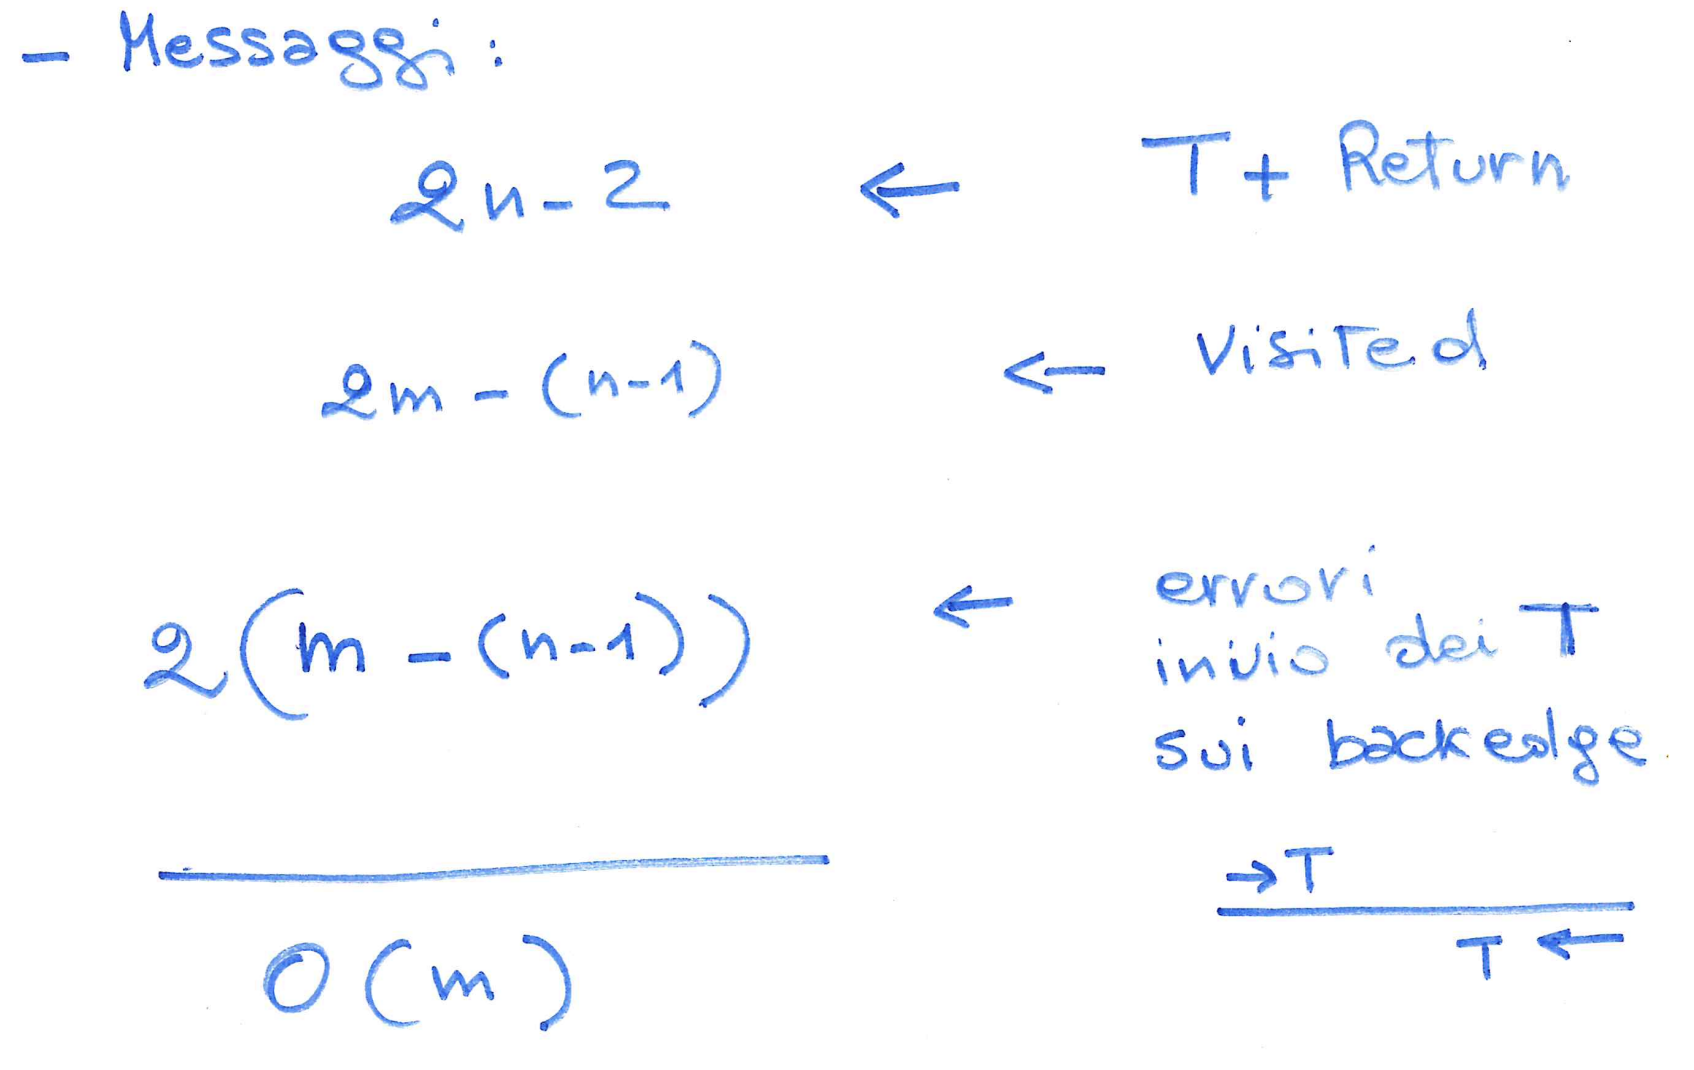
\includegraphics[scale=0.4]{images/traversal.png}
    \caption{Traversal: nuova complessità}
\end{figure}

Abbiamo aumentato il numero di messaggi però abbiamo acccelerato il protocollo.

\paragraph{Nuovo tempo}

Chiamiamo DF* il protocollo modificato con l'idea dei messaggi visited ed è ottimo per M[DF*] e T[DF*]

\subsection{Problemi rivolti all'utente finale}
\subsubsection{Spanning tree}
Costruire un'albero sulla rete dove i nodi sono un'entità di calcolo.

\begin{osservazione}
    I problemi Broadcast(BD), Wake-Up(WP), Traversal (TR) hanno una complessità di messaggi $\Theta(m)$ con 
    $$n - 1 \leq m \leq \frac{n\;(n-1)}{2} = O(n^2)$$
\end{osservazione}
dove a sinistra abbiamo l'albero, a destra il grafo completo

Lo spanning tree è importante perchè \uline{al posto di usare l'intera rete G  del grafo} (che potrebbe anche essere un grafo completo $\frac{n\;(n-1)}{2}$) \uline{usiamo una sotto-rete per minimizzare la complessità di comunicazione}, quale sottorete conviene scegliere? Quella che mi da un numero di archi $n-1$, quindi un albero

 \uline{Data una rete, costruire un albero sulla rete, così da usare l'albero per risolvere gli altri problemi}. Attenzione però ai costi per risolvere i problemi
 \begin{itemize}
     \item Costo di costruzione dell'albero
     \item Costo originale del problema eseguito su di un albero
 \end{itemize}

\paragraph{Il problema dello spanning tree}
Vogliamo costruire una sotto-rete t.c.
\begin{itemize}
    \item Coinvolge tutte le entità
    \item Le entità sono connesse
    \item E' priva di cicli
\end{itemize}

La soluzione con un algoritmo distribuito richiede la conoscenza dell'albero all'interno della rete. \uline{Ogni entità vedrà una piccola parte dell'albero}

\paragraph{Il protocollo Shout}
Shout significa 'urla, chiedi'. Ogni entità chiederà alle altre entità se esse vogliono diventare vicini nell'albero che si sta costruendo.
\begin{itemize}
    \item Ogni entità vede solo i suoi Tree\_N(x)
    \item Tiene traccia del padre
\end{itemize}

La radice dell'albero che si va a costruire è data dall'entità che inizia il protocollo (unico initiator). \uline{Si tiene traccia della radice con una variabile booleana chiamata \textit{root}, un'entità avrà root $=$ True, le altre root $=$ False}.

\begin{itemize}
    \item Iniziatore s(root) spedisce la domanda Q ai suoi vicini e attende le risposte. Chiede sostanzialmente se vogliono diventare i propri figli nell'albero
    \item Ogni entità $x \neq s$ che riceve Q
    \begin{itemize}
        \item la prima volta risponde 'yes', definendo chi è il padre cioè a chi ha inviato la risposta 'yes', ed invia Q ai suoi vicini e si mette in attesa
        \item una volta successiva alla prima risponde 'no'
    \end{itemize}
    \item Inoltre serve memorizzare l'entità padre e le entità che rispondono 'yes'
    \item L'entità termina quando riceve tutte le risposte. Bisognerà tenere traccia di quante risposte riceve, se il numero di messaggi $\text{yes}+\text{no} = Q$ può terminare
\end{itemize}

\uline{Il protocollo Shout è sostanzialmente Flooding + Reply}, perchè si fa una diffusione del messaggio Q nella rete e al messaggio Q bisogna rispondere con un 'yes' oppure un 'no'

\begin{figure}[h]
    \centering
    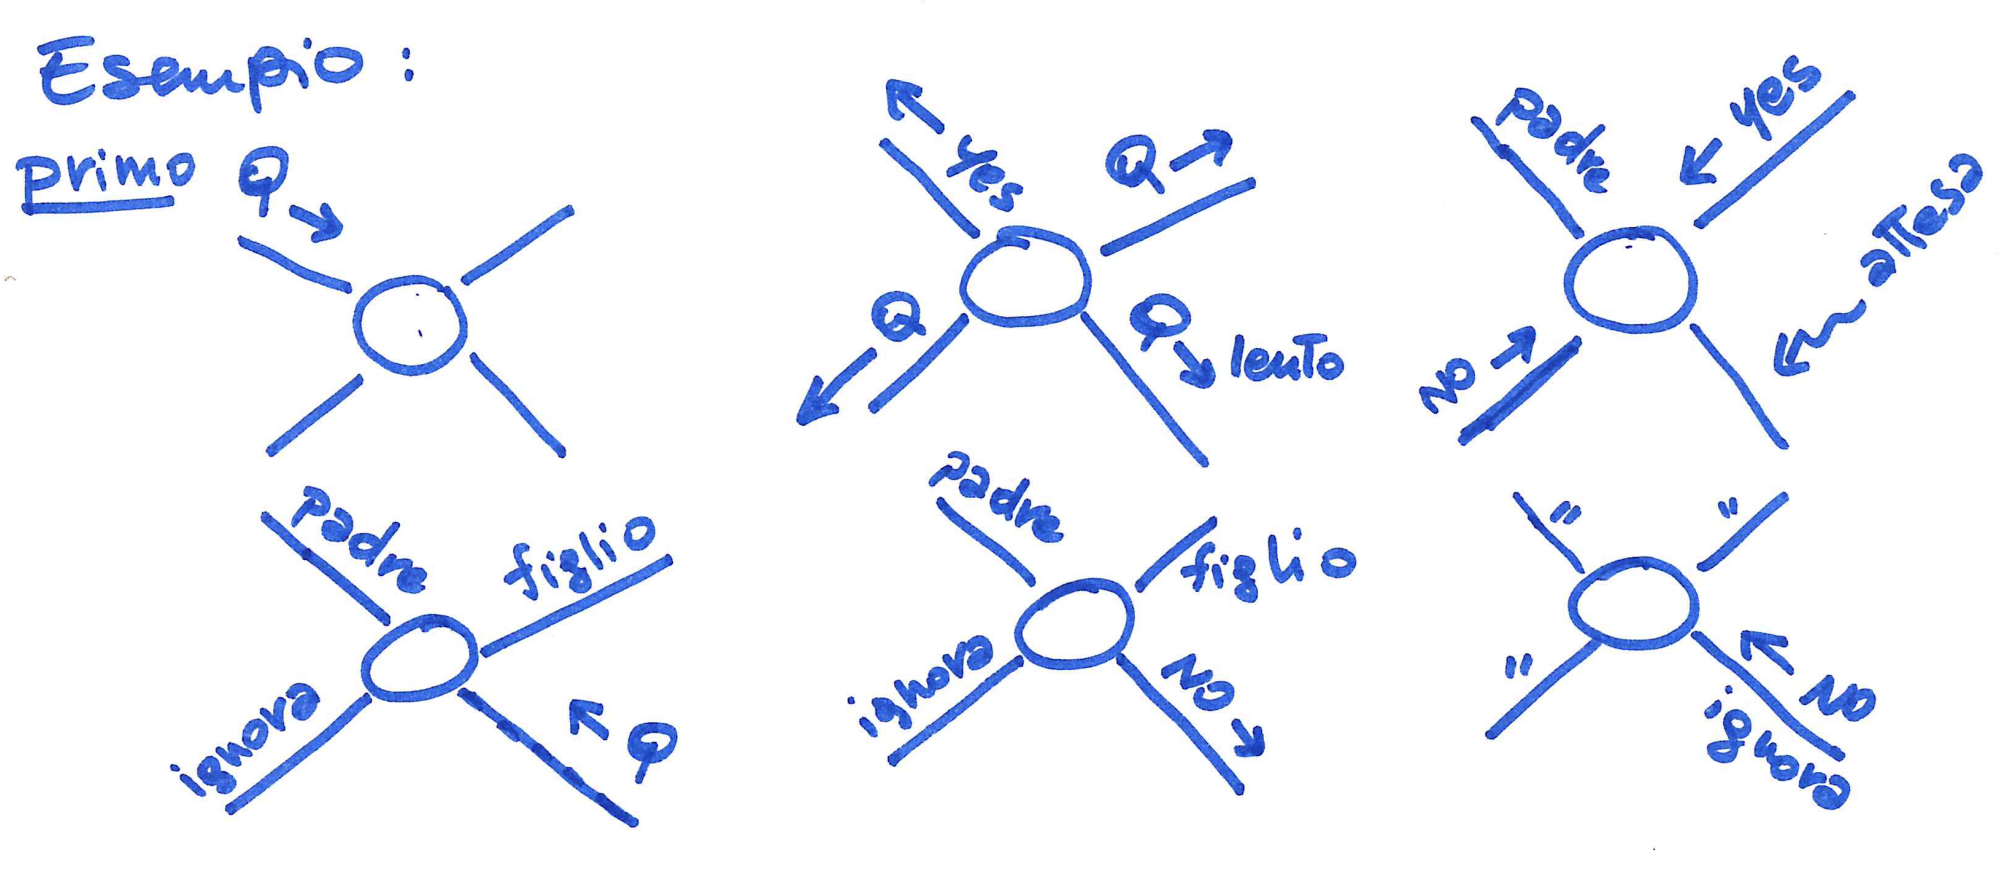
\includegraphics[scale=0.4]{images/protocollo_shout.png}
    \caption{Shout: Flooding + Reply}
    \label{fig:my_label}
\end{figure}

\paragraph{Linee guida per definire il codice}
\begin{itemize}
    \item Mandare i messaggi: Q(question), yes, no
    \item Ogni entità ha la visibilità locale dell'albero. Aggiornare variabili locali: root, parent, Tree\_n(x)\footnote{Vicini di albero: padre, figlio}, counter\footnote{Contatore che conta il numero di risposte ricevute per Q e che gli permette di terminare correttamente}
    \item Aggiornare lo stato, per raggiungere la terminazione
\end{itemize}

\paragraph{Codice}
.\\$Stati = \{\text{iniziatore}, \text{inattivi}, \text{attivi}, \text{finito}\}$\\
$S_{init} = \{\text{iniziatore}, \text{inattivi}\}$\\
$S_{final} = \text{finito}$

\begin{lstlisting}
Iniziatore
    impulso spontaneo
    {
        root = True 
        counter = 0
        tree_N(x) = empty
        send(Q) to N(x);
        become attivo;
    }
    
Inattivo
    ricezione(Q)
    {
        root = false;
        parent = sender;
        counter = 1;
        tree_N(x) = {sender};
        send('yes') sender;
        if counter = |N(x)| then
            become finito;
        else {
            send(Q) to N(x)\sender;
            become attivo;
        }
    }

Attivo
    ricezione(Q)
    { send('no') to sender }
    
    ricezione('yes')
    {
        Tree_N(x) = Tree_N(x).union{sender};
        counter = counter + 1;
        if(counter = |N(x)|) then //ha finito di ricevere le risposte
            become finito;
    }

    ricezione('no')
    {
        counter = counter + 1;
        if(counter = |N(x)|) then
            become finito;
    }
\end{lstlisting}
Solo l'iniziatore ha root True perchè abbiamo una sola radice. L'iniziatore non ha \textit{parent} perchè radice non ha padre.

Quando si riceve un 'no' praticamente il vicino non vuole essere il figlio dell'entità x, quindi non si aggiorna Tree\_N(x)
   
Nello stato finito l'unica azione che si può eseguire è quella nulla, ci si aspetta che quando tutte le entità siano in stato finito l'albero sia già stato costruito

\paragraph{Correttezza}
\begin{itemize}
    \item Terminazione: in assenza di errori riceve un numero di risposte pari ai Q inviati (le entità che seguono il protocollo Shout sono obbligate a rispondere), diventando finito
    \item Tutte le entità sono presenti/coinvolte, grazie al flooding di Q. Tutte le entità ricevono almeno un Q e vengono svegliate
    \item Le entità sono connesse
    \item E' priva di cicli: perchè ogni entità risponde con un solo 'yes' tranne la radice che risponde sempre 'no'. \uline{Per creare un ciclo si deve rispondere 'yes' almeno a due Q}
\end{itemize}

\paragraph{Costi}
Numero di messaggi
$$M[\text{Shout}] = 2M[\text{Flooding}] = 2[2n - (n-1)] = \;\approx 4m$$

Perchè su ogni link viaggia eventualmente un Q in una direzione e un Q in un'altra direzione e poi le risposte 'yes' o 'no' in una direzione e in un'altra direzione, perciò $4$ volte \textit{m}

\paragraph{Tempo}
$$T[\text{Shout}] = T[\text{Flooding}] + 1 \leq d + 1$$

E' essezialmente il tempo di diffusione del Q. Il tempo del Flooding è il diametro

\paragraph{Lower bound}
m per i messaggi, d per il tempo. Quindi abbiamo un protocollo ottimale perchè è $O(m)$ e come tempo $d+1$

\paragraph{Shout migliorato: Shout+}
Possiamo migliorare il protocollo Shout? Posso eliminare dei messaggi? Ci si chiede se questo $4m$ può essere abbassato

I messaggi che eliminiamo sono i messaggi di risposta.\\
'yes' sono necessari e si tengono, 'no' sono superflui e si possono eliminare

Questo perchè quando un'entità riceve un 'no' vuol dire che il rispondente è stato già attivato da un altro nodo e avrà già fatto il Floooding del proprio Q. \uline{L'entità $x$ attiva fa Flooding e può interpretare una risposta Q come un 'no'}

Se la risposta è un 'no' è perchè l'entità ha già ricevuto in precedenza un Q a cui ha risposto 'yes' inviando contestualmente altri Q $\implies$ se ricevo un Q lo interpreto come un 'no'

\paragraph{Nuovo costo di comunicazione Shout+}.\\
$M[\text{Shout+}] = 2m$, due messaggi soli su link


%Election
\subsubsection{Election}

\paragraph{Scopo} \uline{Stabilire un leader tra le entità di calcolo}. Individuare un'entità specifica tra tante entità autonome e omogenee (peer). Tale entità sarà chiamata \textit{LEADER} e le altre \textit{FOLLOWER}

\paragraph{Risultato di impossibilità}
E' impossibile deterministicamente individuare un leader sotto le restrizioni R (BL, CN, TR) se tutte le unità sono nello stesso stato e hanno i registri allo stesso modo

\paragraph{Risultato di possibilità}
Sotto le restrizioni RI, la starting entity\footnote{Sa di essere la starting entity perchè riceve l'impulso esterno} diventa immediatamente leader, \uline{il problema però è risolto dall'esterno e non dal sistema}. Chi stabilisce qual'è l'entità leader? Non lo stabiliscono le entità ma un evento esterno al sistema. Togliere la restrizione UI: unique initiator e ne metteremo un'altra

\paragraph{Nuova restrizione: Initial Distinct Values (ID)}
\uline{Ogni entità ha un proprio nome}. A questo punto le entità non sono più omogenee perchè hanno un elemento che le distingue che è il nome. \uline{Questo nome potrebbe anche essere un numero} 

Notazione: $R \cup \{ID\} = IR$

Sotto restrizioni IR il problema dell'election è risolvibile.

\paragraph{Strategie di soluzione}
\begin{itemize}
    \item [a)] Elect Minimum
    \begin{enumerate}
        \item Trova $id(x)$ minimo e fai $x$ leader
        \item $\forall y \neq x \in E$, y diventa follower
    \end{enumerate}
    \item [b)] Elect Minimum Initiator
    \begin{enumerate}
        \item Trova $id(x)$ minimo tra le sole entità initiator (non c'è la restrizione unique initiator) ed eleggi $x$ leader
        \item $\forall y \neq x \in E$, y diventa follower
    \end{enumerate}
\end{itemize}

\paragraph{Elect Minimum Ring}
Le mie entità sono collegate ad anello. Ogni entità ha due vicini, sinistra e destra. Siccome hanno solo due vicini, quando ricevono il messaggio arriva da uno di loro e l'altro vicino lo chiamiamo \textit{OTHER}

\paragraph{a) Protocollo All The Way}
I messaggi viaggiano intorno all'anello inoltrati dalle entità nella stessa direzione.

Tipo di messaggio sigla, mittente/entità che l'ha generato: ('Election', id(x))

Il messaggio $E$ generato da $y$ fa il giro dell'anello. Questi messaggi che girano sull'anello portano a conoscenza di tutti i nodi i nomi degli altri nodi, in questo modo tutti possono calcolare il minimo. \uline{Ogni entità riesce a collezionare gli id di tutte le entità così da calcolare il minimo}. Tutti riceveranno gli id di tutti

Quando far terminare un'entità? Una volta che $x$ riceve un messaggio con il proprio $id(x)$ sa che il messaggio ha fatto il giro dell'anello, a questo punto non lo inoltra più. Può terminare?
\begin{itemize}
    \item Solo se na ha viste $n$ diversi, se si suppone che le entità siano a conoscenza della dimensione di A ma in questo caso non c'è questa restrizione. Lavoriamo sulle restrizioni IR più il fatto che le entità sono a conoscenza di essere in un anello
    \item \uline{La risposta corretta è no}. Dobbiamo riempire in maniera oppurtuna i messaggi E ('Election', id(x), ... ) per fare terminare correttamente le entità. Aggiungiamo un contatore, il messaggio ha la seguente forma
    \[E = (\text{"Elect."}\;, id(x), \;\text{counter})\]
    \begin{itemize}
        \item Inizialmente l'entità x pone counter = 1
        \item Ogni altra entità $y \neq x$ che inoltra E somma $1$ a counter
        \item Quando E ritorna all'entità $x$ counter è uguale a $n = |A|$, in questo modo riesce a scoprire anche quant'è la dimensione di A
        \item se $x$ ha già ricevuto $n$ diversi id può terminare, altrimenti si mette in attesa
    \end{itemize}
\end{itemize}

\paragraph{Codice}
.\\$Stati = \{\text{Asleep}, \text{awake}, \text{leader}, \text{follower}\}$\\
$S_{init} = \{\text{Asleep}\}$\\
$S_{final} = \{\text{leader}, \text{follower}\}$

\begin{lstlisting}
Asleep
    spontaneously
    {
        INITIALIZE;
        become awake;
    }

    receiving('Elect', value, counter)
    {
        INITIALIZE;
        send('Elect', value, counter + 1) to OTHER
        min = Min{min, value}
        count = count + 1; 
        became awake;
    }

Awake
    receiving('Elect', value, counter)
    {
        if value != id(x) then
        {
            send('Elect', value, counter + 1) to OTHER
            min = Min{min, value}
            count = count + 1; 
            if know = True then CHECK;
            
        } else {
            size = counter;
            know = True;
            CHECK;
        }
    }
\end{lstlisting}

C'è il \textit{counter} nei messaggi che ogni entità deve incrementare e c'è il \textit{count} locale all'interno di ogni entità dove si tiene conto di quanti messaggi diversi ha visto fino a quel momento

\paragraph{Procedure INITIALIZE}
Una procedure in cui si genera il proprio messaggio
\begin{lstlisting}
    count = 0;
    size = 1;
    know = false;
    send('Elect', id(x), size) to right;
    min = id(x);
\end{lstlisting}

\textit{know} diventa True se l'entità riceve il proprio messaggio e viene a scoprire la cardinalità dell'anello

\paragraph{Procedure CHECK} 
E' una procedura che ci permette di controllare se l'entità deve terminare oppure no. Viene invocata quando è conosciuta la dimensione dell'anello.
\begin{lstlisting}
    if count = size then 
        if min = id(x) then
        { become leader; } 
        else { become follower; }
\end{lstlisting}

\paragraph{Complessità}
Numero di messaggi: $M[\text{All the way / IR} \cup \text{Ring}] = n^2$

Troppo costoso, passiamo alla strategia b)

\paragraph{b) Elect Minimum Initiator} 
Solo gli initiator generano E, mentre le altre entità inoltrano il messaggio. Facciamo l'elezione tra le sole entità che startano il protocollo. \uline{Trova l'id minimo tra le sole entità initiator}

\paragraph{Problema di terminazione}
Sebbene ogni entità che ha generato il proprio E facendo girare il messaggio riesce a scoprire il numero $n$ dell'anello, perchè ogni entità che inoltra il messaggio fa counter + 1, \uline{quelle che non hanno generato il proprio messaggio non riescono a scoprire quante entità ci sono nell'anello}. 

La conoscenza è solo delle entità initiator. Sono gli initiator che quando hanno finito e capito chi è il leader possono avvisare le altre entità. In particolare, viene fatto proprio dal leader stesso.

\paragraph{Complessità}
\begin{itemize}
    \item Numero di messaggi\\
    $M[\text{All the way - MinInitiator}] = n * k + n$ dove $k$ è il numero di initiator
    \item Tempo\\
    $M[\text{All the way - MinInitiator}] \leq 3n - 1$ considerando il caso peggiore. 
\end{itemize}

\subsubsection{Shortest Path}
Sempre un problema di comunicazione, cioè due entità che si vogliono inviare messaggi. Ma in questo caso attraverso il cammino migliore\footnote{Il cammino migliore è il cammino più corto in un grafo non pesato, o il cammino di costo minimo in un grafo pesato dove i pesi degli archi rappresentano il costo di attraversamento del messaggio su quell'arco. Questo è preferito perchè appunto abbassa i costi di comunicazione}.

\uline{Devo avere informazioni su tutti i costi della rete}. Richiede l'uso della memoria per registrare informazioni sui costi di $\vec{G}$ per ogni entità $x \in E$ al fine di calcolare i cammini minimi verso ogni altra entità, non solo verso $y$. Risolvendo il problema di comunicazione tra $x,y$ lo facciamo anche $\forall z \neq y$

\paragraph{Restrizioni}
Risolviamo il problema sotto restrizioni IR, quindi classica R + identification number. $\forall x \in E$ abbiamo id(x)

\paragraph{Full Routing Table}
Ogni strategia ha bisogno di questa tabella per risolvere il problema

\paragraph{Protocollo 1: GOSSIPING}
Richiede parecchia memoria.
Prima di costruirsi la Full Routing Table ha bisogno degli id delle entità per poterli scrivere nella colonna \textit{destinazione}

Allora si costruisce \textit{MAP(G)} che altro non è che una matrice di adiacenza\footnote{Un modo di rappresentare il grafo sotto forma tabellare} del grafo. \uline{Alla cella $(i,j)$ abbiamo il peso dell'arco tra i e j}. Abbiamo tutte le entità  sulle righe e sulle colonne e agli incroci i costi tra uno e l'altro. E' una matrice simmetrica rispetto alla diagonale.

In questo protocollo ogni entità vuole costruire questa mappa, che potrebbe essere anche molto grande. Per costruire MAP(G) in un ambiente distribuito è sufficiente che ogni entità $x$ diffonda le proprie informazioni sui vicini ad ogni altra entità $y \in E$ (fare un BROADCAST). Fare un BCAST su tutta la rete è molto costoso, in più dovrebbero farlo tutte le entità. Perciò si potrebbe costruire un albero

\paragraph{MAP-GOSSIP}
\begin{itemize}
    \item Costruzione di un albero T per G
    \item Ogni entità acquisisce dai vicini id ed i costi dei link
    \item Ogni entità diffonde le sue informazioni a tutte le altre entità usando i link di T
\end{itemize}
Una volta costruito MAP(G) ci sono tanti modi per calcolare shortest-path, ad esempio Djkstra

\paragraph{Complessità di MAP-GOSSIP}
\begin{itemize}
    \item Numero di messaggi
    \begin{itemize}
        \item Costruzione spanning tree $O(m + n \log n)$, il migliore
        \item Acquisizione informazioni dei vicini $2m$
        \item Broadcast delle informazioni $2m - 1$
    \end{itemize}
    $$M[\text{Map-Gossip}] \approx 2m * n \approx O(n^2)$$
    Quando $G$ è sparso
    \item Tempo, difficile da calcolare
\end{itemize}

Perchè Map-gossip viene scartato? Perchè non è detto che tutte le entità abbiano abbastanza memoria per mantenere una mappa del grafo, soprattutto se l'ambiente distribuito è molto grande

\paragraph{Protocollo 2: Iterated-Construction}
\uline{Richiede meno memoria} a scapito della congestione dei messaggi spediti. Aumenta anche il tempo

La Full Routing Table viene costruita a più riprese. \uline{Si evita di costruire la MAP(G)} e si va direttamente a costruire la tabella attraverso un processo di iterazioni in cui c'è uno scambio di messaggi tra le entità. \uline{Ogni entità si costruisce la sua Full Routing Table senza utilizzare MAP(G), così evitiamo lo spreco di memoria}. Inizialmente la F.R.T. contiene solo informazioni dei vicini, con costo $\infty$ per i non vicini che verrà sostiuito alle iterazioni successive con un valore più ragionevole

\begin{osservazione}
    Se vogliamo una Routing Table più corta, è possibile che al posto dello \textit{shortest path} ci mettiamo il vicino coinvolto nel cammino. Con questo riusciamo a ridurre la quantità di memoria necessaria
\end{osservazione}

\paragraph{Distance Vector}
Ogni entità si costruisce una F.R.T parziale e ad ogni iterazione questa tabella viene aggiornata, ad ogni iterazione si spedisce ai vicini delle informazioni. Queste informazioni vengono ricevute dalle entità che aggiorna la propria F.R.T. Le informazioni che si spediscono sono il Distance Vector

Sulla base delle informazioni che gli arrivano dai vicini stabilisce se sono stati trovati cammini minimi migliori di quelli che ha nella propria FRT e in tal caso aggiorna la FRT

\paragraph{Notazione} $V_x[z]$ è il costo del cammino minimo da $x$ a $z$

\begin{definizione}
    E' la F.R.T. ristretta alle colonne Destination e Cost e viene indicata con V
\end{definizione}

\paragraph{Numero di iterazioni} $n-1$, si può dimostrare per induzione

\paragraph{Complessità Iterated-Construction}
E' un protocollo con più iterazioni. Il numero di iterazioni è $n-1$
\begin{itemize}
    \item Numero di messaggi
    $$M[\text{ItConstr / IR}] = 2m * n * (n-1)$$
    Su ogni arco abbiamo due spedizioni di Distance Vector che costano $n$, ripetuta per $n-1$ iterazioni
    \item Tempo
    $$M[\text{ItConstr / IR}] = (n-1) * \tau(n)$$
    Ci sono sempre $n-1$ iterazioni dove in ogni iterazioni vengono spediti le V (Distance Vector). $\tau(n)$ è il tempo ideale per trasmettere una V. 
\end{itemize}




%----------------------------------
\end{document}

